% Options for packages loaded elsewhere
\PassOptionsToPackage{unicode}{hyperref}
\PassOptionsToPackage{hyphens}{url}
%
\documentclass[
]{book}
\usepackage{amsmath,amssymb}
\usepackage{iftex}
\ifPDFTeX
  \usepackage[T1]{fontenc}
  \usepackage[utf8]{inputenc}
  \usepackage{textcomp} % provide euro and other symbols
\else % if luatex or xetex
  \usepackage{unicode-math} % this also loads fontspec
  \defaultfontfeatures{Scale=MatchLowercase}
  \defaultfontfeatures[\rmfamily]{Ligatures=TeX,Scale=1}
\fi
\usepackage{lmodern}
\ifPDFTeX\else
  % xetex/luatex font selection
\fi
% Use upquote if available, for straight quotes in verbatim environments
\IfFileExists{upquote.sty}{\usepackage{upquote}}{}
\IfFileExists{microtype.sty}{% use microtype if available
  \usepackage[]{microtype}
  \UseMicrotypeSet[protrusion]{basicmath} % disable protrusion for tt fonts
}{}
\makeatletter
\@ifundefined{KOMAClassName}{% if non-KOMA class
  \IfFileExists{parskip.sty}{%
    \usepackage{parskip}
  }{% else
    \setlength{\parindent}{0pt}
    \setlength{\parskip}{6pt plus 2pt minus 1pt}}
}{% if KOMA class
  \KOMAoptions{parskip=half}}
\makeatother
\usepackage{xcolor}
\usepackage{color}
\usepackage{fancyvrb}
\newcommand{\VerbBar}{|}
\newcommand{\VERB}{\Verb[commandchars=\\\{\}]}
\DefineVerbatimEnvironment{Highlighting}{Verbatim}{commandchars=\\\{\}}
% Add ',fontsize=\small' for more characters per line
\usepackage{framed}
\definecolor{shadecolor}{RGB}{248,248,248}
\newenvironment{Shaded}{\begin{snugshade}}{\end{snugshade}}
\newcommand{\AlertTok}[1]{\textcolor[rgb]{0.94,0.16,0.16}{#1}}
\newcommand{\AnnotationTok}[1]{\textcolor[rgb]{0.56,0.35,0.01}{\textbf{\textit{#1}}}}
\newcommand{\AttributeTok}[1]{\textcolor[rgb]{0.13,0.29,0.53}{#1}}
\newcommand{\BaseNTok}[1]{\textcolor[rgb]{0.00,0.00,0.81}{#1}}
\newcommand{\BuiltInTok}[1]{#1}
\newcommand{\CharTok}[1]{\textcolor[rgb]{0.31,0.60,0.02}{#1}}
\newcommand{\CommentTok}[1]{\textcolor[rgb]{0.56,0.35,0.01}{\textit{#1}}}
\newcommand{\CommentVarTok}[1]{\textcolor[rgb]{0.56,0.35,0.01}{\textbf{\textit{#1}}}}
\newcommand{\ConstantTok}[1]{\textcolor[rgb]{0.56,0.35,0.01}{#1}}
\newcommand{\ControlFlowTok}[1]{\textcolor[rgb]{0.13,0.29,0.53}{\textbf{#1}}}
\newcommand{\DataTypeTok}[1]{\textcolor[rgb]{0.13,0.29,0.53}{#1}}
\newcommand{\DecValTok}[1]{\textcolor[rgb]{0.00,0.00,0.81}{#1}}
\newcommand{\DocumentationTok}[1]{\textcolor[rgb]{0.56,0.35,0.01}{\textbf{\textit{#1}}}}
\newcommand{\ErrorTok}[1]{\textcolor[rgb]{0.64,0.00,0.00}{\textbf{#1}}}
\newcommand{\ExtensionTok}[1]{#1}
\newcommand{\FloatTok}[1]{\textcolor[rgb]{0.00,0.00,0.81}{#1}}
\newcommand{\FunctionTok}[1]{\textcolor[rgb]{0.13,0.29,0.53}{\textbf{#1}}}
\newcommand{\ImportTok}[1]{#1}
\newcommand{\InformationTok}[1]{\textcolor[rgb]{0.56,0.35,0.01}{\textbf{\textit{#1}}}}
\newcommand{\KeywordTok}[1]{\textcolor[rgb]{0.13,0.29,0.53}{\textbf{#1}}}
\newcommand{\NormalTok}[1]{#1}
\newcommand{\OperatorTok}[1]{\textcolor[rgb]{0.81,0.36,0.00}{\textbf{#1}}}
\newcommand{\OtherTok}[1]{\textcolor[rgb]{0.56,0.35,0.01}{#1}}
\newcommand{\PreprocessorTok}[1]{\textcolor[rgb]{0.56,0.35,0.01}{\textit{#1}}}
\newcommand{\RegionMarkerTok}[1]{#1}
\newcommand{\SpecialCharTok}[1]{\textcolor[rgb]{0.81,0.36,0.00}{\textbf{#1}}}
\newcommand{\SpecialStringTok}[1]{\textcolor[rgb]{0.31,0.60,0.02}{#1}}
\newcommand{\StringTok}[1]{\textcolor[rgb]{0.31,0.60,0.02}{#1}}
\newcommand{\VariableTok}[1]{\textcolor[rgb]{0.00,0.00,0.00}{#1}}
\newcommand{\VerbatimStringTok}[1]{\textcolor[rgb]{0.31,0.60,0.02}{#1}}
\newcommand{\WarningTok}[1]{\textcolor[rgb]{0.56,0.35,0.01}{\textbf{\textit{#1}}}}
\usepackage{longtable,booktabs,array}
\usepackage{calc} % for calculating minipage widths
% Correct order of tables after \paragraph or \subparagraph
\usepackage{etoolbox}
\makeatletter
\patchcmd\longtable{\par}{\if@noskipsec\mbox{}\fi\par}{}{}
\makeatother
% Allow footnotes in longtable head/foot
\IfFileExists{footnotehyper.sty}{\usepackage{footnotehyper}}{\usepackage{footnote}}
\makesavenoteenv{longtable}
\usepackage{graphicx}
\makeatletter
\def\maxwidth{\ifdim\Gin@nat@width>\linewidth\linewidth\else\Gin@nat@width\fi}
\def\maxheight{\ifdim\Gin@nat@height>\textheight\textheight\else\Gin@nat@height\fi}
\makeatother
% Scale images if necessary, so that they will not overflow the page
% margins by default, and it is still possible to overwrite the defaults
% using explicit options in \includegraphics[width, height, ...]{}
\setkeys{Gin}{width=\maxwidth,height=\maxheight,keepaspectratio}
% Set default figure placement to htbp
\makeatletter
\def\fps@figure{htbp}
\makeatother
\setlength{\emergencystretch}{3em} % prevent overfull lines
\providecommand{\tightlist}{%
  \setlength{\itemsep}{0pt}\setlength{\parskip}{0pt}}
\setcounter{secnumdepth}{5}
\usepackage{booktabs}
\ifLuaTeX
  \usepackage{selnolig}  % disable illegal ligatures
\fi
\usepackage[]{natbib}
\bibliographystyle{apalike}
\usepackage{bookmark}
\IfFileExists{xurl.sty}{\usepackage{xurl}}{} % add URL line breaks if available
\urlstyle{same}
\hypersetup{
  pdftitle={Ensembles: From Beginner to Expert},
  pdfauthor={Russ Conte},
  hidelinks,
  pdfcreator={LaTeX via pandoc}}

\title{Ensembles: From Beginner to Expert}
\author{Russ Conte}
\date{2024-05-23}

\begin{document}
\maketitle

{
\setcounter{tocdepth}{1}
\tableofcontents
}
\chapter{Welcome!}\label{welcome}

Welcome to Ensembles! This book will guide you through the entire process of building your own ensemble models from beginning to end. It will also give you full access to the Ensembles package that automates the entire process.

I've done my very best to make the book very interesting, fun, and practical. There are lots of examples using real world data with all the steps included.

\begin{figure}
\centering
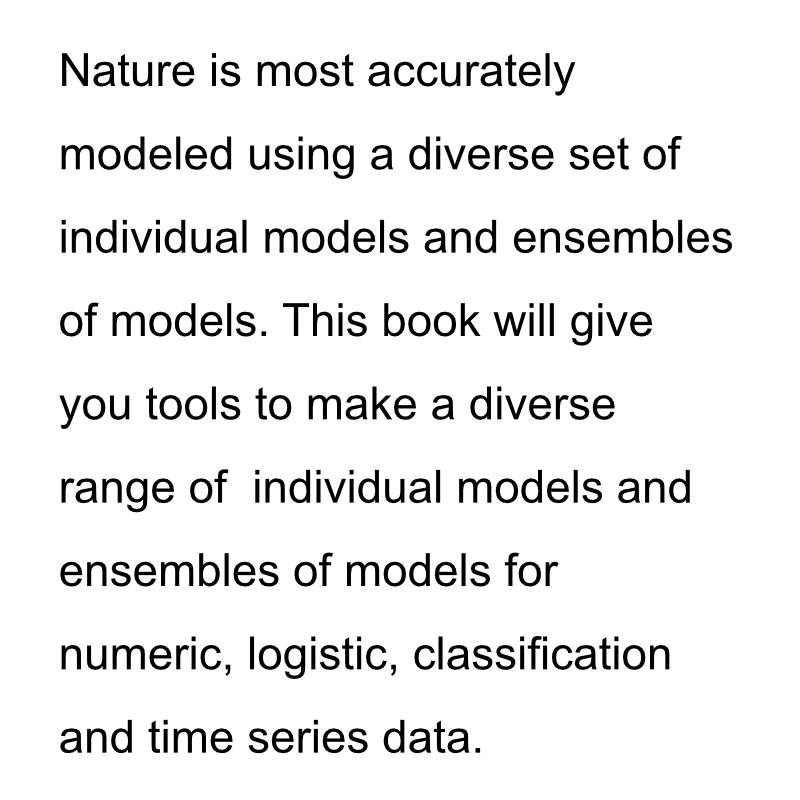
\includegraphics{_book/images/Nature_is_most_accurately_modeled.jpg}
\caption{How nature is most accurately modeled}
\end{figure}

You will be able to do wonderful things as you complete the skills in this book. As the book will show, ensembles are much more accurate than any other method to help us understand and model nature. This will be done with a level of accuracy that has not been achieved previously. And you can do all of it.

The phrase ``wonderful things'' is very intentional. When Howard Carter was doing archaeology, at one point in November, 1922, he was quite sure he found something important. Carter made a small hole to see through. Lord Carnarvon (who was paying for all of this!) asked Howard Carter, ``Can you see anything?. Howard Carter's famous reply,''Yes, wonderful things!{}``. When they opened everything up, they found the intact tomb of Tutankhamun. It contained more than 5,000 items, and enriched our knowledge of ancient Africa beyond any other find.

Here is a tiny taste of one of the more than 5,000 the ``wonderful things'' found by Howard Carter, Lord Carnarvon, and the team of archaeologists.

\begin{figure}
\centering

\includegraphics{_book/images/King_Tut_Mask.jpg}
\caption{King Tut Mask}
\end{figure}

I will do my very best to share many ``wonderful things'' through the entire book as you explore the world of ensembles.

The Ensembles package I've made does the entire analysis process for you automatically. This will put the power of ensembles in your hands, give you the strongest foundation for your work, with the highest degree of accuracy.

All of the examples in the book will come from real data. For example (and there are many more examples in the book):

•~HR Analytics

• Predicting the winning time in the London Marathon

• World's most accurate score to a very difficult classification problem

• Beat the best score in student Kaggle competitions

We will have many more practical examples from a very wide range of fields for you to enjoy.

This book will show you how ensembles improve our understanding of nature, and how you can use ensembles in your work. The results using ensembles are much more accurate than has ever been possible before, and that will be demonstrated over and over again in this book. You will be able to use ensembles to understand the world, and build your own models of data, at a level of accuracy that has not been achieved before.

\begin{figure}
\centering
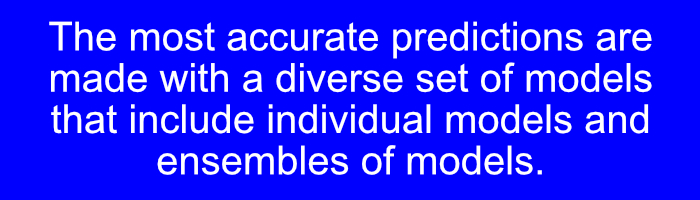
\includegraphics{_book/images/The_most_accurate_predictions.jpg}
\caption{The most accurate predictions}
\end{figure}

\section{Ensembles: The New AI, from beginner to expert}\label{ensembles-the-new-ai-from-beginner-to-expert}

As you will see, Ensembles are the new AI. Science has gone from the calculus of Newton and Leibnetz, to differential equations, to the modern world of creating models, and many points in-between. Ensembles are the most powerful way to put models together to achieve the best possible results. This book will guide you through the process, and show you how you can build ensembles that will pass all testing.

This is the new AI. Welcome to the path, it's extremely fun, and I look forward to sharing it with you!

\section{What you will be able to do by the end of the book}\label{what-you-will-be-able-to-do-by-the-end-of-the-book}

• Make your own customized ensembles of models of numerical, classification, logistic and time series data.

• Use the Ensembles package which does the entire process automatically (but little customization is possible).

• Make your ensemble solutions into packages that can be shared with other users.

• Make your ensemble solutions into totally self-contained solutions that can be shared with anyone.

• Learn how ensembles of models can help to make the wisest possible decision based on the data.

•~Learn how to present the results at different levels, from a regular user to a CEO and board of directors.

• How to present results that are social media friendly.

• Find your own data and create the ensemble solution from beginning to end (called One Of Your Own in the each of the chapter exercises)

• Solve real world examples in this book where ensembles achieve such results as:

• Beat the top score in a student data science competition by over 90\% (numerical ensembles).

• Correctly predict the winning time for the 2024 Men's London Marathon (time series ensembles).

• Produce a 100\% accurate solution to the dry beans classification problem (first in the world with this data set, done using classification ensembles).

• Make recommendations how Lebron James can improve his performance on the basketball court (logistic ensembles).

• Complete a comprehensive Final Project that will put all of your new skills with ensembles together. This result can be shared with employers, advisors, on social media, job interviews, or anywhere else you would like to share your work.

\section{How this book is organized so you learn the material as easily as possible}\label{how-this-book-is-organized-so-you-learn-the-material-as-easily-as-possible}

The book begins with the foundations of making ensembles of models. We will look at:

• Individual numerical models

• Ensembles of numerical models

• Individual classification models

• Ensembles of classification models

• Individual logistic models

• Ensembles of logistic models

• Individual forecasting models

• Ensembles of forecasting models

• Advanced data visualizations

• Multiple ways to communicate your results. This will range from other people in the field, to customers, to the C-Suite (CEO, CTO, board of directors, etc.)

•~We will look at how to treat data science as a business. In particular we will pay close attention to showing return on investment (ROI) in data science, using ensembles of models.

• The book will conclude showing eight examples of a final comprehensive project. There will be two examples each of numerical data, classification data, logistic data and forecasting data. One example of each pair is a regularly formatted paper, the other is professionally formatted. The source files for each of the eight files are available in a github repository.

\section{How you can learn the skills as fast as possible: How the exercises are organized}\label{how-you-can-learn-the-skills-as-fast-as-possible-how-the-exercises-are-organized}

As a young child, I learned that I have much better retention with a system I have always called delayed repetition. This means that I learn best and fastest when I see a worked out example, do several practice examples, and then repeat that after a delay in time. The delay can range from an hour to a few days.

For example, the exercises in the Individual Classification Models chapter will ask you to build models using techniques from the classification models and the prior chapters. The exercises for logistic ensembles will ask you to build models from the content in the logistic models chapter, and each of the previous chapters. It has been my experience that repeating this over and over is the fastest way for me to learn new content, and retain it for the longest period of time.

By the time you get to the Final Comprehensive Project, your skills will be sharp for each of the modeling techniques.

\section{Going from student to teacher: You are required to post on social media and help others understand the results}\label{going-from-student-to-teacher-you-are-required-to-post-on-social-media-and-help-others-understand-the-results}

One of the most important parts of your role in data science is communicating your findings. I will present many examples of summaries and reports for you to adapt and use on your projects. You are also required to post your results on social media. You may use any appropriate choice of social media, but it needs to be publicly available. This has a number of very important benefits to you:

• You will build a body of work that shows your skill level

• The results will demonstrate your ability to communicate in a way that works with a wide variety of people

• You will work to demonstrate very good skills with video and/or audio production

• Use the hashtag \#AIEnsembles when you post on social media

\section{Helping you use the power of pre-trained ensembles and individual models}\label{helping-you-use-the-power-of-pre-trained-ensembles-and-individual-models}

Another important part of the skills you will learn here includes building pre-trained ensembles and models. The book will walk you through the process of building the pre-trained models and ensembles for each of the four types of data (numerical, classification, logicial, and time series).

\section{Helping you master the material: One of your own exercises}\label{helping-you-master-the-material-one-of-your-own-exercises}

One of the differences with the exercises in Ensembles is the inclusion of One of Your Own exercises. Each set of exercises will include one which asks you to find your own data (with many hints given to help you find data), define the problem, make the ensemble, and report the results.

\begin{figure}
\centering
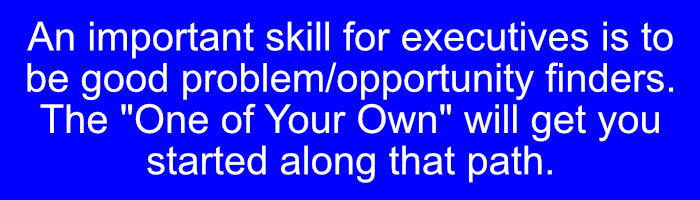
\includegraphics{_book/images/Good_problem_finder.jpg}
\caption{Good problem finder}
\end{figure}

\section{Keeping it real: Actual business data and problems as the source of all the data sets}\label{keeping-it-real-actual-business-data-and-problems-as-the-source-of-all-the-data-sets}

All of the data sets in this book use real data. No exceptions, no synthetic data. The sources of the data are all cited, and the real world implications can be found by a simple search. All of the data is absolutely real.

\section{Helping you check your work---and verifying that your results beat previously published results}\label{helping-you-check-your-workand-verifying-that-your-results-beat-previously-published-results}

Many of the data sets have been solved by previous investigators (such as in competitions), so the results here can be easily compared with published results.

For example, we will look at the Boston Housing data set when we look at numerical data sets. This data set has been used many times in Kaggle competitions, published papers, and Github repositories, among many other sources.

The Ensembles package will automatically solve this data set, and return an RMSE less than 0.20 (there will be slight variation depending on how the parameters are set, as will be explained those chapters). In comparison, the Boston Housing data set was used in this Kaggle student competition: \url{https://www.kaggle.com/competitions/uou-g03784-2022-spring/leaderboard?tab=public}, and the best score was 2.09684. The Ensembles package will beat the best result in that Kaggle student competition by more than 90\%. The Ensembles package only requires one line of code.

\section{Helping you work as a team with fully reproducible ensembles and individual models}\label{helping-you-work-as-a-team-with-fully-reproducible-ensembles-and-individual-models}

A large part of the skills you will learn include how to make results that are reproducible. This will include:

• Multiple random resamplings of the data

• Learning how to test on totally unseen data for both individual and ensemble models

• How to repeat results (for example, 25 times), and report the accuracy of each resampling

For example, you will make ensembles of models, and then use those trained models to make predictions on totally unseen data.

\section{The Final Comprehensive Project will put everything together for you}\label{the-final-comprehensive-project-will-put-everything-together-for-you}

As I was studying data science, one of my professors said that the papers I turned in were ``good enough to show to the CEO or Board of Directors'' of the Fortune 1000 company he worked for. The chapter on the Final Comprehensive Project will share the highest level of skills in the following:

• Truly understanding the business problem

• Being able to convey the very high value that data science brings to the table

• Being able to back up 100\% of your claims with rock solid evidence, facts, and clear reasoning

• How to make a truly professional quality presentation worthy of the C-Suite

\begin{figure}
\centering
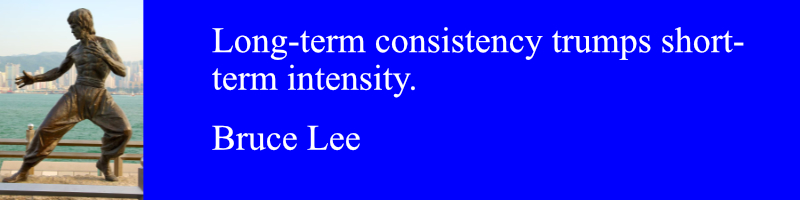
\includegraphics{_book/images/Bruce_Lee.jpg}
\caption{Long term consistency wins the race}
\end{figure}

I've had the incredible pleasure of learning many different skills. A few include being able to play on more than 20 musical instruments, communicate in three languages at a professional level, manage a multi-million dollar division of a Fortune 1000 company, run two non-profit volunteer groups, snowboard a three mile run in Colorado, work as a professional counselor, and much more. The book your reading is only my most recent project. None of these skills were acquired overnight. A huge part of the success is being able to make slow and (usually) steady progress. The next chapter will reveal the big secret to getting results, but for now you are best off if you plan some regular time to work on the contents of the book.

Always remember to test everything, that will save you a ton of problems down the road.

\section{Exercises to help improve your skills}\label{exercises-to-help-improve-your-skills}

Exercise 1: Schedule regular time to work on this book

You will gain much more progress if you work at a steady pace. Take everything in small pieces. It's OK to go slow, as long as you keep going. Schedule regular time to work on this book, and you will get the largest possible reward for your efforts.

Exercise 2: Read each chapter at least twice \textbf{before} you begin working on the material.

Reading each chapter twice before you begin working on it will actually speed up your progress and results. It will actually take less time for you to complete the chapter. You might not believe it right now, but it's totally true.

Exercise 2a: Read a chapter ahead if you are able to do so.

Exercise 3: Read this chapter again

\chapter{Introduction and your first ensembles}\label{introduction-and-your-first-ensembles}

\section{How a Chicago blizzard led to the very unlikely story of the best solutions to supervised data}\label{how-a-chicago-blizzard-led-to-the-very-unlikely-story-of-the-best-solutions-to-supervised-data}

My journey to the most advanced AI in the world started with an actual
blizzard in Chicago. It might seem like Chicago would never get a
blizzard, but we did in 2011, and it was incredibly intense, as this
video shows:

\url{https://www.youtube.com/watch?v=cPiFn52ztd8}

What does the \href{https://en.wikipedia.org/wiki/2011_Groundhog_Day_blizzard}{Chicago 2011
Snomageddon}
have to do with the creation of the most advanced AI? Everything. Here's
the story.

At the time of the 2011 Blizzard I worked a Recruiter for \href{https://en.wikipedia.org/wiki/Kelly_Services}{Kelly
Services}, where I had
worked since 1996. I agreed to work out of the Kelly Services office in
Frankfort, Illinois at this time, though I worked out of nearly every
Kelly Services office at one time or another. The trip to Frankfort
involved a daily commute to the office, but I was able to make the best
use of the time on the road.

My manager at the time let me know several days in advance that there
was a very large amount of snow forecast, and that I might want to be
prepared. The most recent forecasts for large amounts of snow in the
Chicago area all amounted to nothing. They were perfectly normal days in
the Chicago area, so I predicted this storm would also be nothing, based
on the most recent results. This was a great example of a prior
prediction not transferring well to a current situation.

That morning I went to work as normal, and did not even look at the
weather forecast. Around 2:45 pm my manager came out of her office and
said ``Russ, you need to come here and look at the weather radar!''. I
walked into her office, and saw a map of a winter storm that was
incredibly huge. She had the image zoomed out, so it was possible to see
several states. From what I could tell, the massive snow storm was
barreling down on Chicago, and was about 15 minutes away from our
location.

I told the candidate I was interviewing that I was leaving immediately,
and that he is not allowed to stay. He has to get home as fast as
possible for his own safety.

The storm started dropping snow on my trip north back home. The commute
took around 50\% longer than normal due to the rapidly falling snow.

As I later learned, the storm was forecast to start in the Chicago area
around 3:00 pm, finish up between 11:00 am - 1:00 pm two days later, and
leave 17 - 19 inches of snow.

How bad was it? Even City of Chicago snow plows were stopped by the
snow:

\begin{figure}
\centering
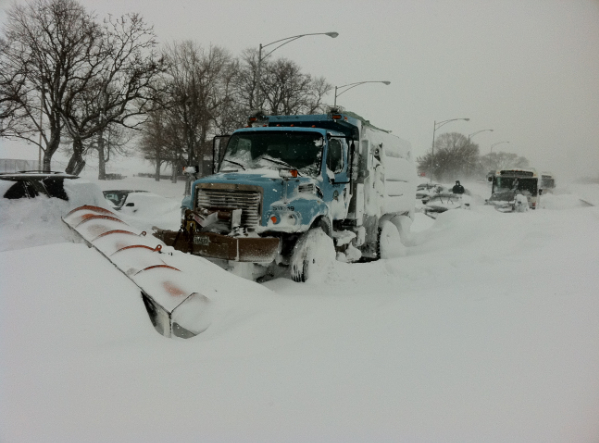
\includegraphics{_book/images/Chicago_Snow_Plow_stuck_on_Lake_Shore_drive_Chicago_Feb_2_2011_storm.jpg}
\caption{\href{https://en.wikipedia.org/wiki/2011_Groundhog_Day_blizzard\#/media/File:Stuck_Salt_Truck_on_Lake_Shore_drive_Chicago_Feb_2_2011_storm.JPG}{Chicago snow
plow}
stuck on Lake Shore Drive in the 2011 snow
storm}
\end{figure}

To see what the forecasts looked like, check out this news report from
the day:

\url{https://www.nbcchicago.com/news/local/blizzard-unleashes-winter-fury/2096753/}

It turns out all three predictions of the blizzard were accurate to a
level that almost seemed uncanny to me: Start time, accumulation, and
end time were all spot on. This is the first time I recall ever seeing a
prediction at this level of accuracy. I had no idea this type of
predictive accuracy was even possible. This level of accuracy in
predicting results totally blew me away. I had never seen anything with
this level of accuracy, and now I wanted to know how it was done.

I searched and searched for how the accuracy was so high for this
forecast.

The power of the method---whatever it was---was obvious to me. I realized
that if it could work for the weather, the solution method could work in
an incredibly broad range of situations. A few of many other areas
include business forecasts, production work, modeling prices, and much,
much more. But that this point I had no idea how the accurate prediction
was done.

Some months later a person wrote to \href{https://en.wikipedia.org/wiki/Tom_Skilling}{Tom
Skilling}, chief
meteorologist for WGN TV in Chicago. Tom posted an answer that opened up
the solution for me. Here is the relevant part of \href{https://www.facebook.com/TomSkilling/posts/531146448370303}{Tom Skilling's
answer} to a
2011 storm how the forecast was so accurate:

\begin{quote}
The Weather Service has developed an interesting ``SNOWFALL ENSEMBLE
FORECAST PROBABILITY SYSTEM'' which draws upon a wide range of snow
accumulation forecasts from a whole set of different computer models.
By ``blending'' these model projections, probability of snowfalls
falling within certain ranges becomes possible. Also, this ``blending''
of multiple forecasts ``smooths'' the sometimes huge model disparities
in the amounts being predicted. The resulting probabilities therefore
represent a ``best case'' forecast.
\end{quote}

So that was the first step. Ensembles were the way they achieved such
extraordinary prediction accuracy.

My next goal was to figure out how ensembles were made. As I looked up
information, it became obvious that ensembles had been used for a while,
such as the winning entry in the Netflix Prize Competition:

\begin{figure}
\centering
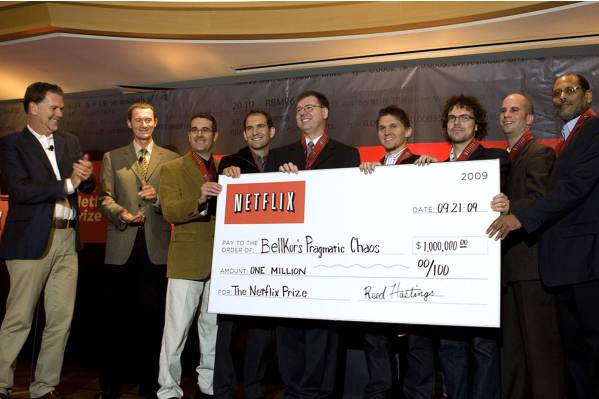
\includegraphics{_book/images/netflix_prize.jpg}
\caption{Netflix Prize Competition}
\end{figure}

The \href{https://en.wikipedia.org/wiki/Netflix_Prize}{Netflix Prize
Competition} was sponsored
by Netflix to create a method to accurately predict user ratings on
films. The minimum winning score needed to beat the Netflix method
(named Cinematch) by at least 10\%. Several years of work went into
solving this problem, and the results even included several published
papers. The winning solution was an ensemble of methods that beat the
Cinematch results by 10.09\%.

So it was now clear to me that ensembles were the path forward. However,
I had no idea how to make ensembles.

I went to graduate school to study data science and predictive
analytics. My degree was completed in 2017, from Northwestern
University. However, I still was not sure how ensembles of models were
built, nor could I find any clear methods to build them (except for
pre-made methods, such as random forests). While it is true there were
packages that could do some of the work, nothing I found did what I was
looking for: How to build ensembles of models in general. Despite
playing with the idea and looking online, I was not able to build the
ensembles I wanted to build.

\section{Saturday, October 15, 2022 at 4:58 pm. The exact birth of the Ensembles system}\label{saturday-october-15-2022-at-458-pm.-the-exact-birth-of-the-ensembles-system}

Everything changed on Saturday, October 15, 2022 at 4:58 pm. I was
playing with various methods to make an ensemble, and got an ensemble
that worked for the very first time. While the results were extremely
modest by any standards, it was clear to me that the foundation was
there to build a general solution that can work in an extremely wide
range of areas. Here is my journal entry:

\begin{figure}
\centering
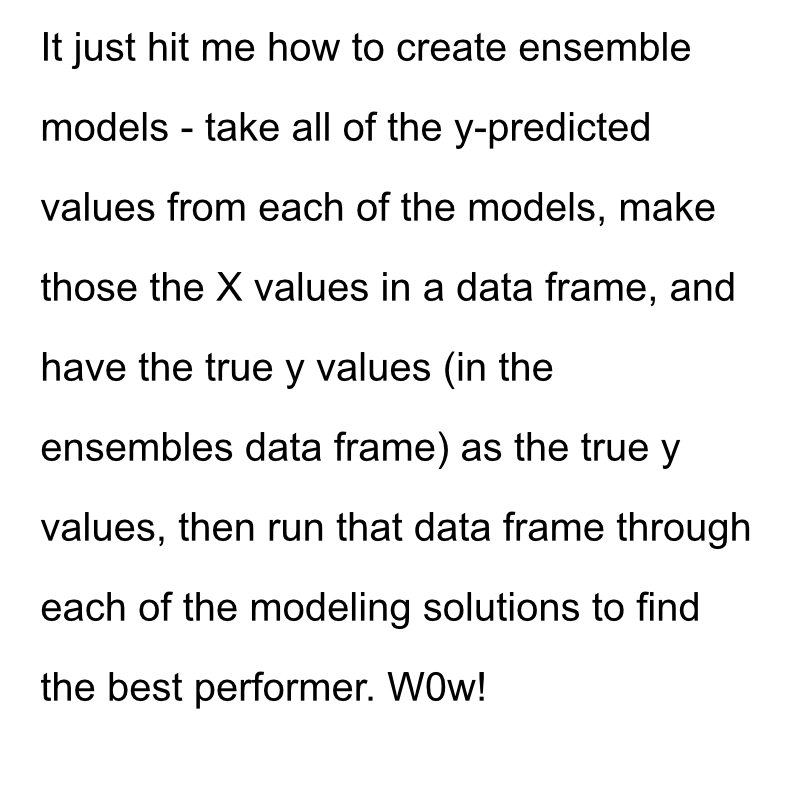
\includegraphics{_book/images/Birth_of_ensembles.jpg}
\caption{Birth of the ensembles method (typo of W0w in the
original)}
\end{figure}

You might be asking yourself how I know the day and time. That is a very
reasonable question. I've been keeping a journal since I was 19 years
old, and have thousands of entries. As soon as I realized how to
correctly build ensembles, I made this entry, which contains the key
elements to make an ensemble, and we will do these steps in just a
moment. Notice that the subject line in the journal matches the text
above.

One of the ways to improve your skills is to keep a journal, and we'll
be looking at that in more depth in this chapter and future chapters.
The journal I use is \href{https://danschimpf.com/}{MacJournal}, though there
are a large number of other options available on the market.

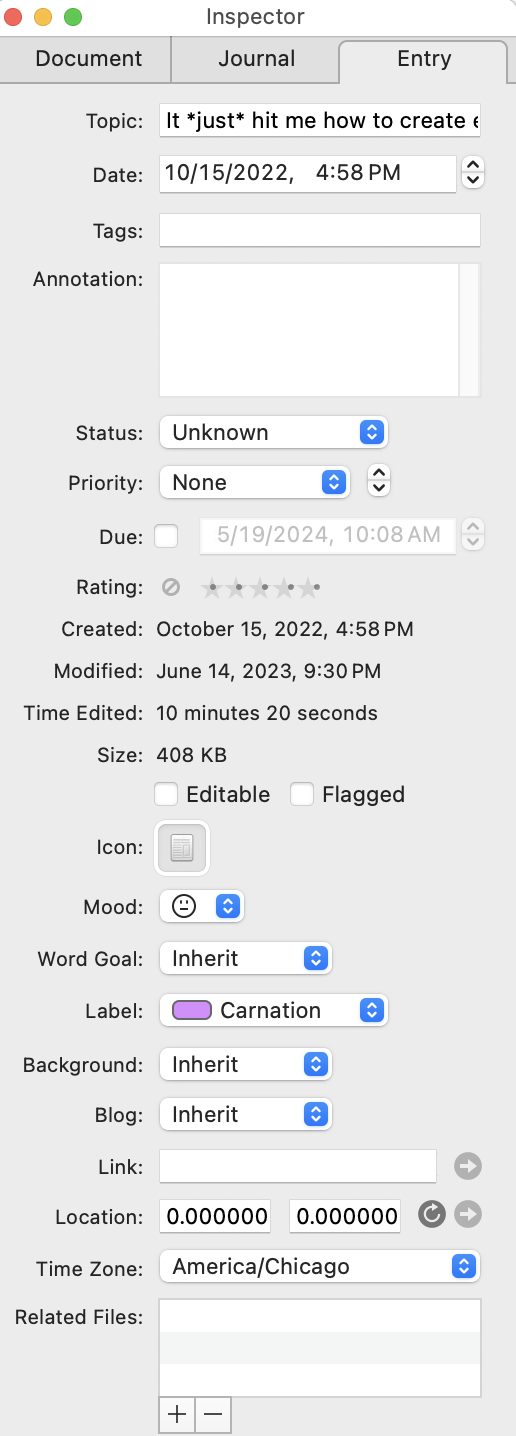
\includegraphics{_book/images/Journal_birth_of_ensembles.png}

Birth of ensembles, Saturday, October 15, 2022 at 4:58 pm

\begin{figure}
\centering

\includegraphics{_book/images/Keep_a_journal.jpg}
\caption{Keep a journal}
\end{figure}

\section{Here is what an ensemble of models looks like at the most basic level, using the Boston Housing data set as an example:}\label{here-is-what-an-ensemble-of-models-looks-like-at-the-most-basic-level-using-the-boston-housing-data-set-as-an-example}

\subsection{Head of Boston Housing data set}\label{head-of-boston-housing-data-set}

\begin{figure}
\centering
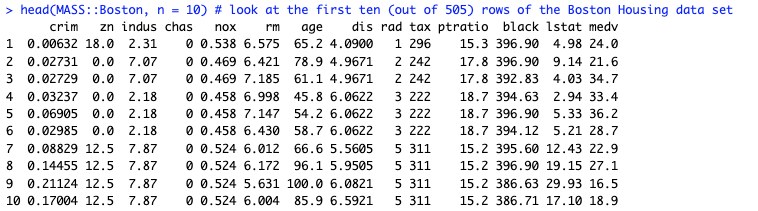
\includegraphics{_book/images/Boston_Housing_data_head.png}
\caption{Head of Boston Housing data
set}
\end{figure}

We will start our first ensemble with a data set that only has numerical
values. Our first example will use the Boston Housing data set, from the
MASS package. While the Boston Housing data set is controversial (and we
will discuss some of the controversies in our example making
professional quality reports for the C-Suite), for now it works as a
very well known data set to begin our journey into ensembles.

Overview of the most basic steps to make an ensemble:

We will be using the Boston Housing data set, so let's have a look at
some Boston images:

\begin{figure}
\centering
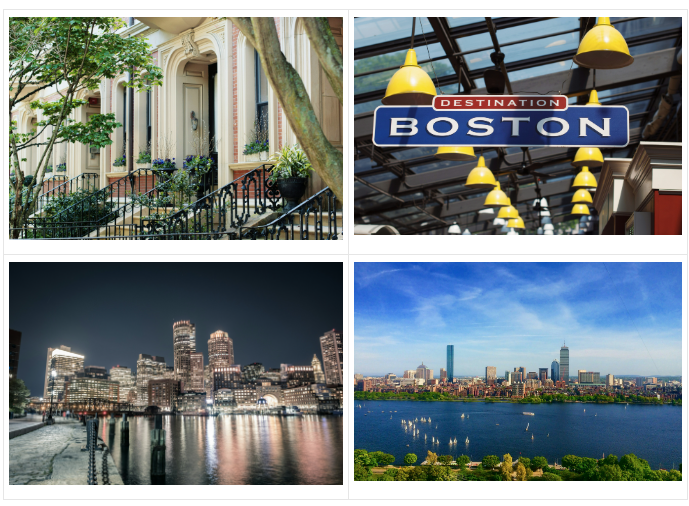
\includegraphics{_book/images/Boston.png}
\caption{Boston}
\end{figure}

\section{The steps to build your first ensemble from scratch}\label{the-steps-to-build-your-first-ensemble-from-scratch}

\begin{itemize}
\item
  Load the packages we will need (MASS, tree)
\item
  Load the Boston Housing data set, and split it into train (60\%) and
  test (40\%) sections.
\item
  Create a linear model by fitting the linear model on the training
  data, and make predictions on the Boston Housing test data. Measure
  the accuracy of the predictions against the actual values.
\item
  Create a model using trees by fitting the tree model on the training
  data, and making predictions on the Boston Housing test data.
  Measure the accuracy of the predictions against the actual values.
\item
  Make a new data frame. This will be our ensemble of model
  predictions. One column will be the linear predictions, and one will
  be the tree predictions.
\item
  Make a new column for the true values---these are the true values in
  the Boston Housing test data set
\item
  Once we have the new ensemble data set, it's simply another data
  set. No different in many ways from any other data set (except how
  it was made).
\item
  Break the ensemble data set into train (60\%) and test (40\%)
  sections.
\item
  Fit a linear model to the ensemble training data. Make predictions
  using the testing data, and measure the accuracy of the predictions
  against the test data.
\item
  Summarize the results.
\end{itemize}

\textbf{I suggest reading the over of the most basic steps to make an ensemble
a couple of times, to make sure you are very familiar with the steps.}

\section{Building the first actual ensemble}\label{building-the-first-actual-ensemble}

Load the packages we will need (MASS, tree):

\begin{Shaded}
\begin{Highlighting}[]
\FunctionTok{library}\NormalTok{(MASS) }\CommentTok{\# for the Boston Housing data set}
\FunctionTok{library}\NormalTok{(tree) }\CommentTok{\# To make models using trees}
\FunctionTok{library}\NormalTok{(Metrics) }\CommentTok{\# To calculate error rate (root mean squared error)}
\FunctionTok{library}\NormalTok{(tidyverse)}
\CommentTok{\#\textgreater{} {-}{-} Attaching core tidyverse packages {-}{-}{-}{-} tidyverse 2.0.0 {-}{-}}
\CommentTok{\#\textgreater{} v dplyr     1.1.4     v readr     2.1.5}
\CommentTok{\#\textgreater{} v forcats   1.0.0     v stringr   1.5.1}
\CommentTok{\#\textgreater{} v ggplot2   3.5.1     v tibble    3.2.1}
\CommentTok{\#\textgreater{} v lubridate 1.9.3     v tidyr     1.3.1}
\CommentTok{\#\textgreater{} v purrr     1.0.2     }
\CommentTok{\#\textgreater{} {-}{-} Conflicts {-}{-}{-}{-}{-}{-}{-}{-}{-}{-}{-}{-}{-}{-}{-}{-}{-}{-}{-}{-}{-}{-} tidyverse\_conflicts() {-}{-}}
\CommentTok{\#\textgreater{} x dplyr::filter() masks stats::filter()}
\CommentTok{\#\textgreater{} x dplyr::lag()    masks stats::lag()}
\CommentTok{\#\textgreater{} x dplyr::select() masks MASS::select()}
\CommentTok{\#\textgreater{} i Use the conflicted package (\textless{}http://conflicted.r{-}lib.org/\textgreater{}) to force all conflicts to become errors}
\end{Highlighting}
\end{Shaded}

Load the Boston Housing data set, and split it into train (60\%) and test
(40\%) sections.

\begin{Shaded}
\begin{Highlighting}[]
\NormalTok{df }\OtherTok{\textless{}{-}}\NormalTok{ MASS}\SpecialCharTok{::}\NormalTok{Boston}
\NormalTok{train }\OtherTok{\textless{}{-}}\NormalTok{ df[}\DecValTok{1}\SpecialCharTok{:}\DecValTok{400}\NormalTok{, ]}
\NormalTok{test }\OtherTok{\textless{}{-}}\NormalTok{ df[}\DecValTok{401}\SpecialCharTok{:}\DecValTok{505}\NormalTok{, ]}

\CommentTok{\# Let\textquotesingle{}s have a quick look at the train and test sets}
\FunctionTok{head}\NormalTok{(train)}
\CommentTok{\#\textgreater{}      crim zn indus chas   nox    rm  age    dis rad tax}
\CommentTok{\#\textgreater{} 1 0.00632 18  2.31    0 0.538 6.575 65.2 4.0900   1 296}
\CommentTok{\#\textgreater{} 2 0.02731  0  7.07    0 0.469 6.421 78.9 4.9671   2 242}
\CommentTok{\#\textgreater{} 3 0.02729  0  7.07    0 0.469 7.185 61.1 4.9671   2 242}
\CommentTok{\#\textgreater{} 4 0.03237  0  2.18    0 0.458 6.998 45.8 6.0622   3 222}
\CommentTok{\#\textgreater{} 5 0.06905  0  2.18    0 0.458 7.147 54.2 6.0622   3 222}
\CommentTok{\#\textgreater{} 6 0.02985  0  2.18    0 0.458 6.430 58.7 6.0622   3 222}
\CommentTok{\#\textgreater{}   ptratio  black lstat medv}
\CommentTok{\#\textgreater{} 1    15.3 396.90  4.98 24.0}
\CommentTok{\#\textgreater{} 2    17.8 396.90  9.14 21.6}
\CommentTok{\#\textgreater{} 3    17.8 392.83  4.03 34.7}
\CommentTok{\#\textgreater{} 4    18.7 394.63  2.94 33.4}
\CommentTok{\#\textgreater{} 5    18.7 396.90  5.33 36.2}
\CommentTok{\#\textgreater{} 6    18.7 394.12  5.21 28.7}
\end{Highlighting}
\end{Shaded}

\begin{Shaded}
\begin{Highlighting}[]
\FunctionTok{head}\NormalTok{(test)}
\CommentTok{\#\textgreater{}         crim zn indus chas   nox    rm   age    dis rad tax}
\CommentTok{\#\textgreater{} 401 25.04610  0  18.1    0 0.693 5.987 100.0 1.5888  24 666}
\CommentTok{\#\textgreater{} 402 14.23620  0  18.1    0 0.693 6.343 100.0 1.5741  24 666}
\CommentTok{\#\textgreater{} 403  9.59571  0  18.1    0 0.693 6.404 100.0 1.6390  24 666}
\CommentTok{\#\textgreater{} 404 24.80170  0  18.1    0 0.693 5.349  96.0 1.7028  24 666}
\CommentTok{\#\textgreater{} 405 41.52920  0  18.1    0 0.693 5.531  85.4 1.6074  24 666}
\CommentTok{\#\textgreater{} 406 67.92080  0  18.1    0 0.693 5.683 100.0 1.4254  24 666}
\CommentTok{\#\textgreater{}     ptratio  black lstat medv}
\CommentTok{\#\textgreater{} 401    20.2 396.90 26.77  5.6}
\CommentTok{\#\textgreater{} 402    20.2 396.90 20.32  7.2}
\CommentTok{\#\textgreater{} 403    20.2 376.11 20.31 12.1}
\CommentTok{\#\textgreater{} 404    20.2 396.90 19.77  8.3}
\CommentTok{\#\textgreater{} 405    20.2 329.46 27.38  8.5}
\CommentTok{\#\textgreater{} 406    20.2 384.97 22.98  5.0}
\end{Highlighting}
\end{Shaded}

Create a linear model by fitting the linear model on the training data,
and make predictions on the Boston Housing test data. Measure the
accuracy of the predictions against the actual values.

\begin{Shaded}
\begin{Highlighting}[]
\NormalTok{Boston\_lm }\OtherTok{\textless{}{-}} \FunctionTok{lm}\NormalTok{(medv }\SpecialCharTok{\textasciitilde{}}\NormalTok{ ., }\AttributeTok{data =}\NormalTok{ train) }\CommentTok{\# Fit the model to the training data}
\NormalTok{Boston\_lm\_predictions }\OtherTok{\textless{}{-}} \FunctionTok{predict}\NormalTok{(}\AttributeTok{object =}\NormalTok{ Boston\_lm, }\AttributeTok{newdata =}\NormalTok{ test)}

\CommentTok{\# Let\textquotesingle{}s have a quick look at the model predictions}
\FunctionTok{head}\NormalTok{(Boston\_lm\_predictions)}
\CommentTok{\#\textgreater{}       401       402       403       404       405       406 }
\CommentTok{\#\textgreater{} 12.618507 19.785728 20.919370 13.014507  6.946392  5.123039}
\end{Highlighting}
\end{Shaded}

Calculate the error for the model

\begin{Shaded}
\begin{Highlighting}[]
\NormalTok{Boston\_linear\_RMSE }\OtherTok{\textless{}{-}}\NormalTok{ Metrics}\SpecialCharTok{::}\FunctionTok{rmse}\NormalTok{(}\AttributeTok{actual =}\NormalTok{ test}\SpecialCharTok{$}\NormalTok{medv, }\AttributeTok{predicted =}\NormalTok{ Boston\_lm\_predictions)}
\NormalTok{Boston\_linear\_RMSE}
\CommentTok{\#\textgreater{} [1] 6.108005}
\end{Highlighting}
\end{Shaded}

The error rate for the linear model is 6.108005. Let's do the same using
the tree method.

Create a model using trees by fitting the tree model on the training
data, and making predictions on the Boston Housing test data. Measure
the accuracy of the predictions against the actual values.

\begin{Shaded}
\begin{Highlighting}[]
\NormalTok{Boston\_tree }\OtherTok{\textless{}{-}} \FunctionTok{tree}\NormalTok{(medv }\SpecialCharTok{\textasciitilde{}}\NormalTok{ ., }\AttributeTok{data =}\NormalTok{ train) }\CommentTok{\# Fit the model to the training data}
\NormalTok{Boston\_tree\_predictions }\OtherTok{\textless{}{-}} \FunctionTok{predict}\NormalTok{(}\AttributeTok{object =}\NormalTok{ Boston\_tree, }\AttributeTok{newdata =}\NormalTok{ test)}

\CommentTok{\# Let\textquotesingle{}s have a quick look at the predictions:}
\FunctionTok{head}\NormalTok{(Boston\_tree\_predictions)}
\CommentTok{\#\textgreater{}      401      402      403      404      405      406 }
\CommentTok{\#\textgreater{} 13.30769 13.30769 13.30769 13.30769 13.30769 13.30769}
\end{Highlighting}
\end{Shaded}

Calculate the error rate for the tree model:

\begin{Shaded}
\begin{Highlighting}[]
\NormalTok{Boston\_tree\_RMSE }\OtherTok{\textless{}{-}}\NormalTok{ Metrics}\SpecialCharTok{::}\FunctionTok{rmse}\NormalTok{(}\AttributeTok{actual =}\NormalTok{ test}\SpecialCharTok{$}\NormalTok{medv, }\AttributeTok{predicted =}\NormalTok{ Boston\_tree\_predictions)}
\NormalTok{Boston\_tree\_RMSE}
\CommentTok{\#\textgreater{} [1] 5.478017}
\end{Highlighting}
\end{Shaded}

The error rate for the tree model is lower (which is better). The error
rate for the tree model is 5.478017.

\section{We're ready to make our first ensemble!!}\label{were-ready-to-make-our-first-ensemble}

Make a new data frame. This will be our ensemble of model predictions,
and one column for the true values. One column will be the linear
predictions, and one will be the tree predictions. We'll make a third
column, the true values.

Make a new column for the true values---these are the true values in the
Boston Housing test data set

\begin{Shaded}
\begin{Highlighting}[]
\NormalTok{ensemble }\OtherTok{\textless{}{-}} \FunctionTok{data.frame}\NormalTok{(}
  \StringTok{\textquotesingle{}linear\textquotesingle{}} \OtherTok{=}\NormalTok{ Boston\_lm\_predictions,}
  \StringTok{\textquotesingle{}tree\textquotesingle{}} \OtherTok{=}\NormalTok{ Boston\_tree\_predictions,}
  \StringTok{\textquotesingle{}y\textquotesingle{}} \OtherTok{=}\NormalTok{ test}\SpecialCharTok{$}\NormalTok{medv}
\NormalTok{)}

\CommentTok{\# Let\textquotesingle{}s have a look at the ensemble:}
\FunctionTok{head}\NormalTok{(ensemble)}
\CommentTok{\#\textgreater{}        linear     tree    y}
\CommentTok{\#\textgreater{} 401 12.618507 13.30769  5.6}
\CommentTok{\#\textgreater{} 402 19.785728 13.30769  7.2}
\CommentTok{\#\textgreater{} 403 20.919370 13.30769 12.1}
\CommentTok{\#\textgreater{} 404 13.014507 13.30769  8.3}
\CommentTok{\#\textgreater{} 405  6.946392 13.30769  8.5}
\CommentTok{\#\textgreater{} 406  5.123039 13.30769  5.0}
\end{Highlighting}
\end{Shaded}

\begin{Shaded}
\begin{Highlighting}[]
\FunctionTok{dim}\NormalTok{(ensemble)}
\CommentTok{\#\textgreater{} [1] 105   3}
\end{Highlighting}
\end{Shaded}

Once we have the new ensemble data set, it's simply another data set. No
different in many ways from any other data set (except how it was made).

Break the ensemble data set into train (60\%) and test (40\%) sections.
There is nothing special about the 60/40 split here, you may use any
numbers you wish.

\begin{Shaded}
\begin{Highlighting}[]
\NormalTok{ensemble\_train }\OtherTok{\textless{}{-}}\NormalTok{ ensemble[}\DecValTok{1}\SpecialCharTok{:}\DecValTok{60}\NormalTok{, ]}
\NormalTok{ensemble\_test }\OtherTok{\textless{}{-}}\NormalTok{ ensemble[}\DecValTok{61}\SpecialCharTok{:}\DecValTok{105}\NormalTok{, ]}

\FunctionTok{head}\NormalTok{(ensemble\_train)}
\CommentTok{\#\textgreater{}        linear     tree    y}
\CommentTok{\#\textgreater{} 401 12.618507 13.30769  5.6}
\CommentTok{\#\textgreater{} 402 19.785728 13.30769  7.2}
\CommentTok{\#\textgreater{} 403 20.919370 13.30769 12.1}
\CommentTok{\#\textgreater{} 404 13.014507 13.30769  8.3}
\CommentTok{\#\textgreater{} 405  6.946392 13.30769  8.5}
\CommentTok{\#\textgreater{} 406  5.123039 13.30769  5.0}
\end{Highlighting}
\end{Shaded}

\begin{Shaded}
\begin{Highlighting}[]
\FunctionTok{head}\NormalTok{(ensemble\_test)}
\CommentTok{\#\textgreater{}       linear     tree    y}
\CommentTok{\#\textgreater{} 461 23.88984 13.30769 16.4}
\CommentTok{\#\textgreater{} 462 23.29129 13.30769 17.7}
\CommentTok{\#\textgreater{} 463 22.54055 21.84327 19.5}
\CommentTok{\#\textgreater{} 464 25.50940 21.84327 20.2}
\CommentTok{\#\textgreater{} 465 22.71231 21.84327 21.4}
\CommentTok{\#\textgreater{} 466 20.83810 21.84327 19.9}
\end{Highlighting}
\end{Shaded}

Fit a linear model to the ensemble training data. Make predictions using
the testing data, and measure the accuracy of the predictions against
the test data. Notice how similar this is to our linear and tree models.

\begin{Shaded}
\begin{Highlighting}[]
\CommentTok{\# Fit the model to the training data}
\NormalTok{ensemble\_lm }\OtherTok{\textless{}{-}} \FunctionTok{lm}\NormalTok{(y }\SpecialCharTok{\textasciitilde{}}\NormalTok{ ., }\AttributeTok{data =}\NormalTok{ ensemble\_train)}

\CommentTok{\# Make predictions using the model on the test data}
\NormalTok{ensemble\_lm\_predictions }\OtherTok{\textless{}{-}} \FunctionTok{predict}\NormalTok{(}\AttributeTok{object =}\NormalTok{ ensemble\_lm, }\AttributeTok{newdata =}\NormalTok{ ensemble\_test)}

\CommentTok{\# Calculate error rate for the ensemble predictions}
\NormalTok{ensemble\_lm\_rmse }\OtherTok{\textless{}{-}}\NormalTok{ Metrics}\SpecialCharTok{::}\FunctionTok{rmse}\NormalTok{(}\AttributeTok{actual =}\NormalTok{ ensemble\_test}\SpecialCharTok{$}\NormalTok{y, }\AttributeTok{predicted =}\NormalTok{ ensemble\_lm\_predictions)}

\CommentTok{\# Report the error rate for the ensemble}
\NormalTok{ensemble\_lm\_rmse}
\CommentTok{\#\textgreater{} [1] 4.826962}
\end{Highlighting}
\end{Shaded}

Summarize the results.

\begin{Shaded}
\begin{Highlighting}[]
\NormalTok{results }\OtherTok{\textless{}{-}} \FunctionTok{data.frame}\NormalTok{(}
  \StringTok{\textquotesingle{}Model\textquotesingle{}} \OtherTok{=} \FunctionTok{c}\NormalTok{(}\StringTok{\textquotesingle{}Linear\textquotesingle{}}\NormalTok{, }\StringTok{\textquotesingle{}Tree\textquotesingle{}}\NormalTok{, }\StringTok{\textquotesingle{}Ensemble\textquotesingle{}}\NormalTok{),}
  \StringTok{\textquotesingle{}Error\textquotesingle{}} \OtherTok{=} \FunctionTok{c}\NormalTok{(Boston\_linear\_RMSE, Boston\_tree\_RMSE, ensemble\_lm\_rmse)}
\NormalTok{)}

\NormalTok{results}
\CommentTok{\#\textgreater{}      Model    Error}
\CommentTok{\#\textgreater{} 1   Linear 6.108005}
\CommentTok{\#\textgreater{} 2     Tree 5.478017}
\CommentTok{\#\textgreater{} 3 Ensemble 4.826962}
\end{Highlighting}
\end{Shaded}

Clearly the ensemble had the lowest error rate of the three models. The
ensemble is easily the best of the three models because it has the
lowest error rate of all the models.

\subsection{Try it yourself: Make an ensemble where the ensemble is made using trees instead of linear models.}\label{try-it-yourself-make-an-ensemble-where-the-ensemble-is-made-using-trees-instead-of-linear-models.}

\begin{Shaded}
\begin{Highlighting}[]
\CommentTok{\# Fit the model to the training data}
\NormalTok{ensemble\_tree }\OtherTok{\textless{}{-}} \FunctionTok{tree}\NormalTok{(y }\SpecialCharTok{\textasciitilde{}}\NormalTok{ ., }\AttributeTok{data =}\NormalTok{ ensemble\_train)}

\CommentTok{\# Make predictions using the model on the test data}
\NormalTok{ensemble\_tree\_predict }\OtherTok{\textless{}{-}} \FunctionTok{predict}\NormalTok{(}\AttributeTok{object =}\NormalTok{ ensemble\_tree, }\AttributeTok{newdata =}\NormalTok{ ensemble\_test)}

\CommentTok{\# Let\textquotesingle{}s look at the predictions}
\FunctionTok{head}\NormalTok{(ensemble\_tree\_predict)}
\CommentTok{\#\textgreater{}      461      462      463      464      465      466 }
\CommentTok{\#\textgreater{} 14.80000 14.80000 18.94286 18.94286 18.94286 18.94286}
\end{Highlighting}
\end{Shaded}

\begin{Shaded}
\begin{Highlighting}[]

\CommentTok{\# Calculate the error rate}
\NormalTok{ensemble\_tree\_rmse }\OtherTok{\textless{}{-}}\NormalTok{ Metrics}\SpecialCharTok{::}\FunctionTok{rmse}\NormalTok{(}\AttributeTok{actual =}\NormalTok{ ensemble\_test}\SpecialCharTok{$}\NormalTok{y, }\AttributeTok{predicted =}\NormalTok{ ensemble\_tree\_predict)}

\NormalTok{ensemble\_tree\_rmse}
\CommentTok{\#\textgreater{} [1] 5.322011}
\end{Highlighting}
\end{Shaded}

How does this compare to our three other results? Let's update the
results table

\begin{Shaded}
\begin{Highlighting}[]
\NormalTok{results }\OtherTok{\textless{}{-}} \FunctionTok{data.frame}\NormalTok{(}
  \StringTok{\textquotesingle{}Model\textquotesingle{}} \OtherTok{=} \FunctionTok{c}\NormalTok{(}\StringTok{\textquotesingle{}Linear\textquotesingle{}}\NormalTok{, }\StringTok{\textquotesingle{}Tree\textquotesingle{}}\NormalTok{, }\StringTok{\textquotesingle{}Ensemble\_Linear\textquotesingle{}}\NormalTok{, }\StringTok{\textquotesingle{}Ensemble\_Tree\textquotesingle{}}\NormalTok{),}
  \StringTok{\textquotesingle{}Error\textquotesingle{}} \OtherTok{=} \FunctionTok{c}\NormalTok{(Boston\_linear\_RMSE, Boston\_tree\_RMSE, ensemble\_lm\_rmse, ensemble\_tree\_rmse)}
\NormalTok{)}

\NormalTok{results }\OtherTok{\textless{}{-}}\NormalTok{ results }\SpecialCharTok{\%\textgreater{}\%} \FunctionTok{arrange}\NormalTok{(Error)}

\NormalTok{results}
\CommentTok{\#\textgreater{}             Model    Error}
\CommentTok{\#\textgreater{} 1 Ensemble\_Linear 4.826962}
\CommentTok{\#\textgreater{} 2   Ensemble\_Tree 5.322011}
\CommentTok{\#\textgreater{} 3            Tree 5.478017}
\CommentTok{\#\textgreater{} 4          Linear 6.108005}
\end{Highlighting}
\end{Shaded}

\subsection{Both of the ensemble models beat both of the individual models in this example}\label{both-of-the-ensemble-models-beat-both-of-the-individual-models-in-this-example}

\section{Principle: What is one improvement that can be made? Use a diverse set of models and ensembles to get the best possible result}\label{principle-what-is-one-improvement-that-can-be-made-use-a-diverse-set-of-models-and-ensembles-to-get-the-best-possible-result}

As we shall see when we go through and learn how to build ensembles, the
numerical method we will use will build 27 individual models and 13
ensembles for a total of 40 results. When the goal is to get the best
possible results, a diverse set of models and ensembles, such as the 40
results for numerical data, will produce much better results than a
limited number of models and ensembles.

We will do the same principal when we are looking at classification
data, logistic, data, and time series forecasting data. We will use a
large number of individual models and ensembles with the goal of
achieving the best possible result.

\section{Principle: Randomizing the data before the analysis will make the results more general (and is very easy to do!)}\label{principle-randomizing-the-data-before-the-analysis-will-make-the-results-more-general-and-is-very-easy-to-do}

\begin{Shaded}
\begin{Highlighting}[]
\NormalTok{df }\OtherTok{\textless{}{-}}\NormalTok{ df[}\FunctionTok{sample}\NormalTok{(}\FunctionTok{nrow}\NormalTok{(df)),] }\CommentTok{\# Randomize the rows before the analysis}
\end{Highlighting}
\end{Shaded}

\section{Try it yourself: Repeat the previous analysis, but randomize the rows before the analysis. Otherwise keep the process the same. Share your results on social media.}\label{try-it-yourself-repeat-the-previous-analysis-but-randomize-the-rows-before-the-analysis.-otherwise-keep-the-process-the-same.-share-your-results-on-social-media.}

We'll follow the exact same steps, except for randomizing the rows
first.

• Randomize the rows

• Break the data into train and test sets

•~Fit the model to the training set

•~Make predictions and calculate error from the model on the test set

\begin{Shaded}
\begin{Highlighting}[]
\NormalTok{df }\OtherTok{\textless{}{-}}\NormalTok{ df[}\FunctionTok{sample}\NormalTok{(}\FunctionTok{nrow}\NormalTok{(df)),] }\CommentTok{\# Randomize the rows before the analysis}

\NormalTok{train }\OtherTok{\textless{}{-}}\NormalTok{ df[}\DecValTok{1}\SpecialCharTok{:}\DecValTok{400}\NormalTok{, ]}
\NormalTok{test }\OtherTok{\textless{}{-}}\NormalTok{ df[}\DecValTok{401}\SpecialCharTok{:}\DecValTok{505}\NormalTok{, ]}

\CommentTok{\# Fit the model to the training data}
\NormalTok{Boston\_lm }\OtherTok{\textless{}{-}} \FunctionTok{lm}\NormalTok{(medv }\SpecialCharTok{\textasciitilde{}}\NormalTok{ ., }\AttributeTok{data =}\NormalTok{ train)}

\CommentTok{\# Make predictions using the model on the test data}
\NormalTok{Boston\_lm\_predictions }\OtherTok{\textless{}{-}} \FunctionTok{predict}\NormalTok{(}\AttributeTok{object =}\NormalTok{ Boston\_lm, }\AttributeTok{newdata =}\NormalTok{ test)}

\CommentTok{\# Let\textquotesingle{}s have a quick look at the linear model predictions:}

\FunctionTok{head}\NormalTok{(Boston\_lm\_predictions)}
\CommentTok{\#\textgreater{}       168       125       491       316       166       319 }
\CommentTok{\#\textgreater{} 23.025233 21.502512  1.981854 20.868281 25.668204 24.502376}
\end{Highlighting}
\end{Shaded}

\begin{Shaded}
\begin{Highlighting}[]
\NormalTok{Boston\_linear\_rmse }\OtherTok{\textless{}{-}}\NormalTok{ Metrics}\SpecialCharTok{::}\FunctionTok{rmse}\NormalTok{(}\AttributeTok{actual =}\NormalTok{ test}\SpecialCharTok{$}\NormalTok{medv, }\AttributeTok{predicted =}\NormalTok{ Boston\_lm\_predictions)}

\NormalTok{Boston\_tree }\OtherTok{\textless{}{-}} \FunctionTok{tree}\NormalTok{(medv }\SpecialCharTok{\textasciitilde{}}\NormalTok{ ., }\AttributeTok{data =}\NormalTok{ train)}
\NormalTok{Boston\_tree\_predictions }\OtherTok{\textless{}{-}} \FunctionTok{predict}\NormalTok{(}\AttributeTok{object =}\NormalTok{ Boston\_tree, }\AttributeTok{newdata =}\NormalTok{ test)}
\NormalTok{Boston\_tree\_rmse }\OtherTok{\textless{}{-}}\NormalTok{ Metrics}\SpecialCharTok{::}\FunctionTok{rmse}\NormalTok{(}\AttributeTok{actual =}\NormalTok{ test}\SpecialCharTok{$}\NormalTok{medv, }\AttributeTok{predicted =}\NormalTok{ Boston\_tree\_predictions)}

\CommentTok{\# Let\textquotesingle{}s have a quick look at the tree model predictions:}

\FunctionTok{head}\NormalTok{(Boston\_tree\_predictions)}
\CommentTok{\#\textgreater{}      168      125      491      316      166      319 }
\CommentTok{\#\textgreater{} 20.54286 17.47719 17.47719 20.54286 20.54286 20.54286}
\end{Highlighting}
\end{Shaded}

\begin{Shaded}
\begin{Highlighting}[]
\NormalTok{ensemble }\OtherTok{\textless{}{-}} \FunctionTok{data.frame}\NormalTok{( }\StringTok{\textquotesingle{}linear\textquotesingle{}} \OtherTok{=}\NormalTok{ Boston\_lm\_predictions, }\StringTok{\textquotesingle{}tree\textquotesingle{}} \OtherTok{=}\NormalTok{ Boston\_tree\_predictions, }\StringTok{\textquotesingle{}y\_ensemble\textquotesingle{}} \OtherTok{=}\NormalTok{ test}\SpecialCharTok{$}\NormalTok{medv )}

\NormalTok{ensemble }\OtherTok{\textless{}{-}}\NormalTok{ ensemble[}\FunctionTok{sample}\NormalTok{(}\FunctionTok{nrow}\NormalTok{(ensemble)), ] }\CommentTok{\# Randomizes the rows of the ensemble}

\NormalTok{ensemble\_train }\OtherTok{\textless{}{-}}\NormalTok{ ensemble[}\DecValTok{1}\SpecialCharTok{:}\DecValTok{60}\NormalTok{, ]}
\NormalTok{ensemble\_test }\OtherTok{\textless{}{-}}\NormalTok{ ensemble[}\DecValTok{61}\SpecialCharTok{:}\DecValTok{105}\NormalTok{, ]}
\end{Highlighting}
\end{Shaded}

\begin{Shaded}
\begin{Highlighting}[]
\NormalTok{ensemble\_lm }\OtherTok{\textless{}{-}} \FunctionTok{lm}\NormalTok{(y\_ensemble }\SpecialCharTok{\textasciitilde{}}\NormalTok{ ., }\AttributeTok{data =}\NormalTok{ ensemble\_train)}

\CommentTok{\# Predictions for the ensemble linear model}

\NormalTok{ensemble\_prediction }\OtherTok{\textless{}{-}} \FunctionTok{predict}\NormalTok{(ensemble\_lm, }\AttributeTok{newdata =}\NormalTok{ ensemble\_test)}

\CommentTok{\# Root mean squared error for the ensemble linear model}

\NormalTok{ensemble\_lm\_rmse }\OtherTok{\textless{}{-}}\NormalTok{ Metrics}\SpecialCharTok{::}\FunctionTok{rmse}\NormalTok{(}\AttributeTok{actual =}\NormalTok{ ensemble\_test}\SpecialCharTok{$}\NormalTok{y\_ensemble, }\AttributeTok{predicted =}\NormalTok{ ensemble\_prediction)}

\CommentTok{\# Same for tree models}

\NormalTok{ensemble\_tree }\OtherTok{\textless{}{-}} \FunctionTok{tree}\NormalTok{(y\_ensemble }\SpecialCharTok{\textasciitilde{}}\NormalTok{ ., }\AttributeTok{data =}\NormalTok{ ensemble\_train)}
\NormalTok{ensemble\_tree\_predictions }\OtherTok{\textless{}{-}} \FunctionTok{predict}\NormalTok{(}\AttributeTok{object =}\NormalTok{ ensemble\_tree, }\AttributeTok{newdata =}\NormalTok{ ensemble\_test)}
\NormalTok{ensemble\_tree\_rmse }\OtherTok{\textless{}{-}}\NormalTok{ Metrics}\SpecialCharTok{::}\FunctionTok{rmse}\NormalTok{(}\AttributeTok{actual =}\NormalTok{ ensemble\_test}\SpecialCharTok{$}\NormalTok{y\_ensemble, }\AttributeTok{predicted =}\NormalTok{ ensemble\_tree\_predictions)}

\NormalTok{results }\OtherTok{\textless{}{-}} \FunctionTok{list}\NormalTok{( }\StringTok{\textquotesingle{}Linear\textquotesingle{}} \OtherTok{=}\NormalTok{ Boston\_linear\_rmse, }\StringTok{\textquotesingle{}Trees\textquotesingle{}} \OtherTok{=}\NormalTok{ Boston\_tree\_rmse, }\StringTok{\textquotesingle{}Ensembles\_Linear\textquotesingle{}} \OtherTok{=}\NormalTok{ ensemble\_lm\_rmse, }\StringTok{\textquotesingle{}Ensemble\_Tree\textquotesingle{}} \OtherTok{=}\NormalTok{ ensemble\_tree\_rmse )}

\NormalTok{results}
\CommentTok{\#\textgreater{} $Linear}
\CommentTok{\#\textgreater{} [1] 5.130468}
\CommentTok{\#\textgreater{} }
\CommentTok{\#\textgreater{} $Trees}
\CommentTok{\#\textgreater{} [1] 4.961259}
\CommentTok{\#\textgreater{} }
\CommentTok{\#\textgreater{} $Ensembles\_Linear}
\CommentTok{\#\textgreater{} [1] 2.903167}
\CommentTok{\#\textgreater{} }
\CommentTok{\#\textgreater{} $Ensemble\_Tree}
\CommentTok{\#\textgreater{} [1] 3.665621}
\end{Highlighting}
\end{Shaded}

The fact that our results are a bit different from our first ensemble is
useful. This gives us another solid principle to use in our analysis
methods:

\section{The more we can randomize the data, the more our results will match nature}\label{the-more-we-can-randomize-the-data-the-more-our-results-will-match-nature}

Just watch: Repeat the results 100 times, return the mean of the results
(hint: It's two small changes)

\begin{Shaded}
\begin{Highlighting}[]
\ControlFlowTok{for}\NormalTok{ (i }\ControlFlowTok{in} \DecValTok{1}\SpecialCharTok{:}\DecValTok{100}\NormalTok{) \{}

\CommentTok{\# First the linear model with randomized data}

\NormalTok{df }\OtherTok{\textless{}{-}}\NormalTok{ df[}\FunctionTok{sample}\NormalTok{(}\FunctionTok{nrow}\NormalTok{(df)),] }\CommentTok{\# Randomize the rows before the analysis}

\NormalTok{train }\OtherTok{\textless{}{-}}\NormalTok{ df[}\DecValTok{1}\SpecialCharTok{:}\DecValTok{400}\NormalTok{, ]}
\NormalTok{test }\OtherTok{\textless{}{-}}\NormalTok{ df[}\DecValTok{401}\SpecialCharTok{:}\DecValTok{505}\NormalTok{, ]}

\NormalTok{Boston\_lm }\OtherTok{\textless{}{-}} \FunctionTok{lm}\NormalTok{(medv }\SpecialCharTok{\textasciitilde{}}\NormalTok{ ., }\AttributeTok{data =}\NormalTok{ train)}
\NormalTok{Boston\_lm\_predictions }\OtherTok{\textless{}{-}} \FunctionTok{predict}\NormalTok{(}\AttributeTok{object =}\NormalTok{ Boston\_lm, }\AttributeTok{newdata =}\NormalTok{ test)}

\CommentTok{\# Let\textquotesingle{}s have a quick look at the linear model predictions:}

\FunctionTok{head}\NormalTok{(Boston\_lm\_predictions)}

\CommentTok{\# Let\textquotesingle{}s calculate the root mean squared error rate of the predictions:}

\NormalTok{Boston\_linear\_rmse[i] }\OtherTok{\textless{}{-}}\NormalTok{ Metrics}\SpecialCharTok{::}\FunctionTok{rmse}\NormalTok{(}\AttributeTok{actual =}\NormalTok{ test}\SpecialCharTok{$}\NormalTok{medv, }\AttributeTok{predicted =}\NormalTok{ Boston\_lm\_predictions)}

\NormalTok{Boston\_linear\_rmse\_mean }\OtherTok{\textless{}{-}} \FunctionTok{mean}\NormalTok{(Boston\_linear\_rmse)}

\CommentTok{\# Let\textquotesingle{}s use tree models}

\NormalTok{Boston\_tree }\OtherTok{\textless{}{-}} \FunctionTok{tree}\NormalTok{(medv }\SpecialCharTok{\textasciitilde{}}\NormalTok{ ., }\AttributeTok{data =}\NormalTok{ train)}

\NormalTok{Boston\_tree\_predictions }\OtherTok{\textless{}{-}} \FunctionTok{predict}\NormalTok{(}\AttributeTok{object =}\NormalTok{ Boston\_tree, }\AttributeTok{newdata =}\NormalTok{ test)}

\CommentTok{\# Let\textquotesingle{}s have a quick look at the tree model predictions:}

\FunctionTok{head}\NormalTok{(Boston\_tree\_predictions)}

\CommentTok{\# Let\textquotesingle{}s calculate the root mean squared error rate of the predictions:}

\NormalTok{Boston\_tree\_rmse[i] }\OtherTok{\textless{}{-}}\NormalTok{ Metrics}\SpecialCharTok{::}\FunctionTok{rmse}\NormalTok{(}\AttributeTok{actual =}\NormalTok{ test}\SpecialCharTok{$}\NormalTok{medv, }\AttributeTok{predicted =}\NormalTok{ Boston\_tree\_predictions) }
\NormalTok{Boston\_tree\_rmse\_mean }\OtherTok{\textless{}{-}} \FunctionTok{mean}\NormalTok{(Boston\_tree\_rmse)}

\NormalTok{ensemble }\OtherTok{\textless{}{-}} \FunctionTok{data.frame}\NormalTok{(}\StringTok{\textquotesingle{}linear\textquotesingle{}} \OtherTok{=}\NormalTok{ Boston\_lm\_predictions, }\StringTok{\textquotesingle{}tree\textquotesingle{}} \OtherTok{=}\NormalTok{ Boston\_tree\_predictions, }\StringTok{\textquotesingle{}y\_ensemble\textquotesingle{}} \OtherTok{=}\NormalTok{ test}\SpecialCharTok{$}\NormalTok{medv )}

\NormalTok{ensemble }\OtherTok{\textless{}{-}}\NormalTok{ ensemble[}\FunctionTok{sample}\NormalTok{(}\FunctionTok{nrow}\NormalTok{(ensemble)), ] }\CommentTok{\# Randomizes the rows of the ensemble}

\NormalTok{ensemble\_train }\OtherTok{\textless{}{-}}\NormalTok{ ensemble[}\DecValTok{1}\SpecialCharTok{:}\DecValTok{60}\NormalTok{, ]}
\NormalTok{ensemble\_test }\OtherTok{\textless{}{-}}\NormalTok{ ensemble[}\DecValTok{61}\SpecialCharTok{:}\DecValTok{105}\NormalTok{, ]}

\CommentTok{\# Ensemble linear modeling}

\NormalTok{ensemble\_lm }\OtherTok{\textless{}{-}} \FunctionTok{lm}\NormalTok{(y\_ensemble }\SpecialCharTok{\textasciitilde{}}\NormalTok{ ., }\AttributeTok{data =}\NormalTok{ ensemble\_train)}

\CommentTok{\# Predictions for the ensemble linear model}

\NormalTok{ensemble\_prediction }\OtherTok{\textless{}{-}} \FunctionTok{predict}\NormalTok{(ensemble\_lm, }\AttributeTok{newdata =}\NormalTok{ ensemble\_test)}

\CommentTok{\# Root mean squared error for the ensemble linear model}

\NormalTok{ensemble\_lm\_rmse[i] }\OtherTok{\textless{}{-}}\NormalTok{ Metrics}\SpecialCharTok{::}\FunctionTok{rmse}\NormalTok{(}\AttributeTok{actual =}\NormalTok{ ensemble\_test}\SpecialCharTok{$}\NormalTok{y\_ensemble, }\AttributeTok{predicted =}\NormalTok{ ensemble\_prediction)}

\NormalTok{ensemble\_lm\_rmse\_mean }\OtherTok{\textless{}{-}} \FunctionTok{mean}\NormalTok{(ensemble\_lm\_rmse)}

\NormalTok{ensemble\_tree }\OtherTok{\textless{}{-}} \FunctionTok{tree}\NormalTok{(y\_ensemble }\SpecialCharTok{\textasciitilde{}}\NormalTok{ ., }\AttributeTok{data =}\NormalTok{ ensemble\_train)}

\NormalTok{ensemble\_tree\_predictions }\OtherTok{\textless{}{-}} \FunctionTok{predict}\NormalTok{(}\AttributeTok{object =}\NormalTok{ ensemble\_tree, }\AttributeTok{newdata =}\NormalTok{ ensemble\_test) }

\NormalTok{ensemble\_tree\_rmse[i] }\OtherTok{\textless{}{-}}\NormalTok{ Metrics}\SpecialCharTok{::}\FunctionTok{rmse}\NormalTok{(}\AttributeTok{actual =}\NormalTok{ ensemble\_test}\SpecialCharTok{$}\NormalTok{y\_ensemble, }\AttributeTok{predicted =} 
\NormalTok{ensemble\_tree\_predictions)}

\NormalTok{ensemble\_tree\_rmse\_mean }\OtherTok{\textless{}{-}} \FunctionTok{mean}\NormalTok{(ensemble\_tree\_rmse)}

\NormalTok{results }\OtherTok{\textless{}{-}} \FunctionTok{data.frame}\NormalTok{(}
  \StringTok{\textquotesingle{}Linear\textquotesingle{}} \OtherTok{=}\NormalTok{ Boston\_linear\_rmse\_mean,}
  \StringTok{\textquotesingle{}Trees\textquotesingle{}} \OtherTok{=}\NormalTok{ Boston\_tree\_rmse\_mean,}
  \StringTok{\textquotesingle{}Ensembles\_Linear\textquotesingle{}} \OtherTok{=}\NormalTok{ ensemble\_lm\_rmse\_mean,}
  \StringTok{\textquotesingle{}Ensemble\_Tree\textquotesingle{}} \OtherTok{=}\NormalTok{ ensemble\_tree\_rmse\_mean )}

\NormalTok{\}}

\NormalTok{results}
\CommentTok{\#\textgreater{}     Linear    Trees Ensembles\_Linear Ensemble\_Tree}
\CommentTok{\#\textgreater{} 1 4.865269 4.679484         4.161697      5.138091}
\end{Highlighting}
\end{Shaded}

\begin{Shaded}
\begin{Highlighting}[]
\FunctionTok{warnings}\NormalTok{() }\CommentTok{\# No warnings!}
\end{Highlighting}
\end{Shaded}

\begin{figure}
\centering
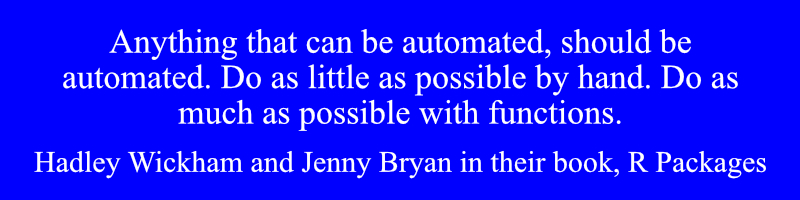
\includegraphics{_book/images/automate_as_much_as_possible.jpg}
\caption{Automate as much as
possible}
\end{figure}

\section{Principle: ``Is this my very best work?''}\label{principle-is-this-my-very-best-work}

This is your best work to build ensembles at this stage of your skills.
We are going to make a number of improvements to the solutions we see
here, so our final result will be much stronger than what we have here
so far. Always strive to do your very best work, without any excuses.

\section{``Where do I get help with errors or warnings?''}\label{where-do-i-get-help-with-errors-or-warnings}

It is extremely useful to check if your code returns any errors or
warnings, and fix those as fast as possible. There are numerous sites to
help address errors in your code:

\url{https://stackoverflow.com}

\url{https://forum.posit.co}

\url{https://www.r-project.org/help.html}

\section{Is there an easy way to save all trained models?}\label{is-there-an-easy-way-to-save-all-trained-models}

Absolutely! We will simply add the code at the end of this section that
saves the four trained models (linear, tree, ensemble\_linear and
ensemble\_tree), as follows:

\begin{Shaded}
\begin{Highlighting}[]
\FunctionTok{library}\NormalTok{(MASS)}
\FunctionTok{library}\NormalTok{(Metrics)}
\FunctionTok{library}\NormalTok{(tree)}

\NormalTok{ensemble\_lm\_rmse }\OtherTok{\textless{}{-}} \DecValTok{0}
\NormalTok{ensemble\_tree\_rmse }\OtherTok{\textless{}{-}} \DecValTok{0}

\ControlFlowTok{for}\NormalTok{ (i }\ControlFlowTok{in} \DecValTok{1}\SpecialCharTok{:}\DecValTok{100}\NormalTok{) \{}

\CommentTok{\# Fit the linear model with randomized data}

\NormalTok{df }\OtherTok{\textless{}{-}}\NormalTok{ df[}\FunctionTok{sample}\NormalTok{(}\FunctionTok{nrow}\NormalTok{(df)),] }\CommentTok{\# Randomize the rows before the analysis}

\NormalTok{train }\OtherTok{\textless{}{-}}\NormalTok{ df[}\DecValTok{1}\SpecialCharTok{:}\DecValTok{400}\NormalTok{, ]}
\NormalTok{test }\OtherTok{\textless{}{-}}\NormalTok{ df[}\DecValTok{401}\SpecialCharTok{:}\DecValTok{505}\NormalTok{, ]}

\NormalTok{Boston\_lm }\OtherTok{\textless{}{-}} \FunctionTok{lm}\NormalTok{(medv }\SpecialCharTok{\textasciitilde{}}\NormalTok{ ., }\AttributeTok{data =}\NormalTok{ train)}

\NormalTok{Boston\_lm\_predictions }\OtherTok{\textless{}{-}} \FunctionTok{predict}\NormalTok{(}\AttributeTok{object =}\NormalTok{ Boston\_lm, }\AttributeTok{newdata =}\NormalTok{ test)}

\CommentTok{\# Let\textquotesingle{}s have a quick look at the linear model predictions:}

\FunctionTok{head}\NormalTok{(Boston\_lm\_predictions)}

\CommentTok{\# Let\textquotesingle{}s calculate the root mean squared error rate of the predictions:}

\NormalTok{Boston\_linear\_rmse[i] }\OtherTok{\textless{}{-}}\NormalTok{ Metrics}\SpecialCharTok{::}\FunctionTok{rmse}\NormalTok{(}\AttributeTok{actual =}\NormalTok{ test}\SpecialCharTok{$}\NormalTok{medv, }\AttributeTok{predicted =}\NormalTok{ Boston\_lm\_predictions) }
\NormalTok{Boston\_linear\_rmse\_mean }\OtherTok{\textless{}{-}} \FunctionTok{mean}\NormalTok{(Boston\_linear\_rmse)}

\CommentTok{\# Let\textquotesingle{}s use tree models}

\NormalTok{Boston\_tree }\OtherTok{\textless{}{-}} \FunctionTok{tree}\NormalTok{(medv }\SpecialCharTok{\textasciitilde{}}\NormalTok{ ., }\AttributeTok{data =}\NormalTok{ train)}

\NormalTok{Boston\_tree\_predictions }\OtherTok{\textless{}{-}} \FunctionTok{predict}\NormalTok{(}\AttributeTok{object =}\NormalTok{ Boston\_tree, }\AttributeTok{newdata =}\NormalTok{ test)}

\CommentTok{\# Let\textquotesingle{}s have a quick look at the tree model predictions:}

\FunctionTok{head}\NormalTok{(Boston\_tree\_predictions)}

\CommentTok{\# Let\textquotesingle{}s calculate the root mean squared error rate of the predictions:}

\NormalTok{Boston\_tree\_rmse[i] }\OtherTok{\textless{}{-}}\NormalTok{ Metrics}\SpecialCharTok{::}\FunctionTok{rmse}\NormalTok{(}\AttributeTok{actual =}\NormalTok{ test}\SpecialCharTok{$}\NormalTok{medv, }\AttributeTok{predicted =}\NormalTok{ Boston\_tree\_predictions) }
\NormalTok{Boston\_tree\_rmse\_mean }\OtherTok{\textless{}{-}} \FunctionTok{mean}\NormalTok{(Boston\_tree\_rmse)}

\NormalTok{ensemble }\OtherTok{\textless{}{-}} \FunctionTok{data.frame}\NormalTok{( }\StringTok{\textquotesingle{}linear\textquotesingle{}} \OtherTok{=}\NormalTok{ Boston\_lm\_predictions, }\StringTok{\textquotesingle{}tree\textquotesingle{}} \OtherTok{=}\NormalTok{ Boston\_tree\_predictions, }\StringTok{\textquotesingle{}y\_ensemble\textquotesingle{}} \OtherTok{=}\NormalTok{ test}\SpecialCharTok{$}\NormalTok{medv )}

\NormalTok{ensemble }\OtherTok{\textless{}{-}}\NormalTok{ ensemble[}\FunctionTok{sample}\NormalTok{(}\FunctionTok{nrow}\NormalTok{(ensemble)), ] }\CommentTok{\# Randomizes the rows of the ensemble}

\NormalTok{ensemble\_train }\OtherTok{\textless{}{-}}\NormalTok{ ensemble[}\DecValTok{1}\SpecialCharTok{:}\DecValTok{60}\NormalTok{, ]}

\NormalTok{ensemble\_test }\OtherTok{\textless{}{-}}\NormalTok{ ensemble[}\DecValTok{61}\SpecialCharTok{:}\DecValTok{105}\NormalTok{, ]}

\CommentTok{\# Ensemble linear modeling}

\NormalTok{ensemble\_lm }\OtherTok{\textless{}{-}} \FunctionTok{lm}\NormalTok{(y\_ensemble }\SpecialCharTok{\textasciitilde{}}\NormalTok{ ., }\AttributeTok{data =}\NormalTok{ ensemble\_train)}

\CommentTok{\# Predictions for the ensemble linear model}

\NormalTok{ensemble\_prediction }\OtherTok{\textless{}{-}} \FunctionTok{predict}\NormalTok{(ensemble\_lm, }\AttributeTok{newdata =}\NormalTok{ ensemble\_test)}

\CommentTok{\# Root mean squared error for the ensemble linear model}

\NormalTok{ensemble\_lm\_rmse[i] }\OtherTok{\textless{}{-}}\NormalTok{ Metrics}\SpecialCharTok{::}\FunctionTok{rmse}\NormalTok{(}\AttributeTok{actual =}\NormalTok{ ensemble\_test}\SpecialCharTok{$}\NormalTok{y\_ensemble, }\AttributeTok{predicted =}\NormalTok{ ensemble\_prediction)}

\NormalTok{ensemble\_lm\_rmse\_mean }\OtherTok{\textless{}{-}} \FunctionTok{mean}\NormalTok{(ensemble\_lm\_rmse)}

\NormalTok{ensemble\_tree }\OtherTok{\textless{}{-}} \FunctionTok{tree}\NormalTok{(y\_ensemble }\SpecialCharTok{\textasciitilde{}}\NormalTok{ ., }\AttributeTok{data =}\NormalTok{ ensemble\_train)}

\NormalTok{ensemble\_tree\_predictions }\OtherTok{\textless{}{-}} \FunctionTok{predict}\NormalTok{(}\AttributeTok{object =}\NormalTok{ ensemble\_tree, }\AttributeTok{newdata =}\NormalTok{ ensemble\_test) }

\NormalTok{ensemble\_tree\_rmse[i] }\OtherTok{\textless{}{-}}\NormalTok{ Metrics}\SpecialCharTok{::}\FunctionTok{rmse}\NormalTok{(}\AttributeTok{actual =}\NormalTok{ ensemble\_test}\SpecialCharTok{$}\NormalTok{y\_ensemble, }\AttributeTok{predicted =}\NormalTok{ ensemble\_tree\_predictions)}

\NormalTok{ensemble\_tree\_rmse\_mean }\OtherTok{\textless{}{-}} \FunctionTok{mean}\NormalTok{(ensemble\_tree\_rmse)}

\NormalTok{results }\OtherTok{\textless{}{-}} \FunctionTok{list}\NormalTok{( }\StringTok{\textquotesingle{}Linear\textquotesingle{}} \OtherTok{=}\NormalTok{ Boston\_linear\_rmse\_mean, }\StringTok{\textquotesingle{}Trees\textquotesingle{}} \OtherTok{=}\NormalTok{ Boston\_tree\_rmse\_mean, }\StringTok{\textquotesingle{}Ensembles\_Linear\textquotesingle{}} \OtherTok{=}\NormalTok{ ensemble\_lm\_rmse\_mean, }\StringTok{\textquotesingle{}Ensemble\_Tree\textquotesingle{}} \OtherTok{=}\NormalTok{ ensemble\_tree\_rmse\_mean )}

\NormalTok{\}}

\NormalTok{results}
\CommentTok{\#\textgreater{} $Linear}
\CommentTok{\#\textgreater{} [1] 4.881756}
\CommentTok{\#\textgreater{} }
\CommentTok{\#\textgreater{} $Trees}
\CommentTok{\#\textgreater{} [1] 4.759513}
\CommentTok{\#\textgreater{} }
\CommentTok{\#\textgreater{} $Ensembles\_Linear}
\CommentTok{\#\textgreater{} [1] 4.200395}
\CommentTok{\#\textgreater{} }
\CommentTok{\#\textgreater{} $Ensemble\_Tree}
\CommentTok{\#\textgreater{} [1] 5.140953}
\end{Highlighting}
\end{Shaded}

\begin{Shaded}
\begin{Highlighting}[]
\FunctionTok{warnings}\NormalTok{()}
\end{Highlighting}
\end{Shaded}

\begin{Shaded}
\begin{Highlighting}[]

\NormalTok{Boston\_lm }\OtherTok{\textless{}{-}}\NormalTok{ Boston\_lm}
\NormalTok{Boston\_tree }\OtherTok{\textless{}{-}}\NormalTok{ Boston\_tree}
\NormalTok{ensemble\_lm }\OtherTok{\textless{}{-}}\NormalTok{ ensemble\_lm}
\NormalTok{ensemble\_tree }\OtherTok{\textless{}{-}}\NormalTok{ ensemble\_tree}
\end{Highlighting}
\end{Shaded}

\subsection{What about classification, logistic and time series data?}\label{what-about-classification-logistic-and-time-series-data}

In subsequent chapters we will do similar processes with classification,
logistic and time series data. It's possible to build ensembles with all
these types of data. The results are extremely similar to the results
we've seen here with numerical data: While the ensembles won't always
have the best results, it is best to have a diverse set of models and
ensembles to get the best possible results.

\subsection{Principle: Ensembles can work with many types of data, and we will do that in this book}\label{principle-ensembles-can-work-with-many-types-of-data-and-we-will-do-that-in-this-book}

\subsection{Can it make predictions on totally new data from the trained models---including the ensembles?}\label{can-it-make-predictions-on-totally-new-data-from-the-trained-modelsincluding-the-ensembles}

The solutions in this book are independent of the use of the data. We
will look at everything from housing prices to business analysis to HR
analytics to research in medicine. One of our later examples will do
exactly what this question is asking---build individual and ensemble
models from data, then use those pre-trained models to make predictions
on totally unseen data. You will develop this set of skills later in the
book, but it's a minor extension of what you're already seen and
completed.

\subsection{The way I was taught how to write code was totally wrong for me: The best way for me is to start at the end and work backward from there. Do not start coding looking for a solution, instead, start with the ending and work backwards from there.}\label{the-way-i-was-taught-how-to-write-code-was-totally-wrong-for-me-the-best-way-for-me-is-to-start-at-the-end-and-work-backward-from-there.-do-not-start-coding-looking-for-a-solution-instead-start-with-the-ending-and-work-backwards-from-there.}

\begin{figure}
\centering
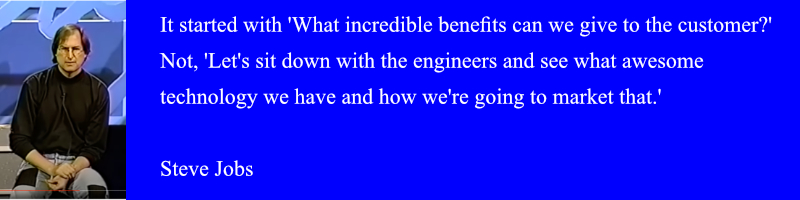
\includegraphics{_book/images/Steve Jobs.jpg}
\caption{Start at the end and work backwards}
\end{figure}

\href{https://www.youtube.com/watch?v=oeqPrUmVz-o}{Start at the end and work backwards from
there}

The biggest lesson for me in all of this work is how to make ensembles.
You've already seen some of the steps, and there are more results to
come. The second biggest lesson is that everything I was taught about
how to do data science and AI was backwards to what actually works for
me in real life. I've learned how I learn, and applied that skill
(learning how I learn) to a wide range of skills, including:

•~Running a multi-million dollar division of a Fortune 1000 company,
including full profit and loss responsibility

• Performing at a professional level on many musical instruments

•~Able to communicate in English, Spanish and sign language in a
professional setting

•~Earning the \#1 place on the annual undergradate university mathematics
competition---twice

• Completing a Master's degree in Guidance and Counseling, allowing me
to help many people in their path toward a healthier life

• Leader of the Oak Park, Illinois chapter of Amnesty International for
ten years, helping to release several Prisoners of Conscience

• President of the Chicago Apple User Group for ten years, helping many
people do extremely good work with their hardware and software

•~Leg press 1,000 pounds ten times in a row

•~Climbed a mountain in Colorado

• Completed multiple skydives (and looking forward to doing more)

The point here is that I have learned how I learn, and I've applied that
skill to many areas. When I started learning data science/AI/coding, it
was all very different from the way I was being creative my whole life.
The way that works for me is to start at the end, work backward from
there, and never give up. Maybe the best evidence of the success of this
method is this fact:

\textbf{When I started to write the code that led to the Ensembles package, I
followed those steps: Start at the end, work backward from there, and
never give up. I wound up writing an average of 1,000 lines of clean,
error free code per month for 15 months. The Ensembles package is around
15,000 lines of clean, error free code.}

I found my attitude was much more important than my skill set, by a long
shot.

\subsection{How I stuck with it all the way to the end: The best career advice I ever received was from a homeless man I never met, and answers the question of what most strongly predicts success.}\label{how-i-stuck-with-it-all-the-way-to-the-end-the-best-career-advice-i-ever-received-was-from-a-homeless-man-i-never-met-and-answers-the-question-of-what-most-strongly-predicts-success.}

\begin{figure}
\centering

\includegraphics{_book/images/Ashford_and_Simpson.png}
\caption{Ashford and Simpson}
\end{figure}

Ashford and Simpson

Learning about building ensembles will help you make more accurate
predictions. That's an extrdmely good skill to have in any setting. But
I found the most important thing to predict is success. This has been
studied, and there are quite a few good works on the subject, both
academic and for the general population.

My favorite career advice---which I listened to nearly every day as I
worked on the Ensembles project---is from a man who was homeless at the
time he came up with the words.

Nick Ashford was from Willow Run, Michigan. He moved to New York, hoping
to get into the entertainment world as a dancer. Unfortunately he ended
up homeless on the streets of New York. He slept on park benches, and
got food from soup kitchens.

He heard that the people at White Rock Baptist Church would feed him (a
homeless man) a normal meal, so Nick went there one Sunday morning. He
met the people, especially the choir members, and started working with
the piano player in the choir. Her name is Valerie Simpson.

Soon Nick and Valerie were writing songs for the church choir. Nick
mentioned that while he was homeless, he realized that New York wasn't
going to ``do me in''. He was determined. The words he put down say:

\textbf{Ain't no mountain high enough}

\textbf{Ain't no valley low enough}

\textbf{Ain't no river wide enough}

Valerie took those words, and set them to music. They sent that song to
Motown, who released it with Marvin Gaye and Tammy Terrell covering the
vocals. It was later re-done by Ashford and Simpson and Paul Riser, with
Diana Ross singing the lead.

Here is a short video that summarizes that experience, and concludes
with the finale of the 1970 version of the song. This attitude that
Ashford and Simpson expressed in song is extremely highly predictive of
success, no matter what the field of endeavor. I found this extremely
motivating, and used it to overcome any obstacles and challenges I had
while on the journey.

While I have the skill of knowing how I learn (which I will continue to
share with you in this book), this attitude of working no matter how
high the mountain or long the valley or wide the river, gives me the how
and the why to keep moving toward success, until that success is fully
achieved.

Later on we will look at how to make presentations, consider this as an
example of the level of quality that can be done:

\href{https://www.icloud.com/iclouddrive/002bNfVreagRYCYHAZ9GyQ02w\#Ain't\%5FNo\%5FMountain\%5FHigh\%5FEnough}{https://www.icloud.com/iclouddrive/002bNfVreagRYCYHAZ9GyQ02w\#Ain't\%5FNo\%5FMountain\%5FHigh\%5FEnough}

\subsection{Exercises:}\label{exercises}

\begin{enumerate}
\def\labelenumi{\arabic{enumi}.}
\tightlist
\item
  Find your data science Genesis. The data science idea that totally
  excites you and gets you out of bed every day. The idea that leads
  to the creation of many other ideas. The biggest and boldest dreams
  you can possibly have. The idea that is so strong that you have to
  do it. Not for yourself, but for the benefit of all who will use it
  and receive all the good it will create.
\item
  Keep a journal of your progress. It's much easier to see results
  over time when there is a record. Set the journal up today (or this
  week). I did not use Github as a journal. My journal was for crazy
  ideas, contradictory evidence, writing down my frustrations and
  successes, inspiration, the one next thing I worked on, and having a
  rock solid record of the path to success. Seeing the path I
  traversed was a huge motivation to finishing the project.
\item
  Do your best to add journal entries to your regular schedule.
\item
  Make an ensemble using the Boston Housing data set. Model any of the
  other 13 columns of data, not the median value of the home (14th
  column) which we have been working on in this chapter.
\item
  Start planning for your comprehensive project. What types of data
  are you most interested in? What patterns would you like to
  discover? Begin looking online now for possible data sets, and so a
  little basic research. More examples will be provided as we get
  closer to that section of the book.
\end{enumerate}

\chapter{Numerical data: How to make 23 individual models, and basic skills with functions}\label{numerical-data-how-to-make-23-individual-models-and-basic-skills-with-functions}

This is where we will begin building the skills to make ensembles of
models of numerical data. However, this is going to be much easier than
it might appear at first. Let's see how we can make this as easy as
possible.

How to work backwards and make the function we need: Start from the end

We are going to start at the ending, not at the beginning, and work
backwards from there. This method is much, much easier than working
forward, as you will see throughout this book. While it might be a
little uncomfortable at first, this skill will allow you to complete
your work at a faster rate than if you work forward.

We'll use the Boston Housing data set, and we'll start with the Bagged
Random Forest function. For now we're only going to work with one
function, to keep everything simple. In essence, we are going to run
this like an assembly line.

We want the ending to be the error rate by model. Virtually any customer
you work with is going to want to know, ``How accurate is it?'' That's our
starting point.

How do we determine model accuracy? We already did this in the previous
chapter, finding the root mean squared error for the individual models
and the ensemble models. We're going to do the same steps here, so the
process is familiar to you.

To get the error rate by model on the holdout data sets (test and
validation), we're going to need a model (Bagged Random Forest in this
first example), fit to the training data, and use that model to make
predictions on the test data. We can then measure the error in the
predictions, just as we did before. These steps should be familiar to
you. If not, please re-read the previous chapter.

But what do we need to complete those steps? We're going to have to go
backward (a little) and make a function that will allow us to work with
any data set.

What does our function need? Let's make a list:

\begin{itemize}
\item
  The data (such as Boston housing)
\item
  Column number (such as 14, the median value of the property)
\item
  Train amount
\item
  Test amount
\item
  Validation amount
\item
  Number of times to resample
\end{itemize}

One of the key steps here is to change the name of the target variable
to y. The initial name could be nearly anything, but this method changes
the name of the target variable to y. This allows us to make one small
change that will allow this to be the easiest possible solution:

\subsection{All our models will be structured the same way: y \textasciitilde{} ., data = train}\label{all-our-models-will-be-structured-the-same-way-y-.-data-train}

This means that y (our target value) is a function of the other
features, and the data set is the training data set. While there will be
some variations on this in our 27 models, the basic structure is the
same.

\subsection{Having the same structure for all the models makes it much easier to build, debug, and deploy the completed models.}\label{having-the-same-structure-for-all-the-models-makes-it-much-easier-to-build-debug-and-deploy-the-completed-models.}

Then we only need to start with our initial values, and it will run.

One extremely nice part about creating models this way is the enormous
efficiency it gives us. Once we have the Bagged Random Forest model
working, we will be able to use very similar (and identical in many
cases!) processes with other models (such as Support Vector Machines).

The rock solid foundation we lay at the beginning will allow us to have
a smooth and easy experience once the foundation is solid and we use it
to build more models. The other models will mainly be almost exact
duplicates of our fist example.'

Here are the steps we will follow:

\begin{itemize}
\item
  Load the library
\item
  Set initial values to 0
\item
  Create the function
\item
  Set up random resampling
\item
  Break the data into train and test
\item
  Fit the model on the training data, make predictions and measure
  error on the test data
\item
  Return the results
\item
  Check for errors or warnings
\item
  Test on a different data set
\end{itemize}

\subsection{Exercise: Re-read the steps above how we will work backwards to come up with the function we need.}\label{exercise-re-read-the-steps-above-how-we-will-work-backwards-to-come-up-with-the-function-we-need.}

\begin{Shaded}
\begin{Highlighting}[]
\FunctionTok{library}\NormalTok{(e1071) }\CommentTok{\# will allow us to use a tuned random forest model}
\FunctionTok{library}\NormalTok{(Metrics) }\CommentTok{\# Will allow us to calculate the root mean squared error}
\FunctionTok{library}\NormalTok{(randomForest) }\CommentTok{\# To use the random forest function}
\CommentTok{\#\textgreater{} randomForest 4.7{-}1.1}
\CommentTok{\#\textgreater{} Type rfNews() to see new features/changes/bug fixes.}
\end{Highlighting}
\end{Shaded}

\begin{Shaded}
\begin{Highlighting}[]
\FunctionTok{library}\NormalTok{(tidyverse) }\CommentTok{\# Amazing set of tools for data science}
\CommentTok{\#\textgreater{} {-}{-} Attaching core tidyverse packages {-}{-}{-}{-} tidyverse 2.0.0 {-}{-}}
\CommentTok{\#\textgreater{} v dplyr     1.1.4     v readr     2.1.5}
\CommentTok{\#\textgreater{} v forcats   1.0.0     v stringr   1.5.1}
\CommentTok{\#\textgreater{} v ggplot2   3.5.1     v tibble    3.2.1}
\CommentTok{\#\textgreater{} v lubridate 1.9.3     v tidyr     1.3.1}
\CommentTok{\#\textgreater{} v purrr     1.0.2}
\CommentTok{\#\textgreater{} {-}{-} Conflicts {-}{-}{-}{-}{-}{-}{-}{-}{-}{-}{-}{-}{-}{-}{-}{-}{-}{-}{-}{-}{-}{-} tidyverse\_conflicts() {-}{-}}
\CommentTok{\#\textgreater{} x dplyr::combine()  masks randomForest::combine()}
\CommentTok{\#\textgreater{} x dplyr::filter()   masks stats::filter()}
\CommentTok{\#\textgreater{} x dplyr::lag()      masks stats::lag()}
\CommentTok{\#\textgreater{} x ggplot2::margin() masks randomForest::margin()}
\CommentTok{\#\textgreater{} i Use the conflicted package (\textless{}http://conflicted.r{-}lib.org/\textgreater{}) to force all conflicts to become errors}
\end{Highlighting}
\end{Shaded}

\begin{Shaded}
\begin{Highlighting}[]
\CommentTok{\# Set initial values to 0. The function will return an error if any of these are left out.}

\NormalTok{bag\_rf\_holdout\_RMSE }\OtherTok{\textless{}{-}} \DecValTok{0}
\NormalTok{bag\_rf\_holdout\_RMSE\_mean }\OtherTok{\textless{}{-}} \DecValTok{0}
\NormalTok{bag\_rf\_train\_RMSE }\OtherTok{\textless{}{-}} \DecValTok{0}
\NormalTok{bag\_rf\_test\_RMSE }\OtherTok{\textless{}{-}} \DecValTok{0}
\NormalTok{bag\_rf\_validation\_RMSE }\OtherTok{\textless{}{-}} \DecValTok{0}
\end{Highlighting}
\end{Shaded}

\begin{Shaded}
\begin{Highlighting}[]

\CommentTok{\# Define the function}

\NormalTok{numerical\_1 }\OtherTok{\textless{}{-}} \ControlFlowTok{function}\NormalTok{(data, colnum, train\_amount, test\_amount, numresamples)\{}

\CommentTok{\#Set up random resampling}

\ControlFlowTok{for}\NormalTok{ (i }\ControlFlowTok{in} \DecValTok{1}\SpecialCharTok{:}\NormalTok{numresamples) \{}

\CommentTok{\# Changes the name of the target column to y}
\NormalTok{y }\OtherTok{\textless{}{-}} \DecValTok{0}
\FunctionTok{colnames}\NormalTok{(data)[colnum] }\OtherTok{\textless{}{-}} \StringTok{"y"}

\CommentTok{\# Moves the target column to the last column on the right}
\NormalTok{df }\OtherTok{\textless{}{-}}\NormalTok{ data }\SpecialCharTok{\%\textgreater{}\%}\NormalTok{ dplyr}\SpecialCharTok{::}\FunctionTok{relocate}\NormalTok{(y, }\AttributeTok{.after =} \FunctionTok{last\_col}\NormalTok{())}
\NormalTok{df }\OtherTok{\textless{}{-}}\NormalTok{ df[}\FunctionTok{sample}\NormalTok{(}\FunctionTok{nrow}\NormalTok{(df)), ] }\CommentTok{\# randomizes the rows}

\CommentTok{\#Breaks the data into train and test sets}
\NormalTok{idx }\OtherTok{\textless{}{-}} \FunctionTok{sample}\NormalTok{(}\FunctionTok{seq}\NormalTok{(}\DecValTok{1}\NormalTok{, }\DecValTok{2}\NormalTok{), }\AttributeTok{size =} \FunctionTok{nrow}\NormalTok{(df), }\AttributeTok{replace =} \ConstantTok{TRUE}\NormalTok{, }\AttributeTok{prob =} \FunctionTok{c}\NormalTok{(train\_amount, test\_amount))}
\NormalTok{train }\OtherTok{\textless{}{-}}\NormalTok{ df[idx }\SpecialCharTok{==} \DecValTok{1}\NormalTok{, ]}
\NormalTok{test }\OtherTok{\textless{}{-}}\NormalTok{ df[idx }\SpecialCharTok{==} \DecValTok{2}\NormalTok{, ]}

\CommentTok{\# Fit the model to the training data, make predictions on the testing data, then calculate the error rates on the testing data sets.}
\NormalTok{bag\_rf\_train\_fit }\OtherTok{\textless{}{-}}\NormalTok{ e1071}\SpecialCharTok{::}\FunctionTok{tune.randomForest}\NormalTok{(}\AttributeTok{x =}\NormalTok{ train, }\AttributeTok{y =}\NormalTok{ train}\SpecialCharTok{$}\NormalTok{y, }\AttributeTok{mtry =} \FunctionTok{ncol}\NormalTok{(train) }\SpecialCharTok{{-}} \DecValTok{1}\NormalTok{)}
\NormalTok{bag\_rf\_train\_RMSE[i] }\OtherTok{\textless{}{-}}\NormalTok{ Metrics}\SpecialCharTok{::}\FunctionTok{rmse}\NormalTok{(}\AttributeTok{actual =}\NormalTok{ train}\SpecialCharTok{$}\NormalTok{y, }\AttributeTok{predicted =} \FunctionTok{predict}\NormalTok{( }\AttributeTok{object =}\NormalTok{ bag\_rf\_train\_fit}\SpecialCharTok{$}\NormalTok{best.model, }\AttributeTok{newdata =}\NormalTok{ train))}
\NormalTok{bag\_rf\_train\_RMSE\_mean }\OtherTok{\textless{}{-}} \FunctionTok{mean}\NormalTok{(bag\_rf\_train\_RMSE)}
\NormalTok{bag\_rf\_test\_RMSE[i] }\OtherTok{\textless{}{-}}\NormalTok{ Metrics}\SpecialCharTok{::}\FunctionTok{rmse}\NormalTok{(}\AttributeTok{actual =}\NormalTok{ test}\SpecialCharTok{$}\NormalTok{y, }\AttributeTok{predicted =} \FunctionTok{predict}\NormalTok{( }\AttributeTok{object =}\NormalTok{ bag\_rf\_train\_fit}\SpecialCharTok{$}\NormalTok{best.model, }\AttributeTok{newdata =}\NormalTok{ test))}
\NormalTok{bag\_rf\_test\_RMSE\_mean }\OtherTok{\textless{}{-}} \FunctionTok{mean}\NormalTok{(bag\_rf\_test\_RMSE)}

\CommentTok{\# Itemize the error on the holdout data sets, and calculate the mean of the results}
\NormalTok{bag\_rf\_holdout\_RMSE[i] }\OtherTok{\textless{}{-}} \FunctionTok{mean}\NormalTok{(bag\_rf\_test\_RMSE\_mean)}
\NormalTok{bag\_rf\_holdout\_RMSE\_mean }\OtherTok{\textless{}{-}} \FunctionTok{mean}\NormalTok{(}\FunctionTok{c}\NormalTok{(bag\_rf\_holdout\_RMSE))}

\CommentTok{\# These are the predictions we will need when we make the ensembles}
\NormalTok{bag\_rf\_test\_predict\_value }\OtherTok{\textless{}{-}} \FunctionTok{as.numeric}\NormalTok{(}\FunctionTok{predict}\NormalTok{(}\AttributeTok{object =}\NormalTok{ bag\_rf\_train\_fit}\SpecialCharTok{$}\NormalTok{best.model, }\AttributeTok{newdata =}\NormalTok{ test))}


\CommentTok{\#Return the mean of the results to the user}

\FunctionTok{return}\NormalTok{(bag\_rf\_holdout\_RMSE\_mean)}
\NormalTok{\} }\CommentTok{\# closing brace for numresamples}
\NormalTok{\} }\CommentTok{\# closing brace for numerical\_1 function}

\CommentTok{\# Here is our first numerical function in actual use. We will use 25 resamples}

\FunctionTok{numerical\_1}\NormalTok{(}\AttributeTok{data =}\NormalTok{ MASS}\SpecialCharTok{::}\NormalTok{Boston, }\AttributeTok{colnum =} \DecValTok{14}\NormalTok{, }\AttributeTok{train\_amount =} \FloatTok{0.60}\NormalTok{, }\AttributeTok{test\_amount =} \FloatTok{0.40}\NormalTok{, }\AttributeTok{numresamples =} \DecValTok{25}\NormalTok{)}
\CommentTok{\#\textgreater{} [1] 0.2555779}
\end{Highlighting}
\end{Shaded}

\begin{Shaded}
\begin{Highlighting}[]
\FunctionTok{warnings}\NormalTok{() }\CommentTok{\# no warnings, the best possible result}
\end{Highlighting}
\end{Shaded}

Exercise: Try it yourself: Change the values of train, test and
validation, and the number of resamples. See how those change the
result.

One of your own: Find any numerical data set, and make a bagged random
forest function for that data set. (For example, you may use the Auto
data set in the ISLR package. You will need to remove the last column,
vehicle name. Model mpg as a function of the other features using the
Bagged Random Forest function, but any numerical data set will work).

Post: Share on social your first results making a numerical function
(screen shot/video optional at this stage, we will be learning how to do
those later)

For example, ``Did my first data science function building up to making
ensembles later on. Got everything to run, no errors. \#AIEnsembles''

Now we will build the remaining 22 models for numerical data. They are
all built using the same structure, on the same foundation.

Now that we know how to build a basic function, let's build the 22 other
sets of tools we will need to make our ensemble, starting with bagging:

\subsection{Bagging (bootstrap aggregating)}\label{bagging-bootstrap-aggregating}

\begin{Shaded}
\begin{Highlighting}[]
\FunctionTok{library}\NormalTok{(ipred) }\CommentTok{\#for the bagging function}

\CommentTok{\# Set initial values to 0}
\NormalTok{bagging\_train\_RMSE }\OtherTok{\textless{}{-}} \DecValTok{0}
\NormalTok{bagging\_test\_RMSE }\OtherTok{\textless{}{-}} \DecValTok{0}
\NormalTok{bagging\_validation\_RMSE }\OtherTok{\textless{}{-}} \DecValTok{0}
\NormalTok{bagging\_holdout\_RMSE }\OtherTok{\textless{}{-}} \DecValTok{0}
\NormalTok{bagging\_test\_predict\_value }\OtherTok{\textless{}{-}} \DecValTok{0}
\NormalTok{bagging\_validation\_predict\_value }\OtherTok{\textless{}{-}} \DecValTok{0}

\CommentTok{\#Create the function:}

\NormalTok{bagging\_1 }\OtherTok{\textless{}{-}} \ControlFlowTok{function}\NormalTok{(data, colnum, train\_amount, test\_amount, validation\_amount, numresamples)\{}

\CommentTok{\#Set up random resampling}
\ControlFlowTok{for}\NormalTok{ (i }\ControlFlowTok{in} \DecValTok{1}\SpecialCharTok{:}\NormalTok{numresamples) \{}

\CommentTok{\#Changes the name of the target column to y}
\NormalTok{y }\OtherTok{\textless{}{-}} \DecValTok{0}
\FunctionTok{colnames}\NormalTok{(data)[colnum] }\OtherTok{\textless{}{-}} \StringTok{"y"}

\CommentTok{\# Moves the target column to the last column on the right}
\NormalTok{df }\OtherTok{\textless{}{-}}\NormalTok{ data }\SpecialCharTok{\%\textgreater{}\%}\NormalTok{ dplyr}\SpecialCharTok{::}\FunctionTok{relocate}\NormalTok{(y, }\AttributeTok{.after =} \FunctionTok{last\_col}\NormalTok{()) }\CommentTok{\# Moves the target column to the last column on the right df \textless{}{-} df[sample(nrow(df)), ] \# randomizes the rows}

\CommentTok{\# Breaks the data into train and test sets}

\NormalTok{idx }\OtherTok{\textless{}{-}} \FunctionTok{sample}\NormalTok{(}\FunctionTok{seq}\NormalTok{(}\DecValTok{1}\NormalTok{, }\DecValTok{2}\NormalTok{), }\AttributeTok{size =} \FunctionTok{nrow}\NormalTok{(df), }\AttributeTok{replace =} \ConstantTok{TRUE}\NormalTok{, }\AttributeTok{prob =} \FunctionTok{c}\NormalTok{(train\_amount, test\_amount))}
\NormalTok{train }\OtherTok{\textless{}{-}}\NormalTok{ df[idx }\SpecialCharTok{==} \DecValTok{1}\NormalTok{, ]}
\NormalTok{test }\OtherTok{\textless{}{-}}\NormalTok{ df[idx }\SpecialCharTok{==} \DecValTok{2}\NormalTok{, ]}

\CommentTok{\# Fit the model to the training data, calculate error, make predictions on the holdout data}

\NormalTok{bagging\_train\_fit }\OtherTok{\textless{}{-}}\NormalTok{ ipred}\SpecialCharTok{::}\FunctionTok{bagging}\NormalTok{(}\AttributeTok{formula =}\NormalTok{ y }\SpecialCharTok{\textasciitilde{}}\NormalTok{ ., }\AttributeTok{data =}\NormalTok{ train)}
\NormalTok{bagging\_train\_RMSE[i] }\OtherTok{\textless{}{-}}\NormalTok{ Metrics}\SpecialCharTok{::}\FunctionTok{rmse}\NormalTok{(}\AttributeTok{actual =}\NormalTok{ train}\SpecialCharTok{$}\NormalTok{y, }\AttributeTok{predicted =} \FunctionTok{predict}\NormalTok{(}\AttributeTok{object =}\NormalTok{ bagging\_train\_fit, }\AttributeTok{newdata =}\NormalTok{ train))}
\NormalTok{bagging\_train\_RMSE\_mean }\OtherTok{\textless{}{-}} \FunctionTok{mean}\NormalTok{(bagging\_train\_RMSE)}
\NormalTok{bagging\_test\_RMSE[i] }\OtherTok{\textless{}{-}}\NormalTok{ Metrics}\SpecialCharTok{::}\FunctionTok{rmse}\NormalTok{(}\AttributeTok{actual =}\NormalTok{ test}\SpecialCharTok{$}\NormalTok{y, }\AttributeTok{predicted =} \FunctionTok{predict}\NormalTok{(}\AttributeTok{object =}\NormalTok{ bagging\_train\_fit, }\AttributeTok{newdata =}\NormalTok{ test))}
\NormalTok{bagging\_test\_RMSE\_mean }\OtherTok{\textless{}{-}} \FunctionTok{mean}\NormalTok{(bagging\_test\_RMSE)}
\NormalTok{bagging\_holdout\_RMSE[i] }\OtherTok{\textless{}{-}} \FunctionTok{mean}\NormalTok{(bagging\_test\_RMSE\_mean)}
\NormalTok{bagging\_holdout\_RMSE\_mean }\OtherTok{\textless{}{-}} \FunctionTok{mean}\NormalTok{(bagging\_holdout\_RMSE)}
\NormalTok{y\_hat\_bagging }\OtherTok{\textless{}{-}} \FunctionTok{c}\NormalTok{(bagging\_test\_predict\_value)}

\FunctionTok{return}\NormalTok{(bagging\_holdout\_RMSE\_mean)}

\NormalTok{\} }\CommentTok{\# closing braces for the resampling function}
\NormalTok{\} }\CommentTok{\# closing braces for the bagging function}

\CommentTok{\# Test the function:}
\FunctionTok{bagging\_1}\NormalTok{(}\AttributeTok{data =}\NormalTok{ MASS}\SpecialCharTok{::}\NormalTok{Boston, }\AttributeTok{colnum =} \DecValTok{14}\NormalTok{, }\AttributeTok{train\_amount =} \FloatTok{0.60}\NormalTok{, }\AttributeTok{test\_amount =} \FloatTok{0.20}\NormalTok{, }\AttributeTok{numresamples =} \DecValTok{25}\NormalTok{)}
\CommentTok{\#\textgreater{} [1] 3.477499}
\end{Highlighting}
\end{Shaded}

\begin{Shaded}
\begin{Highlighting}[]
\FunctionTok{warnings}\NormalTok{() }\CommentTok{\# no warnings}
\end{Highlighting}
\end{Shaded}

\subsection{BayesGLM}\label{bayesglm}

\begin{Shaded}
\begin{Highlighting}[]
\FunctionTok{library}\NormalTok{(arm) }\CommentTok{\# to use bayesglm function}
\CommentTok{\#\textgreater{} Loading required package: MASS}
\CommentTok{\#\textgreater{} }
\CommentTok{\#\textgreater{} Attaching package: \textquotesingle{}MASS\textquotesingle{}}
\CommentTok{\#\textgreater{} The following object is masked from \textquotesingle{}package:dplyr\textquotesingle{}:}
\CommentTok{\#\textgreater{} }
\CommentTok{\#\textgreater{}     select}
\CommentTok{\#\textgreater{} Loading required package: Matrix}
\CommentTok{\#\textgreater{} }
\CommentTok{\#\textgreater{} Attaching package: \textquotesingle{}Matrix\textquotesingle{}}
\CommentTok{\#\textgreater{} The following objects are masked from \textquotesingle{}package:tidyr\textquotesingle{}:}
\CommentTok{\#\textgreater{} }
\CommentTok{\#\textgreater{}     expand, pack, unpack}
\CommentTok{\#\textgreater{} Loading required package: lme4}
\CommentTok{\#\textgreater{} }
\CommentTok{\#\textgreater{} arm (Version 1.14{-}4, built: 2024{-}4{-}1)}
\CommentTok{\#\textgreater{} Working directory is /Users/russellconte/Library/Mobile Documents/com\textasciitilde{}apple\textasciitilde{}CloudDocs/Documents/Machine Learning templates in R/Ensembles\_Book}
\end{Highlighting}
\end{Shaded}

\begin{Shaded}
\begin{Highlighting}[]

\CommentTok{\# Set initial values to 0}
\NormalTok{bayesglm\_train\_RMSE }\OtherTok{\textless{}{-}} \DecValTok{0}
\NormalTok{bayesglm\_test\_RMSE }\OtherTok{\textless{}{-}} \DecValTok{0}
\NormalTok{bayesglm\_validation\_RMSE }\OtherTok{\textless{}{-}} \DecValTok{0}
\NormalTok{bayesglm\_holdout\_RMSE }\OtherTok{\textless{}{-}} \DecValTok{0}
\NormalTok{bayesglm\_test\_predict\_value }\OtherTok{\textless{}{-}} \DecValTok{0}
\NormalTok{bayesglm\_validation\_predict\_value }\OtherTok{\textless{}{-}} \DecValTok{0}

\CommentTok{\# Create the function:}
\NormalTok{bayesglm\_1 }\OtherTok{\textless{}{-}} \ControlFlowTok{function}\NormalTok{(data, colnum, train\_amount, test\_amount, numresamples)\{}

\CommentTok{\#Set up random resampling}
\ControlFlowTok{for}\NormalTok{ (i }\ControlFlowTok{in} \DecValTok{1}\SpecialCharTok{:}\NormalTok{numresamples) \{}

\CommentTok{\#Changes the name of the target column to y}
\NormalTok{y }\OtherTok{\textless{}{-}} \DecValTok{0}
\FunctionTok{colnames}\NormalTok{(data)[colnum] }\OtherTok{\textless{}{-}} \StringTok{"y"}

\CommentTok{\#Moves the target column to the last column on the right}
\NormalTok{df }\OtherTok{\textless{}{-}}\NormalTok{ data }\SpecialCharTok{\%\textgreater{}\%}\NormalTok{ dplyr}\SpecialCharTok{::}\FunctionTok{relocate}\NormalTok{(y, }\AttributeTok{.after =} \FunctionTok{last\_col}\NormalTok{()) }\CommentTok{\# Moves the target column to the last column on the right df \textless{}{-} df[sample(nrow(df)), ] \# randomizes the rows}

\CommentTok{\#Breaks the data into train, test and validation sets}
\NormalTok{idx }\OtherTok{\textless{}{-}} \FunctionTok{sample}\NormalTok{(}\FunctionTok{seq}\NormalTok{(}\DecValTok{1}\NormalTok{, }\DecValTok{2}\NormalTok{), }\AttributeTok{size =} \FunctionTok{nrow}\NormalTok{(df), }\AttributeTok{replace =} \ConstantTok{TRUE}\NormalTok{, }\AttributeTok{prob =} \FunctionTok{c}\NormalTok{(train\_amount, test\_amount))}
\NormalTok{train }\OtherTok{\textless{}{-}}\NormalTok{ df[idx }\SpecialCharTok{==} \DecValTok{1}\NormalTok{, ]}
\NormalTok{test }\OtherTok{\textless{}{-}}\NormalTok{ df[idx }\SpecialCharTok{==} \DecValTok{2}\NormalTok{, ]}

\NormalTok{bayesglm\_train\_fit }\OtherTok{\textless{}{-}}\NormalTok{ arm}\SpecialCharTok{::}\FunctionTok{bayesglm}\NormalTok{(y }\SpecialCharTok{\textasciitilde{}}\NormalTok{ ., }\AttributeTok{data =}\NormalTok{ train, }\AttributeTok{family =} \FunctionTok{gaussian}\NormalTok{(}\AttributeTok{link =} \StringTok{"identity"}\NormalTok{))}
\NormalTok{bayesglm\_train\_RMSE[i] }\OtherTok{\textless{}{-}}\NormalTok{ Metrics}\SpecialCharTok{::}\FunctionTok{rmse}\NormalTok{(}\AttributeTok{actual =}\NormalTok{ train}\SpecialCharTok{$}\NormalTok{y, }\AttributeTok{predicted =} \FunctionTok{predict}\NormalTok{(}\AttributeTok{object =}\NormalTok{ bayesglm\_train\_fit, }\AttributeTok{newdata =}\NormalTok{ train))}
\NormalTok{bayesglm\_train\_RMSE\_mean }\OtherTok{\textless{}{-}} \FunctionTok{mean}\NormalTok{(bayesglm\_train\_RMSE)}
\NormalTok{bayesglm\_test\_RMSE[i] }\OtherTok{\textless{}{-}}\NormalTok{ Metrics}\SpecialCharTok{::}\FunctionTok{rmse}\NormalTok{(}\AttributeTok{actual =}\NormalTok{ test}\SpecialCharTok{$}\NormalTok{y, }\AttributeTok{predicted =} \FunctionTok{predict}\NormalTok{(}\AttributeTok{object =}\NormalTok{ bayesglm\_train\_fit, }\AttributeTok{newdata =}\NormalTok{ test))}
\NormalTok{bayesglm\_test\_RMSE\_mean }\OtherTok{\textless{}{-}} \FunctionTok{mean}\NormalTok{(bayesglm\_test\_RMSE) }
\NormalTok{y\_hat\_bayesglm }\OtherTok{\textless{}{-}} \FunctionTok{c}\NormalTok{(bayesglm\_test\_predict\_value)}

\FunctionTok{return}\NormalTok{(bayesglm\_test\_RMSE\_mean)}

\NormalTok{\} }\CommentTok{\# closing braces for resampling}
\NormalTok{\} }\CommentTok{\# closing braces for the function}

\FunctionTok{bayesglm\_1}\NormalTok{(}\AttributeTok{data =}\NormalTok{ MASS}\SpecialCharTok{::}\NormalTok{Boston, }\AttributeTok{colnum =} \DecValTok{14}\NormalTok{, }\AttributeTok{train\_amount =} \FloatTok{0.60}\NormalTok{, }\AttributeTok{test\_amount =} \FloatTok{0.20}\NormalTok{, }\AttributeTok{numresamples =} \DecValTok{25}\NormalTok{)}
\CommentTok{\#\textgreater{} [1] 4.938509}
\end{Highlighting}
\end{Shaded}

\begin{Shaded}
\begin{Highlighting}[]
\FunctionTok{warnings}\NormalTok{() }\CommentTok{\# no warnings}
\end{Highlighting}
\end{Shaded}

BayesRNN

\{r BayesRNN model for numerical data\}

library(brnn) \# so we can use the BayesRNN function

\chapter{Set initial values to 0}\label{set-initial-values-to-0}

bayesrnn\_train\_RMSE \textless- 0 bayesrnn\_test\_RMSE \textless- 0
bayesrnn\_validation\_RMSE \textless- 0 bayesrnn\_holdout\_RMSE \textless- 0
bayesrnn\_test\_predict\_value \textless- 0 bayesrnn\_validation\_predict\_value \textless-
0

\chapter{Create the function:}\label{create-the-function}

bayesrnn \textless- function(data, colnum, train\_amount, test\_amount,
validation\_amount, numresamples)\{

\chapter{Set up random resampling}\label{set-up-random-resampling}

for (i in 1:numresamples) \{

\chapter{Changes the name of the target column to y}\label{changes-the-name-of-the-target-column-to-y}

y \textless- 0 colnames(data){[}colnum{]} \textless- ``y''

\chapter{Moves the target column to the last column on the right}\label{moves-the-target-column-to-the-last-column-on-the-right}

df \textless- data \%\textgreater\% dplyr::relocate(y, .after = last\_col()) \# Moves the
target column to the last column on the right df \textless-
df{[}sample(nrow(df)), {]} \# randomizes the rows

\chapter{Breaks the data into train, test and validation sets}\label{breaks-the-data-into-train-test-and-validation-sets}

idx \textless- sample(seq(1, 3), size = nrow(df), replace = TRUE, prob =
c(train\_amount, test\_amount, validation\_amount)) train \textless- df{[}idx == 1,{]} test \textless- df{[}idx == 2, {]} validation \textless- df{[}idx == 3, {]}

bayesrnn\_train\_fit \textless- brnn::brnn(x = as.matrix(train), y = train\(y)
bayesrnn_train_RMSE[i] <- Metrics::rmse(actual = train\)y, predicted =
predict(object = bayesrnn\_train\_fit, newdata = train))
bayesrnn\_train\_RMSE\_mean \textless- mean(bayesrnn\_train\_RMSE)
bayesrnn\_test\_RMSE{[}i{]} \textless- Metrics::rmse(actual =
test\(y, predicted = predict(object = bayesrnn_train_fit, newdata = test))
bayesrnn_test_RMSE_mean <- mean(bayesrnn_test_RMSE)
bayesrnn_validation_RMSE[i] <- Metrics::rmse(actual = validation\)y,
predicted = predict(object = bayesrnn\_train\_fit, newdata = validation))
bayesrnn\_validation\_RMSE\_mean \textless- mean(bayesrnn\_validation\_RMSE)
bayesrnn\_holdout\_RMSE{[}i{]} \textless- mean(c(bayesrnn\_test\_RMSE\_mean,
bayesrnn\_validation\_RMSE\_mean)) bayesrnn\_holdout\_RMSE\_mean \textless-
mean(bayesrnn\_holdout\_RMSE)

bayesrnn\_test\_predict\_value \textless- as.numeric(predict(object =
bayesrnn\_train\_fit, newdata = test)) bayesrnn\_validation\_predict\_value
\textless- as.numeric(predict(object = bayesrnn\_train\_fit, newdata =
validation)) y\_hat\_bayesrnn \textless- c(bayesrnn\_test\_predict\_value,
bayesrnn\_validation\_predict\_value)

return(bayesrnn\_holdout\_RMSE\_mean)

\} \# Closing brace for number of resamples \} \# Closing brace for the
function

bayesrnn(data = MASS::Boston, colnum = 14, train\_amount = 0.60,
test\_amount = 0.20, validation\_amount = 0.20, numresamples = 25)
warnings() \# no warnings for BayesRNN function

Boosted Random Forest

\{r Individual numerical model for Boosted Random Forest\}

library(e1071) library(randomForest)

\chapter{Set initial values to 0}\label{set-initial-values-to-0-1}

\chapter{Set initial values to 0}\label{set-initial-values-to-0-2}

boost\_rf\_train\_RMSE \textless- 0 boost\_rf\_test\_RMSE \textless- 0
boost\_rf\_validation\_RMSE \textless- 0 boost\_rf\_holdout\_RMSE \textless- 0
boost\_rf\_test\_predict\_value \textless- 0 boost\_rf\_validation\_predict\_value \textless-
0

\chapter{Create the function:}\label{create-the-function-1}

boost\_rf \textless- function(data, colnum, train\_amount, test\_amount,
validation\_amount, numresamples)\{

\chapter{Set up random resampling}\label{set-up-random-resampling-1}

for (i in 1:numresamples) \{

\chapter{Changes the name of the target column to y}\label{changes-the-name-of-the-target-column-to-y-1}

y \textless- 0 colnames(data){[}colnum{]} \textless- ``y''

\chapter{Moves the target column to the last column on the right}\label{moves-the-target-column-to-the-last-column-on-the-right-1}

df \textless- data \%\textgreater\% dplyr::relocate(y, .after = last\_col()) \# Moves the
target column to the last column on the right df \textless-
df{[}sample(nrow(df)), {]} \# randomizes the rows

\chapter{Breaks the data into train, test and validation sets}\label{breaks-the-data-into-train-test-and-validation-sets-1}

idx \textless- sample(seq(1, 3), size = nrow(df), replace = TRUE, prob =
c(train\_amount, test\_amount, validation\_amount)) train \textless- df{[}idx == 1,{]} test \textless- df{[}idx == 2, {]} validation \textless- df{[}idx == 3, {]}

\chapter{Fit boosted random forest model on the training data, make predictions on holdout data}\label{fit-boosted-random-forest-model-on-the-training-data-make-predictions-on-holdout-data}

boost\_rf\_train\_fit \textless- e1071::tune.randomForest(x = train, y =
train\(y, mtry = ncol(train) - 1)
boost_rf_train_RMSE[i] <- Metrics::rmse(actual = train\)y, predicted =
predict( object = boost\_rf\_train\_fit\(best.model, newdata = train
  ))
boost_rf_train_RMSE_mean <- mean(boost_rf_train_RMSE)
boost_rf_test_RMSE[i] <- Metrics::rmse(actual = test\)y, predicted =
predict( object = boost\_rf\_train\_fit\(best.model, newdata = test
  ))
boost_rf_test_RMSE_mean <- mean(boost_rf_test_RMSE)
boost_rf_validation_RMSE[i] <- Metrics::rmse(actual = validation\)y,
predicted = predict( object = boost\_rf\_train\_fit\$best.model, newdata =
validation )) boost\_rf\_validation\_RMSE\_mean \textless-
mean(boost\_rf\_validation\_RMSE) boost\_rf\_holdout\_RMSE{[}i{]} \textless-
mean(boost\_rf\_test\_RMSE\_mean, boost\_rf\_validation\_RMSE\_mean)
boost\_rf\_holdout\_RMSE\_mean \textless- mean(boost\_rf\_holdout\_RMSE)

boost\_rf\_test\_predict\_value \textless- as.numeric(predict(object =
boost\_rf\_train\_fit\(best.model, newdata = test))
boost_rf_validation_predict_value <- as.numeric(predict(object = boost_rf_train_fit\)best.model,
newdata = validation)) y\_hat\_boost\_rf \textless- c(boost\_rf\_test\_predict\_value,
boost\_rf\_validation\_predict\_value)

return(boost\_rf\_holdout\_RMSE\_mean)

\} \# closing brace for numresamples \} \# closing brace for the function

boost\_rf(data = MASS::Boston, colnum = 14, train\_amount = 0.60,
test\_amount = 0.20, validation\_amount = 0.20, numresamples = 25)
warnings() \# no warnings for Boosted Random Forest function

Cubist

\{r Individual model based on the cubist function\}

library(Cubist)

\chapter{Set initial values to 0}\label{set-initial-values-to-0-3}

cubist\_train\_RMSE \textless- 0 cubist\_test\_RMSE \textless- 0 cubist\_validation\_RMSE
\textless- 0 cubist\_holdout\_RMSE \textless- 0 cubist\_test\_predict\_value \textless- 0
cubist\_validation\_predict\_value \textless- 0

\chapter{Create the function:}\label{create-the-function-2}

cubist \textless- function(data, colnum, train\_amount, test\_amount,
validation\_amount, numresamples)\{

\chapter{Set up random resampling}\label{set-up-random-resampling-2}

for (i in 1:numresamples) \{

\chapter{Changes the name of the target column to y}\label{changes-the-name-of-the-target-column-to-y-2}

y \textless- 0 colnames(data){[}colnum{]} \textless- ``y''

\chapter{Moves the target column to the last column on the right}\label{moves-the-target-column-to-the-last-column-on-the-right-2}

df \textless- data \%\textgreater\% dplyr::relocate(y, .after = last\_col()) \# Moves the
target column to the last column on the right df \textless-
df{[}sample(nrow(df)), {]} \# randomizes the rows

\chapter{Breaks the data into train, test and validation sets}\label{breaks-the-data-into-train-test-and-validation-sets-2}

idx \textless- sample(seq(1, 3), size = nrow(df), replace = TRUE, prob =
c(train\_amount, test\_amount, validation\_amount)) train \textless- df{[}idx == 1,{]} test \textless- df{[}idx == 2, {]} validation \textless- df{[}idx == 3, {]}

\chapter{Fit the model on the training data, make predictions on the holdout data}\label{fit-the-model-on-the-training-data-make-predictions-on-the-holdout-data}

cubist\_train\_fit \textless- Cubist::cubist(x = train{[}, 1:ncol(train) - 1{]}, y =
train\(y)
cubist_train_RMSE[i] <- Metrics::rmse(actual = train\)y, predicted =
predict(object = cubist\_train\_fit, newdata = train))
cubist\_train\_RMSE\_mean \textless- mean(cubist\_train\_RMSE) cubist\_test\_RMSE{[}i{]}
\textless- Metrics::rmse(actual =
test\(y, predicted = predict(object = cubist_train_fit, newdata = test))
cubist_test_RMSE_mean <- mean(cubist_test_RMSE)
cubist_validation_RMSE[i] <- Metrics::rmse(actual = validation\)y,
predicted = predict(object = cubist\_train\_fit, newdata = validation))
cubist\_validation\_RMSE\_mean \textless- mean(cubist\_validation\_RMSE)
cubist\_holdout\_RMSE{[}i{]} \textless- mean(cubist\_test\_RMSE\_mean,
cubist\_validation\_RMSE\_mean) cubist\_holdout\_RMSE\_mean \textless-
mean(cubist\_holdout\_RMSE)

cubist\_test\_predict\_value \textless- as.numeric(predict(object =
cubist\_train\_fit, newdata = test)) cubist\_validation\_predict\_value \textless-
as.numeric(predict(object = cubist\_train\_fit, newdata = validation))
cubist\_predict\_value\_mean \textless- mean(c(cubist\_test\_predict\_value,
cubist\_validation\_predict\_value))

return(cubist\_holdout\_RMSE\_mean)

\} \# closing braces for numresamples \} \# closing braces for the
function

cubist(data = MASS::Boston, colnum = 14, train\_amount = 0.60,
test\_amount = 0.20, validation\_amount = 0.20, numresamples = 25)
warnings() \# no warnings for individual cubist function

Elastic

\{r Individual elastic model for numerical data\}

library(glmnet) \# So we can run the elastic model

\chapter{Set initial values to 0}\label{set-initial-values-to-0-4}

elastic\_train\_RMSE \textless- 0 elastic\_test\_RMSE \textless- 0 elastic\_validation\_RMSE
\textless- 0 elastic\_holdout\_RMSE \textless- 0 elastic\_test\_predict\_value \textless- 0
elastic\_validation\_predict\_value \textless- 0 elastic\_test\_RMSE \textless- 0
elastic\_test\_RMSE\_df \textless- data.frame(elastic\_test\_RMSE)
elastic\_validation\_RMSE \textless- 0 elastic\_validation\_RMSE\_df \textless-
data.frame(elastic\_validation\_RMSE) elastic\_holdout\_RMSE \textless- 0
elastic\_holdout\_RMSE\_df \textless- data.frame(elastic\_holdout\_RMSE)

\chapter{Create the function:}\label{create-the-function-3}

elastic \textless- function(data, colnum, train\_amount, test\_amount,
validation\_amount, numresamples)\{

\chapter{Set up random resampling}\label{set-up-random-resampling-3}

for (i in 1:numresamples) \{

\chapter{Changes the name of the target column to y}\label{changes-the-name-of-the-target-column-to-y-3}

y \textless- 0 colnames(data){[}colnum{]} \textless- ``y''

\chapter{Moves the target column to the last column on the right}\label{moves-the-target-column-to-the-last-column-on-the-right-3}

df \textless- data \%\textgreater\% dplyr::relocate(y, .after = last\_col()) \# Moves the
target column to the last column on the right df \textless-
df{[}sample(nrow(df)), {]} \# randomizes the rows

\chapter{Breaks the data into train, test and validation sets}\label{breaks-the-data-into-train-test-and-validation-sets-3}

idx \textless- sample(seq(1, 3), size = nrow(df), replace = TRUE, prob =
c(train\_amount, test\_amount, validation\_amount)) train \textless- df{[}idx == 1,{]} test \textless- df{[}idx == 2, {]} validation \textless- df{[}idx == 3, {]}

\chapter{Set up the elastic model}\label{set-up-the-elastic-model}

y \textless- train\(y
x <- data.matrix(train %>% dplyr::select(-y))
elastic_model <- glmnet::glmnet(x, y, alpha = 0.5)
elastic_cv <- cv.glmnet(x, y, alpha = 0.5)
best_elastic_lambda <- elastic_cv\)lambda.min best\_elastic\_model \textless-
glmnet::glmnet(x, y, alpha = 0, lambda = best\_elastic\_lambda)
elastic\_test\_pred \textless- predict(best\_elastic\_model, s =
best\_elastic\_lambda, newx = data.matrix(test \%\textgreater\% dplyr::select(-y)))

elastic\_test\_RMSE \textless- Metrics::rmse(actual =
test\(y, predicted = elastic_test_pred)
elastic_test_RMSE_df <- rbind(elastic_test_RMSE_df, elastic_test_RMSE)
elastic_test_RMSE_mean <- mean(elastic_test_RMSE_df\)elastic\_test\_RMSE{[}2:nrow(elastic\_test\_RMSE\_df){]})

\section{Elastic using the validation data set}\label{elastic-using-the-validation-data-set}

y \textless- train\(y
x <- data.matrix(train %>% dplyr::select(-y))
elastic_model <- glmnet::glmnet(x, y, alpha = 0.5)
elastic_cv <- cv.glmnet(x, y, alpha = 0.5)
best_elastic_lambda <- elastic_cv\)lambda.min best\_elastic\_model \textless-
glmnet::glmnet(x, y, alpha = 0, lambda = best\_elastic\_lambda)
elastic\_validation\_pred \textless- predict(best\_elastic\_model, s =
best\_elastic\_lambda, newx = data.matrix(validation \%\textgreater\%
dplyr::select(-y))) elastic\_validation\_RMSE \textless- Metrics::rmse(actual =
validation\(y, predicted = elastic_validation_pred)
elastic_validation_RMSE_df <- rbind(elastic_validation_RMSE_df, elastic_validation_RMSE)
elastic_validation_RMSE_mean <- mean(elastic_validation_RMSE_df\)elastic\_validation\_RMSE{[}2:nrow(elastic\_validation\_RMSE\_df){]})

elastic\_holdout\_RMSE \textless- mean(elastic\_test\_RMSE\_mean,
elastic\_validation\_RMSE\_mean) elastic\_holdout\_RMSE\_df \textless-
rbind(elastic\_holdout\_RMSE\_df, elastic\_holdout\_RMSE)
elastic\_holdout\_RMSE\_mean \textless-
mean(elastic\_holdout\_RMSE\_df\$elastic\_holdout\_RMSE{[}2:nrow(elastic\_holdout\_RMSE\_df){]})

elastic\_test\_predict\_value{[}i{]} \textless- round(mean(elastic\_test\_pred), 4)
elastic\_test\_predict\_value\_mean \textless- mean(elastic\_test\_predict\_value)

elastic\_validation\_predict\_value{[}i{]} \textless-
round(mean(elastic\_validation\_pred), 4)
elastic\_validation\_predict\_value\_mean \textless-
mean(elastic\_validation\_predict\_value)

elastic\_test\_predict\_value\_mean \textless-
mean(c(elastic\_test\_predict\_value\_mean,
elastic\_validation\_predict\_value\_mean))

return(elastic\_holdout\_RMSE\_mean)

\} \# closing brace for numresample \} \# closing brace for the elastic
function

elastic(data = MASS::Boston, colnum = 14, train\_amount = 0.60,
test\_amount = 0.20, validation\_amount = 0.20, numresamples = 25)
warnings() \# no warnings for individual elastic function

Generalized Additive Models with smoothing splines

\{r Individual model of generalized additive models with smoothng
splines\}

library(gam) \# for fitting generalized additive models

\chapter{Set initial values to 0}\label{set-initial-values-to-0-5}

gam\_train\_RMSE \textless- 0 gam\_test\_RMSE \textless- 0 gam\_validation\_RMSE \textless- 0
gam\_holdout\_RMSE \textless- 0 gam\_test\_predict\_value \textless- 0
gam\_validation\_predict\_value \textless- 0

\chapter{Create the function:}\label{create-the-function-4}

gam1 \textless- function(data, colnum, train\_amount, test\_amount,
validation\_amount, numresamples)\{

\chapter{Set up random resampling}\label{set-up-random-resampling-4}

for (i in 1:numresamples) \{

\chapter{Changes the name of the target column to y}\label{changes-the-name-of-the-target-column-to-y-4}

y \textless- 0 colnames(data){[}colnum{]} \textless- ``y''

\chapter{Moves the target column to the last column on the right}\label{moves-the-target-column-to-the-last-column-on-the-right-4}

df \textless- data \%\textgreater\% dplyr::relocate(y, .after = last\_col()) \# Moves the
target column to the last column on the right df \textless-
df{[}sample(nrow(df)), {]} \# randomizes the rows

\chapter{Breaks the data into train, test and validation sets}\label{breaks-the-data-into-train-test-and-validation-sets-4}

idx \textless- sample(seq(1, 3), size = nrow(df), replace = TRUE, prob =
c(train\_amount, test\_amount, validation\_amount)) train \textless- df{[}idx == 1,{]} test \textless- df{[}idx == 2, {]} validation \textless- df{[}idx == 3, {]}

\chapter{Set up to fit the model on the training data}\label{set-up-to-fit-the-model-on-the-training-data}

n\_unique\_vals \textless- purrr::map\_dbl(df, dplyr::n\_distinct)

\chapter{Names of columns with \textgreater= 4 unique vals}\label{names-of-columns-with-4-unique-vals}

keep \textless- names(n\_unique\_vals){[}n\_unique\_vals \textgreater= 4{]}

gam\_data \textless- df \%\textgreater\% dplyr::select(dplyr::all\_of(keep))

\chapter{Model data}\label{model-data}

train1 \textless- train \%\textgreater\% dplyr::select(dplyr::all\_of(keep))

test1 \textless- test \%\textgreater\% dplyr::select(dplyr::all\_of(keep))

validation1 \textless- validation \%\textgreater\% dplyr::select(dplyr::all\_of(keep))

names\_df \textless- names(gam\_data{[}, 1:ncol(gam\_data) - 1{]}) f2 \textless-
stats::as.formula(paste0(``y \textasciitilde{}'', paste0(``gam::s('', names\_df, ``)'',
collapse = ``+''))) gam\_train\_fit \textless- gam::gam(f2, data = train1)
gam\_train\_RMSE{[}i{]} \textless- Metrics::rmse(actual =
train\(y, predicted = predict(object = gam_train_fit, newdata = train))
gam_train_RMSE_mean <- mean(gam_train_RMSE)
gam_test_RMSE[i] <- Metrics::rmse(actual = test\)y, predicted =
predict(object = gam\_train\_fit, newdata = test)) gam\_test\_RMSE\_mean \textless-
mean(gam\_test\_RMSE) gam\_validation\_RMSE{[}i{]} \textless- Metrics::rmse(actual =
validation\$y, predicted = predict(object = gam\_train\_fit, newdata =
validation)) gam\_validation\_RMSE\_mean \textless- mean(gam\_validation\_RMSE)
gam\_holdout\_RMSE{[}i{]} \textless- mean(gam\_test\_RMSE\_mean,
gam\_validation\_RMSE\_mean) gam\_holdout\_RMSE\_mean \textless-
mean(gam\_holdout\_RMSE) gam\_holdout\_RMSE\_sd\_mean \textless-
sd(c(gam\_test\_RMSE\_mean, gam\_validation\_RMSE\_mean))
gam\_train\_predict\_value \textless- as.numeric(predict(object = gam\_train\_fit,
newdata = train)) gam\_test\_predict\_value \textless- as.numeric(predict(object =
gam\_train\_fit, newdata = test)) gam\_validation\_predict\_value \textless-
as.numeric(predict(object = gam\_train\_fit, newdata = validation))
gam\_predict\_value\_mean \textless- mean(c(gam\_test\_predict\_value,
gam\_validation\_predict\_value))

return(gam\_holdout\_RMSE\_sd\_mean )

\} \# closing braces for numresamples \} \# closing braces for gam
function

gam1(data = MASS::Boston, colnum = 14, train\_amount = 0.60, test\_amount
= 0.20, validation\_amount = 0.20, numresamples = 25) warnings() \# no
warnings for individual gam function

Gradient Boosted

\{r Individual gradient boosted model for numerical data\}

library(gbm) \# to allow use of gradient boosted models

\chapter{Set initial values to 0}\label{set-initial-values-to-0-6}

gb\_train\_RMSE \textless- 0 gb\_test\_RMSE \textless- 0 gb\_validation\_RMSE \textless- 0
gb\_holdout\_RMSE \textless- 0 gb\_test\_predict\_value \textless- 0
gb\_validation\_predict\_value \textless- 0

gb1 \textless- function(data, colnum, train\_amount, test\_amount,
validation\_amount, numresamples)\{

\chapter{Set up random resampling}\label{set-up-random-resampling-5}

for (i in 1:numresamples) \{

\chapter{Changes the name of the target column to y}\label{changes-the-name-of-the-target-column-to-y-5}

y \textless- 0 colnames(data){[}colnum{]} \textless- ``y''

\chapter{Moves the target column to the last column on the right}\label{moves-the-target-column-to-the-last-column-on-the-right-5}

df \textless- data \%\textgreater\% dplyr::relocate(y, .after = last\_col()) \# Moves the
target column to the last column on the right df \textless-
df{[}sample(nrow(df)), {]} \# randomizes the rows

\chapter{Breaks the data into train, test and validation sets}\label{breaks-the-data-into-train-test-and-validation-sets-5}

idx \textless- sample(seq(1, 3), size = nrow(df), replace = TRUE, prob =
c(train\_amount, test\_amount, validation\_amount)) train \textless- df{[}idx == 1,{]} test \textless- df{[}idx == 2, {]} validation \textless- df{[}idx == 3, {]}

gb\_train\_fit \textless-
gbm::gbm(train\(y ~ ., data = train, distribution = "gaussian", n.trees = 100, shrinkage = 0.1, interaction.depth = 10)
gb_train_RMSE[i] <- Metrics::rmse(actual = train\)y, predicted =
predict(object = gb\_train\_fit, newdata = train)) gb\_train\_RMSE\_mean \textless-
mean(gb\_train\_RMSE) gb\_test\_RMSE{[}i{]} \textless- Metrics::rmse(actual =
test\(y, predicted = predict(object = gb_train_fit, newdata = test))
gb_test_RMSE_mean <- mean(gb_test_RMSE)
gb_validation_RMSE[i] <- Metrics::rmse(actual = validation\)y, predicted
= predict(object = gb\_train\_fit, newdata = validation))
gb\_validation\_RMSE\_mean \textless- mean(gb\_validation\_RMSE) gb\_holdout\_RMSE{[}i{]}
\textless- mean(c(gb\_test\_RMSE\_mean, gb\_validation\_RMSE\_mean))
gb\_holdout\_RMSE\_mean \textless- mean(gb\_holdout\_RMSE)

gb\_train\_predict\_value \textless- as.numeric(predict(object = gb\_train\_fit,
newdata = train)) gb\_test\_predict\_value \textless- as.numeric(predict(object =
gb\_train\_fit, newdata = test)) gb\_validation\_predict\_value \textless-
as.numeric(predict(object = gb\_train\_fit, newdata = validation))
gb\_predict\_value\_mean \textless- mean(c(gb\_test\_predict\_value,
gb\_validation\_predict\_value))

return(gb\_holdout\_RMSE\_mean)

\} \# closing brace for numresamples \} \# closing brace for gb1 function

gb1(data = MASS::Boston, colnum = 14, train\_amount = 0.60, test\_amount =
0.20, validation\_amount = 0.20, numresamples = 25) warnings() \# no
warnings for individual gradient boosted function

K-Nearest Neighbors (tuned)

\{r Individual tuned KNN model for numerical data\}

library(e1071)

\chapter{Set initial values to 0}\label{set-initial-values-to-0-7}

knn\_train\_RMSE \textless- 0 knn\_test\_RMSE \textless- 0 knn\_validation\_RMSE \textless- 0
knn\_holdout\_RMSE \textless- 0 knn\_test\_predict\_value \textless- 0
knn\_validation\_predict\_value \textless- 0

knn1 \textless- function(data, colnum, train\_amount, test\_amount,
validation\_amount, numresamples)\{

\chapter{Set up random resampling}\label{set-up-random-resampling-6}

for (i in 1:numresamples) \{

\chapter{Changes the name of the target column to y}\label{changes-the-name-of-the-target-column-to-y-6}

y \textless- 0 colnames(data){[}colnum{]} \textless- ``y''

\chapter{Moves the target column to the last column on the right}\label{moves-the-target-column-to-the-last-column-on-the-right-6}

df \textless- data \%\textgreater\% dplyr::relocate(y, .after = last\_col()) \# Moves the
target column to the last column on the right df \textless-
df{[}sample(nrow(df)), {]} \# randomizes the rows

\chapter{Breaks the data into train, test and validation sets}\label{breaks-the-data-into-train-test-and-validation-sets-6}

idx \textless- sample(seq(1, 3), size = nrow(df), replace = TRUE, prob =
c(train\_amount, test\_amount, validation\_amount)) train \textless- df{[}idx == 1,{]} test \textless- df{[}idx == 2, {]} validation \textless- df{[}idx == 3, {]}

knn\_train\_fit \textless- e1071::tune.gknn(x = train{[}, 1:ncol(train) - 1{]}, y =
train\(y, scale = TRUE, k = c(1:25))
knn_train_RMSE[i] <- Metrics::rmse(actual = train\)y, predicted =
predict( object = knn\_train\_fit\(best.model,
    newdata = train[, 1:ncol(train) - 1], k = knn_train_fit\)best\_model\(k
  ))
knn_train_RMSE_mean <- mean(knn_train_RMSE)
knn_test_RMSE[i] <- Metrics::rmse(actual = test\)y, predicted = predict(
object = knn\_train\_fit\(best.model,
    k = knn_train_fit\)best\_model\(k, newdata = test[, 1:ncol(test) - 1]
  ))
knn_test_RMSE_mean <- mean(knn_test_RMSE)
knn_validation_RMSE[i] <- Metrics::rmse(actual = validation\)y, predicted
= predict( object = knn\_train\_fit\(best.model,
    newdata = validation[, 1:ncol(validation) - 1], k = knn_train_fit\)best\_model\(k
  ))
knn_validation_RMSE_mean <- mean(knn_validation_RMSE)
knn_holdout_RMSE[i] <- mean(c(knn_test_RMSE_mean, knn_validation_RMSE_mean))
knn_holdout_RMSE_mean <- mean(knn_holdout_RMSE)
knn_holdout_RMSE_sd_mean <- sd(c(knn_test_RMSE_mean, knn_validation_RMSE_mean))
knn_train_predict_value <- as.numeric(predict(
    object = knn_train_fit\)best.model, newdata = train{[}, 1:ncol(train) -
1{]}, k = knn\_train\_fit\(best_model\)k )) knn\_test\_predict\_value \textless-
as.numeric(predict( object =
knn\_train\_fit\(best.model, newdata = test[, 1:ncol(test) - 1],
    k = knn_train_fit\)best\_model\(k
  ))
knn_validation_predict_value <- as.numeric(predict(
    object = knn_train_fit\)best.model, newdata = validation{[},
1:ncol(test) - 1{]}, k = knn\_train\_fit\(best_model\)k )) knn\_predict\_value
\textless- mean(c(knn\_test\_predict\_value, knn\_validation\_predict\_value))
knn\_predict\_value\_mean \textless- mean(c(knn\_test\_predict\_value,
knn\_validation\_predict\_value))

return(knn\_holdout\_RMSE\_mean)

\} \# closing brace for numresamples \} \# closing brace for knn1 function

knn1(data = MASS::Boston, colnum = 14, train\_amount = 0.60, test\_amount
= 0.20, validation\_amount = 0.20, numresamples = 25) warnings() \# no
warnings for individual knn function

Lasso

\{r Individual lasso model for numerical data\}

library(glmnet) \# So we can run the lasso model

\chapter{Set initial values to 0}\label{set-initial-values-to-0-8}

lasso\_train\_RMSE \textless- 0 lasso\_test\_RMSE \textless- 0 lasso\_validation\_RMSE \textless- 0
lasso\_holdout\_RMSE \textless- 0 lasso\_test\_predict\_value \textless- 0
lasso\_validation\_predict\_value \textless- 0 lasso\_test\_RMSE \textless- 0
lasso\_test\_RMSE\_df \textless- data.frame(lasso\_test\_RMSE) lasso\_validation\_RMSE
\textless- 0 lasso\_validation\_RMSE\_df \textless- data.frame(lasso\_validation\_RMSE)
lasso\_holdout\_RMSE \textless- 0 lasso\_holdout\_RMSE\_df \textless-
data.frame(lasso\_holdout\_RMSE)

\chapter{Create the function:}\label{create-the-function-5}

lasso \textless- function(data, colnum, train\_amount, test\_amount,
validation\_amount, numresamples)\{

\# Set up random resampling for (i in 1:numresamples) \{

\begin{verbatim}
# Changes the name of the target column to y
y <- 0
colnames(data)[colnum] <- "y"

# Moves the target column to the last column on the right
df <- data %>% dplyr::relocate(y, .after = last_col()) # Moves the target column to the last column on the right
df <- df[sample(nrow(df)), ] # randomizes the rows

# Breaks the data into train, test and validation sets
idx <- sample(seq(1, 3), size = nrow(df), replace = TRUE, prob = c(train_amount, test_amount, validation_amount))
train <- df[idx == 1, ]
test <- df[idx == 2, ]
validation <- df[idx == 3, ]

# Set up the lasso model

y <- train$y
x <- data.matrix(train %>% dplyr::select(-y))
lasso_model <- glmnet::glmnet(x, y, alpha = 1.0)
lasso_cv <- cv.glmnet(x, y, alpha = 1.0)
best_lasso_lambda <- lasso_cv$lambda.min
best_lasso_model <- glmnet::glmnet(x, y, alpha = 0, lambda = best_lasso_lambda)
lasso_test_pred <- predict(best_lasso_model, s = best_lasso_lambda, newx = data.matrix(test %>% dplyr::select(-y)))

lasso_test_RMSE <- Metrics::rmse(actual = test$y, predicted = lasso_test_pred)
lasso_test_RMSE_df <- rbind(lasso_test_RMSE_df, lasso_test_RMSE)
lasso_test_RMSE_mean <- mean(lasso_test_RMSE_df$lasso_test_RMSE[2:nrow(lasso_test_RMSE_df)])

## lasso using the validation data set
y <- train$y
x <- data.matrix(train %>% dplyr::select(-y))
lasso_model <- glmnet::glmnet(x, y, alpha = 1.0)
lasso_cv <- cv.glmnet(x, y, alpha = 1.0)
best_lasso_lambda <- lasso_cv$lambda.min
best_lasso_model <- glmnet::glmnet(x, y, alpha = 0, lambda = best_lasso_lambda)
lasso_validation_pred <- predict(best_lasso_model, s = best_lasso_lambda, newx = data.matrix(validation %>% dplyr::select(-y)))
lasso_validation_RMSE <- Metrics::rmse(actual = validation$y, predicted = lasso_validation_pred)
lasso_validation_RMSE_df <- rbind(lasso_validation_RMSE_df, lasso_validation_RMSE)
lasso_validation_RMSE_mean <- mean(lasso_validation_RMSE_df$lasso_validation_RMSE[2:nrow(lasso_validation_RMSE_df)])

lasso_holdout_RMSE <- mean(lasso_test_RMSE_mean, lasso_validation_RMSE_mean)
lasso_holdout_RMSE_df <- rbind(lasso_holdout_RMSE_df, lasso_holdout_RMSE)
lasso_holdout_RMSE_mean <- mean(lasso_holdout_RMSE_df$lasso_holdout_RMSE[2:nrow(lasso_holdout_RMSE_df)])

lasso_test_predict_value[i] <- round(mean(lasso_test_pred), 4)
lasso_test_predict_value_mean <- mean(lasso_test_predict_value)

lasso_validation_predict_value[i] <- round(mean(lasso_validation_pred), 4)
lasso_validation_predict_value_mean <- mean(lasso_validation_predict_value)

lasso_test_predict_value_mean <- mean(c(lasso_test_predict_value_mean, lasso_validation_predict_value_mean))

return(lasso_holdout_RMSE_mean)
\end{verbatim}

\} \# closing brace for numresample \} \# closing brace for the lasso
function

lasso(data = MASS::Boston, colnum = 14, train\_amount = 0.60, test\_amount
= 0.20, validation\_amount = 0.20, numresamples = 25) warnings() \# no
warnings for individual lasso function

Linear (tuned)

\{r Individual tuned linear model for numeric data\}

library(e1071) \# for tuned linear models

\chapter{Set initial values to 0}\label{set-initial-values-to-0-9}

linear\_train\_RMSE \textless- 0 linear\_test\_RMSE \textless- 0 linear\_validation\_RMSE
\textless- 0 linear\_holdout\_RMSE \textless- 0 linear\_test\_predict\_value \textless- 0
linear\_validation\_predict\_value \textless- 0

linear1 \textless- function(data, colnum, train\_amount, test\_amount,
validation\_amount, numresamples)\{

\chapter{Set up random resampling}\label{set-up-random-resampling-7}

for (i in 1:numresamples) \{

\chapter{Changes the name of the target column to y}\label{changes-the-name-of-the-target-column-to-y-7}

y \textless- 0 colnames(data){[}colnum{]} \textless- ``y''

\chapter{Moves the target column to the last column on the right}\label{moves-the-target-column-to-the-last-column-on-the-right-7}

df \textless- data \%\textgreater\% dplyr::relocate(y, .after = last\_col()) \# Moves the
target column to the last column on the right df \textless-
df{[}sample(nrow(df)), {]} \# randomizes the rows

\chapter{Breaks the data into train, test and validation sets}\label{breaks-the-data-into-train-test-and-validation-sets-7}

idx \textless- sample(seq(1, 3), size = nrow(df), replace = TRUE, prob =
c(train\_amount, test\_amount, validation\_amount)) train \textless- df{[}idx == 1,{]} test \textless- df{[}idx == 2, {]} validation \textless- df{[}idx == 3, {]}

linear\_train\_fit \textless- e1071::tune.rpart(formula = y \textasciitilde{} ., data = train)
linear\_train\_RMSE{[}i{]} \textless- Metrics::rmse(actual =
train\(y, predicted = predict(object = linear_train_fit\)best.model,
newdata = train)) linear\_train\_RMSE\_mean \textless- mean(linear\_train\_RMSE)
linear\_test\_RMSE{[}i{]} \textless- Metrics::rmse(actual =
test\(y, predicted = predict(object = linear_train_fit\)best.model,
newdata = test)) linear\_test\_RMSE\_mean \textless- mean(linear\_test\_RMSE)
linear\_validation\_RMSE{[}i{]} \textless- Metrics::rmse(actual =
validation\(y, predicted = predict(object = linear_train_fit\)best.model,
newdata = validation)) linear\_validation\_RMSE\_mean \textless-
mean(linear\_validation\_RMSE) linear\_holdout\_RMSE{[}i{]} \textless-
mean(c(linear\_test\_RMSE\_mean, linear\_validation\_RMSE\_mean))
linear\_holdout\_RMSE\_mean \textless- mean(linear\_holdout\_RMSE)
linear\_holdout\_RMSE\_sd\_mean \textless- sd(c(linear\_test\_RMSE\_mean,
linear\_validation\_RMSE\_mean)) linear\_train\_predict\_value \textless-
as.numeric(predict(object =
linear\_train\_fit\(best.model, newdata = train))
linear_test_predict_value <- as.numeric(predict(object = linear_train_fit\)best.model,
newdata = test)) linear\_validation\_predict\_value \textless-
as.numeric(predict(object = linear\_train\_fit\$best.model, newdata =
validation)) linear\_predict\_value\_mean \textless-
mean(c(linear\_test\_predict\_value, linear\_validation\_predict\_value))

return(linear\_holdout\_RMSE\_mean)

\} \# closing brace for numresamples \} \# closing brace for linear1
function

linear1(data = MASS::Boston, colnum = 14, train\_amount = 0.60,
test\_amount = 0.20, validation\_amount = 0.20, numresamples = 25)
warnings() \# no warnings for individual lasso function

LQS

\{r LQS models for numerical data\}

library(MASS) \# to allow us to run LQS models

\chapter{Set initial values to 0}\label{set-initial-values-to-0-10}

lqs\_train\_RMSE \textless- 0 lqs\_test\_RMSE \textless- 0 lqs\_validation\_RMSE \textless- 0
lqs\_holdout\_RMSE \textless- 0 lqs\_test\_predict\_value \textless- 0
lqs\_validation\_predict\_value \textless- 0

lqs1 \textless- function(data, colnum, train\_amount, test\_amount,
validation\_amount, numresamples)\{

\chapter{Set up random resampling}\label{set-up-random-resampling-8}

for (i in 1:numresamples) \{

\chapter{Changes the name of the target column to y}\label{changes-the-name-of-the-target-column-to-y-8}

y \textless- 0 colnames(data){[}colnum{]} \textless- ``y''

\chapter{Moves the target column to the last column on the right}\label{moves-the-target-column-to-the-last-column-on-the-right-8}

df \textless- data \%\textgreater\% dplyr::relocate(y, .after = last\_col()) \# Moves the
target column to the last column on the right df \textless-
df{[}sample(nrow(df)), {]} \# randomizes the rows

\chapter{Breaks the data into train, test and validation sets}\label{breaks-the-data-into-train-test-and-validation-sets-8}

idx \textless- sample(seq(1, 3), size = nrow(df), replace = TRUE, prob =
c(train\_amount, test\_amount, validation\_amount)) train \textless- df{[}idx == 1,{]} test \textless- df{[}idx == 2, {]} validation \textless- df{[}idx == 3, {]}

lqs\_train\_fit \textless- MASS::lqs(train\(y ~ ., data = train)
lqs_train_RMSE[i] <- Metrics::rmse(actual = train\)y, predicted =
predict(object = lqs\_train\_fit, newdata = train)) lqs\_train\_RMSE\_mean
\textless- mean(lqs\_train\_RMSE) lqs\_test\_RMSE{[}i{]} \textless- Metrics::rmse(actual =
test\(y, predicted = predict(object = lqs_train_fit, newdata = test))
lqs_test_RMSE_mean <- mean(lqs_test_RMSE)
lqs_validation_RMSE[i] <- Metrics::rmse(actual = validation\)y, predicted
= predict(object = lqs\_train\_fit, newdata = validation))
lqs\_validation\_RMSE\_mean \textless- mean(lqs\_validation\_RMSE)
lqs\_holdout\_RMSE{[}i{]} \textless- mean(c(lqs\_test\_RMSE\_mean,
lqs\_validation\_RMSE\_mean)) lqs\_holdout\_RMSE\_mean \textless-
mean(lqs\_holdout\_RMSE) lqs\_train\_predict\_value \textless-
as.numeric(predict(object = lqs\_train\_fit, newdata = train))
lqs\_test\_predict\_value \textless- as.numeric(predict(object = lqs\_train\_fit,
newdata = test)) lqs\_validation\_predict\_value \textless-
as.numeric(predict(object = lqs\_train\_fit, newdata = validation))

y\_hat\_lqs \textless- c(lqs\_test\_predict\_value, lqs\_validation\_predict\_value)

return(lqs\_holdout\_RMSE\_mean)

\} \# Closing brace for numresamples \} \# Closing brace for lqs1 function

lqs1(data = MASS::Boston, colnum = 14, train\_amount = 0.60, test\_amount
= 0.20, validation\_amount = 0.20, numresamples = 25) warnings() \# no
warnings for individual lqs function

Neuralnet

\{r Neuralnet individual model for numerical data\}

library(neuralnet)

\chapter{Set initial values to 0}\label{set-initial-values-to-0-11}

neuralnet\_train\_RMSE \textless- 0 neuralnet\_test\_RMSE \textless- 0
neuralnet\_validation\_RMSE \textless- 0 neuralnet\_holdout\_RMSE \textless- 0
neuralnet\_test\_predict\_value \textless- 0 neuralnet\_validation\_predict\_value
\textless- 0

neuralnet1 \textless- function(data, colnum, train\_amount, test\_amount,
validation\_amount, numresamples)\{

\chapter{Set up random resampling}\label{set-up-random-resampling-9}

for (i in 1:numresamples) \{

\chapter{Changes the name of the target column to y}\label{changes-the-name-of-the-target-column-to-y-9}

y \textless- 0 colnames(data){[}colnum{]} \textless- ``y''

\chapter{Moves the target column to the last column on the right}\label{moves-the-target-column-to-the-last-column-on-the-right-9}

df \textless- data \%\textgreater\% dplyr::relocate(y, .after = last\_col()) \# Moves the
target column to the last column on the right df \textless-
df{[}sample(nrow(df)), {]} \# randomizes the rows

\chapter{Breaks the data into train, test and validation sets}\label{breaks-the-data-into-train-test-and-validation-sets-9}

idx \textless- sample(seq(1, 3), size = nrow(df), replace = TRUE, prob =
c(train\_amount, test\_amount, validation\_amount)) train \textless- df{[}idx == 1,{]} test \textless- df{[}idx == 2, {]} validation \textless- df{[}idx == 3, {]}

maxs \textless- apply(df, 2, max) mins \textless- apply(df, 2, min) scaled \textless-
as.data.frame(scale(df, center = mins, scale = maxs - mins)) train\_ \textless-
scaled{[}idx == 1, {]} test\_ \textless- scaled{[}idx == 2, {]} validation\_ \textless-
scaled{[}idx == 3, {]} n \textless- names(train\_) f \textless- as.formula(paste(``y \textasciitilde{}'',
paste(n{[}!n \%in\% ``y''{]}, collapse = '' + ``))) nn \textless- neuralnet(f, data =
train\_, hidden = c(5, 3), linear.output = TRUE) predict\_test\_nn \textless-
neuralnet::compute(nn, test\_{[}, 1:ncol(df) - 1{]}) predict\_test\_nn\_ \textless-
predict\_test\_nn\(net.result * (max(df\)y) - min(df\(y)) + min(df\)y)
predict\_train\_nn \textless- neuralnet::compute(nn, train\_{[}, 1:ncol(df) - 1{]})
predict\_train\_nn\_ \textless- predict\_train\_nn\(net.result * (max(df\)y) -
min(df\(y)) + min(df\)y) neuralnet\_train\_RMSE{[}i{]} \textless- Metrics::rmse(actual
= train\(y, predicted = predict_train_nn_)
neuralnet_train_RMSE_mean <- mean(neuralnet_train_RMSE)
neuralnet_test_RMSE[i] <- Metrics::rmse(actual = test\)y, predicted =
predict\_test\_nn\_) neuralnet\_test\_RMSE\_mean \textless-
mean(neuralnet\_test\_RMSE) predict\_validation\_nn \textless-
neuralnet::compute(nn, validation\_{[}, 1:ncol(df) - 1{]})
predict\_validation\_nn\_ \textless-
predict\_validation\_nn\(net.result * (max(df\)y) - min(df\(y)) + min(df\)y)
neuralnet\_validation\_RMSE{[}i{]} \textless- Metrics::rmse(actual = validation\$y,
predicted = predict\_validation\_nn\_) neuralnet\_validation\_RMSE\_mean \textless-
mean(neuralnet\_validation\_RMSE)

neuralnet\_holdout\_RMSE{[}i{]} \textless- mean(c(neuralnet\_test\_RMSE,
neuralnet\_validation\_RMSE)) neuralnet\_holdout\_RMSE\_mean \textless-
mean(neuralnet\_holdout\_RMSE)

return(neuralnet\_holdout\_RMSE\_mean)

\} \# Closing brace for numresamples \} \# closing brace for neuralnet1
function

neuralnet1(data = MASS::Boston, colnum = 14, train\_amount = 0.60,
test\_amount = 0.20, validation\_amount = 0.20, numresamples = 25)
warnings() \# no warnings for individual neuralnet function

Partial Least Squares

\{r Partial least squares models for numerical data\}

library(pls)

\chapter{Set initial values to 0}\label{set-initial-values-to-0-12}

pls\_train\_RMSE \textless- 0 pls\_test\_RMSE \textless- 0 pls\_validation\_RMSE \textless- 0
pls\_holdout\_RMSE \textless- 0 pls\_test\_predict\_value \textless- 0
pls\_validation\_predict\_value \textless- 0

pls1 \textless- function(data, colnum, train\_amount, test\_amount,
validation\_amount, numresamples)\{

\chapter{Set up random resampling}\label{set-up-random-resampling-10}

for (i in 1:numresamples) \{

\chapter{Changes the name of the target column to y}\label{changes-the-name-of-the-target-column-to-y-10}

y \textless- 0 colnames(data){[}colnum{]} \textless- ``y''

\chapter{Moves the target column to the last column on the right}\label{moves-the-target-column-to-the-last-column-on-the-right-10}

df \textless- data \%\textgreater\% dplyr::relocate(y, .after = last\_col()) \# Moves the
target column to the last column on the right df \textless-
df{[}sample(nrow(df)), {]} \# randomizes the rows

\chapter{Breaks the data into train, test and validation sets}\label{breaks-the-data-into-train-test-and-validation-sets-10}

idx \textless- sample(seq(1, 3), size = nrow(df), replace = TRUE, prob =
c(train\_amount, test\_amount, validation\_amount)) train \textless- df{[}idx == 1,{]} test \textless- df{[}idx == 2, {]} validation \textless- df{[}idx == 3, {]}

pls\_train\_fit \textless- pls::plsr(train\(y ~ ., data = train)
  pls_train_RMSE[i] <- Metrics::rmse(actual = train\)y, predicted =
predict(object = pls\_train\_fit, newdata = train)) pls\_train\_RMSE\_mean
\textless- mean(pls\_train\_RMSE) pls\_test\_RMSE{[}i{]} \textless- Metrics::rmse(actual =
test\(y, predicted = predict(object = pls_train_fit, newdata = test))
  pls_test_RMSE_mean <- mean(pls_test_RMSE)
  pls_validation_RMSE[i] <- Metrics::rmse(actual = validation\)y,
predicted = predict(object = pls\_train\_fit, newdata = validation))
pls\_validation\_RMSE\_mean \textless- mean(pls\_validation\_RMSE)
pls\_holdout\_RMSE{[}i{]} \textless- mean(c(pls\_test\_RMSE\_mean,
pls\_validation\_RMSE\_mean)) pls\_holdout\_RMSE\_mean \textless-
mean(pls\_holdout\_RMSE) pls\_holdout\_RMSE\_sd\_mean \textless-
sd(c(pls\_test\_RMSE\_mean, pls\_validation\_RMSE\_mean))
pls\_train\_predict\_value \textless- predict(object = pls\_train\_fit, newdata =
train) pls\_test\_predict\_value \textless- predict(object = pls\_train\_fit,
newdata = test) pls\_validation\_predict\_value \textless- predict(object =
pls\_train\_fit, newdata = validation) pls\_predict\_value\_mean \textless-
mean(c(pls\_test\_predict\_value, pls\_validation\_predict\_value))

return( pls\_holdout\_RMSE\_mean)

\} \# Closing brace for numresamples loop \} \# Closing brace for pls1
function

pls1(data = MASS::Boston, colnum = 14, train\_amount = 0.60, test\_amount
= 0.20, validation\_amount = 0.20, numresamples = 25) warnings() \# no
warnings for individual pls function

Principal Components Regression

\{r Principal Components Regression models for numerical data\}

library(pls) \# To run pcr models

\chapter{Set initial values to 0}\label{set-initial-values-to-0-13}

pcr\_train\_RMSE \textless- 0 pcr\_test\_RMSE \textless- 0 pcr\_validation\_RMSE \textless- 0
pcr\_holdout\_RMSE \textless- 0 pcr\_test\_predict\_value \textless- 0
pcr\_validation\_predict\_value \textless- 0

pcr1 \textless- function(data, colnum, train\_amount, test\_amount,
validation\_amount, numresamples)\{

\chapter{Set up random resampling}\label{set-up-random-resampling-11}

for (i in 1:numresamples) \{

\chapter{Changes the name of the target column to y}\label{changes-the-name-of-the-target-column-to-y-11}

y \textless- 0 colnames(data){[}colnum{]} \textless- ``y''

\chapter{Moves the target column to the last column on the right}\label{moves-the-target-column-to-the-last-column-on-the-right-11}

df \textless- data \%\textgreater\% dplyr::relocate(y, .after = last\_col()) \# Moves the
target column to the last column on the right df \textless-
df{[}sample(nrow(df)), {]} \# randomizes the rows

\chapter{Breaks the data into train, test and validation sets}\label{breaks-the-data-into-train-test-and-validation-sets-11}

idx \textless- sample(seq(1, 3), size = nrow(df), replace = TRUE, prob =
c(train\_amount, test\_amount, validation\_amount)) train \textless- df{[}idx == 1,{]} test \textless- df{[}idx == 2, {]} validation \textless- df{[}idx == 3, {]}

pcr\_train\_fit \textless- pls::pcr(train\(y ~ ., data = train)
  pcr_train_RMSE[i] <- Metrics::rmse(actual = train\)y, predicted =
predict(object = pcr\_train\_fit, newdata = train)) pcr\_train\_RMSE\_mean
\textless- mean(pcr\_train\_RMSE) pcr\_test\_RMSE{[}i{]} \textless- Metrics::rmse(actual =
test\(y, predicted = predict(object = pcr_train_fit, newdata = test))
  pcr_test_RMSE_mean <- mean(pcr_test_RMSE)
  pcr_validation_RMSE[i] <- Metrics::rmse(actual = validation\)y,
predicted = predict(object = pcr\_train\_fit, newdata = validation))
pcr\_validation\_RMSE\_mean \textless- mean(pcr\_validation\_RMSE)
pcr\_holdout\_RMSE{[}i{]} \textless- mean(pcr\_test\_RMSE\_mean,
pcr\_validation\_RMSE\_mean) pcr\_holdout\_RMSE\_mean \textless-
mean(pcr\_holdout\_RMSE) pcr\_holdout\_RMSE\_sd\_mean \textless-
sd(c(pcr\_test\_RMSE\_mean, pcr\_validation\_RMSE\_mean))
pcr\_train\_predict\_value \textless- predict(object = pcr\_train\_fit, newdata =
train) pcr\_test\_predict\_value \textless- predict(object = pcr\_train\_fit,
newdata = test) pcr\_validation\_predict\_value \textless- predict(object =
pcr\_train\_fit, newdata = validation) y\_hat\_pcr \textless-
c(pcr\_test\_predict\_value{[}, , 1{]}, pcr\_validation\_predict\_value{[}, , 1{]})

return(pcr\_holdout\_RMSE\_mean) \} \# Closing brace for numresamples loop \}
\# Closing brace for PCR function

pcr1(data = MASS::Boston, colnum = 14, train\_amount = 0.60, test\_amount
= 0.20, validation\_amount = 0.20, numresamples = 25) warnings() \# no
warnings for individual pls function

Random Forest

\{r Random forest, individual model for numerical data\}

library(randomForest)

\chapter{Set initial values to 0}\label{set-initial-values-to-0-14}

rf\_train\_RMSE \textless- 0 rf\_test\_RMSE \textless- 0 rf\_validation\_RMSE \textless- 0
rf\_holdout\_RMSE \textless- 0 rf\_test\_predict\_value \textless- 0
rf\_validation\_predict\_value \textless- 0

rf1 \textless- function(data, colnum, train\_amount, test\_amount,
validation\_amount, numresamples)\{

\chapter{Set up random resampling}\label{set-up-random-resampling-12}

for (i in 1:numresamples) \{

\chapter{Changes the name of the target column to y}\label{changes-the-name-of-the-target-column-to-y-12}

y \textless- 0 colnames(data){[}colnum{]} \textless- ``y''

\chapter{Moves the target column to the last column on the right}\label{moves-the-target-column-to-the-last-column-on-the-right-12}

df \textless- data \%\textgreater\% dplyr::relocate(y, .after = last\_col()) \# Moves the
target column to the last column on the right df \textless-
df{[}sample(nrow(df)), {]} \# randomizes the rows

\chapter{Breaks the data into train, test and validation sets}\label{breaks-the-data-into-train-test-and-validation-sets-12}

idx \textless- sample(seq(1, 3), size = nrow(df), replace = TRUE, prob =
c(train\_amount, test\_amount, validation\_amount)) train \textless- df{[}idx == 1,{]} test \textless- df{[}idx == 2, {]} validation \textless- df{[}idx == 3, {]}

rf\_train\_fit \textless- tune.randomForest(x = train, y = train\(y, data = train)
rf_train_RMSE[i] <- Metrics::rmse(actual = train\)y, predicted =
predict(object = rf\_train\_fit\(best.model, newdata = train))
rf_train_RMSE_mean <- mean(rf_train_RMSE)
rf_test_RMSE[i] <- Metrics::rmse(actual = test\)y, predicted =
predict(object = rf\_train\_fit\(best.model, newdata = test))
rf_test_RMSE_mean <- mean(rf_test_RMSE)
rf_validation_RMSE[i] <- Metrics::rmse(actual = validation\)y, predicted
= predict(object = rf\_train\_fit\(best.model, newdata = validation))
rf_validation_RMSE_mean <- mean(rf_validation_RMSE)
rf_holdout_RMSE[i] <- mean(c(rf_test_RMSE_mean, rf_validation_RMSE_mean))
rf_holdout_RMSE_mean <- mean(rf_holdout_RMSE)
rf_holdout_RMSE_sd_mean <- sd(c(rf_test_RMSE_mean, rf_validation_RMSE_mean))
rf_train_predict_value <- predict(object = rf_train_fit\)best.model,
newdata = train) rf\_test\_predict\_value \textless- predict(object =
rf\_train\_fit\(best.model, newdata = test)
rf_validation_predict_value <- predict(object = rf_train_fit\)best.model,
newdata = validation) y\_hat\_rf \textless- c(rf\_test\_predict\_value,
rf\_validation\_predict\_value)

return(rf\_holdout\_RMSE\_mean)

\} \# Closing brace for numresamples loop \} \# Closing brace for rf1
function

rf1(data = MASS::Boston, colnum = 14, train\_amount = 0.60, test\_amount =
0.20, validation\_amount = 0.20, numresamples = 25) warnings() \# no
warnings for individual random forest function

Ridge Regression

\{r Individual ridge model for numerical data\}

library(glmnet) \# So we can run the ridge model

\chapter{Set initial values to 0}\label{set-initial-values-to-0-15}

ridge\_train\_RMSE \textless- 0 ridge\_test\_RMSE \textless- 0 ridge\_validation\_RMSE \textless- 0
ridge\_holdout\_RMSE \textless- 0 ridge\_test\_predict\_value \textless- 0
ridge\_validation\_predict\_value \textless- 0 ridge\_test\_RMSE \textless- 0
ridge\_test\_RMSE\_df \textless- data.frame(ridge\_test\_RMSE) ridge\_validation\_RMSE
\textless- 0 ridge\_validation\_RMSE\_df \textless- data.frame(ridge\_validation\_RMSE)
ridge\_holdout\_RMSE \textless- 0 ridge\_holdout\_RMSE\_df \textless-
data.frame(ridge\_holdout\_RMSE)

\chapter{Create the function:}\label{create-the-function-6}

ridge1 \textless- function(data, colnum, train\_amount, test\_amount,
validation\_amount, numresamples)\{

\# Set up random resampling for (i in 1:numresamples) \{

\begin{verbatim}
# Changes the name of the target column to y
y <- 0
colnames(data)[colnum] <- "y"

# Moves the target column to the last column on the right
df <- data %>% dplyr::relocate(y, .after = last_col()) # Moves the target column to the last column on the right
df <- df[sample(nrow(df)), ] # randomizes the rows

# Breaks the data into train, test and validation sets
idx <- sample(seq(1, 3), size = nrow(df), replace = TRUE, prob = c(train_amount, test_amount, validation_amount))
train <- df[idx == 1, ]
test <- df[idx == 2, ]
validation <- df[idx == 3, ]

# Set up the ridge model

y <- train$y
x <- data.matrix(train %>% dplyr::select(-y))
ridge_model <- glmnet::glmnet(x, y, alpha = 0)
ridge_cv <- cv.glmnet(x, y, alpha = 0)
best_ridge_lambda <- ridge_cv$lambda.min
best_ridge_model <- glmnet::glmnet(x, y, alpha = 0, lambda = best_ridge_lambda)
ridge_test_pred <- predict(best_ridge_model, s = best_ridge_lambda, newx = data.matrix(test %>% dplyr::select(-y)))

ridge_test_RMSE <- Metrics::rmse(actual = test$y, predicted = ridge_test_pred)
ridge_test_RMSE_df <- rbind(ridge_test_RMSE_df, ridge_test_RMSE)
ridge_test_RMSE_mean <- mean(ridge_test_RMSE_df$ridge_test_RMSE[2:nrow(ridge_test_RMSE_df)])

## ridge using the validation data set
y <- train$y
x <- data.matrix(train %>% dplyr::select(-y))
ridge_model <- glmnet::glmnet(x, y, alpha = 0)
ridge_cv <- cv.glmnet(x, y, alpha = 0)
best_ridge_lambda <- ridge_cv$lambda.min
best_ridge_model <- glmnet::glmnet(x, y, alpha = 0, lambda = best_ridge_lambda)
ridge_validation_pred <- predict(best_ridge_model, s = best_ridge_lambda, newx = data.matrix(validation %>% dplyr::select(-y)))
ridge_validation_RMSE <- Metrics::rmse(actual = validation$y, predicted = ridge_validation_pred)
ridge_validation_RMSE_df <- rbind(ridge_validation_RMSE_df, ridge_validation_RMSE)
ridge_validation_RMSE_mean <- mean(ridge_validation_RMSE_df$ridge_validation_RMSE[2:nrow(ridge_validation_RMSE_df)])

ridge_holdout_RMSE <- mean(ridge_test_RMSE_mean, ridge_validation_RMSE_mean)
ridge_holdout_RMSE_df <- rbind(ridge_holdout_RMSE_df, ridge_holdout_RMSE)
ridge_holdout_RMSE_mean <- mean(ridge_holdout_RMSE_df$ridge_holdout_RMSE[2:nrow(ridge_holdout_RMSE_df)])

ridge_test_predict_value[i] <- round(mean(ridge_test_pred), 4)
ridge_test_predict_value_mean <- mean(ridge_test_predict_value)

ridge_validation_predict_value[i] <- round(mean(ridge_validation_pred), 4)
ridge_validation_predict_value_mean <- mean(ridge_validation_predict_value)

ridge_test_predict_value_mean <- mean(c(ridge_test_predict_value_mean, ridge_validation_predict_value_mean))

return(ridge_holdout_RMSE_mean)
\end{verbatim}

\} \# closing brace for numresample \} \# closing brace for the ridge
function

ridge1(data = MASS::Boston, colnum = 14, train\_amount = 0.60,
test\_amount = 0.20, validation\_amount = 0.20, numresamples = 25)
warnings() \# no warnings for individual ridge function

Robust Regression

\{r\}

library(MASS) \# To run rlm function for robust regression

\chapter{Set initial values to 0}\label{set-initial-values-to-0-16}

robust\_train\_RMSE \textless- 0 robust\_test\_RMSE \textless- 0 robust\_validation\_RMSE
\textless- 0 robust\_holdout\_RMSE \textless- 0 robust\_test\_predict\_value \textless- 0
robust\_validation\_predict\_value \textless- 0

robust1 \textless- function(data, colnum, train\_amount, test\_amount,
validation\_amount, numresamples)\{

\chapter{Set up random resampling}\label{set-up-random-resampling-13}

for (i in 1:numresamples) \{

\chapter{Changes the name of the target column to y}\label{changes-the-name-of-the-target-column-to-y-13}

y \textless- 0 colnames(data){[}colnum{]} \textless- ``y''

\chapter{Moves the target column to the last column on the right}\label{moves-the-target-column-to-the-last-column-on-the-right-13}

df \textless- data \%\textgreater\% dplyr::relocate(y, .after = last\_col()) \# Moves the
target column to the last column on the right df \textless-
df{[}sample(nrow(df)), {]} \# randomizes the rows

\chapter{Breaks the data into train, test and validation sets}\label{breaks-the-data-into-train-test-and-validation-sets-13}

idx \textless- sample(seq(1, 3), size = nrow(df), replace = TRUE, prob =
c(train\_amount, test\_amount, validation\_amount)) train \textless- df{[}idx == 1,{]} test \textless- df{[}idx == 2, {]} validation \textless- df{[}idx == 3, {]}

robust\_train\_fit \textless- MASS::rlm(x = train{[}, 1:ncol(df) - 1{]}, y = train\(y)
robust_train_RMSE[i] <- Metrics::rmse(actual = train\)y, predicted =
robust\_train\_fit\(fitted.values)
robust_train_RMSE_mean <- mean(robust_train_RMSE)
robust_test_RMSE[i] <- Metrics::rmse(actual = test\)y, predicted =
predict(object = MASS::rlm(y \textasciitilde{} ., data = train), newdata = test))
robust\_test\_RMSE\_mean \textless- mean(robust\_test\_RMSE)
robust\_validation\_RMSE{[}i{]} \textless- Metrics::rmse(actual = validation\$y,
predicted = predict( object = MASS::rlm(y \textasciitilde{} ., data = train), newdata =
validation )) robust\_validation\_RMSE\_mean \textless-
mean(robust\_validation\_RMSE) robust\_holdout\_RMSE{[}i{]} \textless-
mean(c(robust\_test\_RMSE\_mean, robust\_validation\_RMSE\_mean))
robust\_holdout\_RMSE\_mean \textless- mean(robust\_holdout\_RMSE)

robust\_train\_predict\_value \textless- as.numeric(predict(object = MASS::rlm(y
\textasciitilde{} ., data = train), newdata = train)) robust\_test\_predict\_value \textless-
as.numeric(predict(object = MASS::rlm(y \textasciitilde{} ., data = train), newdata =
test)) robust\_validation\_predict\_value \textless- as.numeric(predict(object =
MASS::rlm(y \textasciitilde{} ., data = train), newdata = validation))
robust\_predict\_value\_mean \textless- mean(c(robust\_test\_predict\_value,
robust\_validation\_predict\_value)) y\_hat\_robust \textless-
c(robust\_test\_predict\_value, robust\_validation\_predict\_value)

return(robust\_holdout\_RMSE\_mean)

\} \# Closing brace for numresamples loop \} \# Closing brace for robust1
function

robust1(data = MASS::Boston, colnum = 14, train\_amount = 0.60,
test\_amount = 0.20, validation\_amount = 0.20, numresamples = 25)
warnings() \# no warnings for individual robust function

Rpart

\{r Individual model using Rpart\}

library(rpart)

\chapter{Set initial values to 0}\label{set-initial-values-to-0-17}

rpart\_train\_RMSE \textless- 0 rpart\_test\_RMSE \textless- 0 rpart\_validation\_RMSE \textless- 0
rpart\_holdout\_RMSE \textless- 0 rpart\_test\_predict\_value \textless- 0
rpart\_validation\_predict\_value \textless- 0

rpart1 \textless- function(data, colnum, train\_amount, test\_amount,
validation\_amount, numresamples)\{

\chapter{Set up random resampling}\label{set-up-random-resampling-14}

for (i in 1:numresamples) \{

\chapter{Changes the name of the target column to y}\label{changes-the-name-of-the-target-column-to-y-14}

y \textless- 0 colnames(data){[}colnum{]} \textless- ``y''

\chapter{Moves the target column to the last column on the right}\label{moves-the-target-column-to-the-last-column-on-the-right-14}

df \textless- data \%\textgreater\% dplyr::relocate(y, .after = last\_col()) \# Moves the
target column to the last column on the right df \textless-
df{[}sample(nrow(df)), {]} \# randomizes the rows

\chapter{Breaks the data into train, test and validation sets}\label{breaks-the-data-into-train-test-and-validation-sets-14}

idx \textless- sample(seq(1, 3), size = nrow(df), replace = TRUE, prob =
c(train\_amount, test\_amount, validation\_amount)) train \textless- df{[}idx == 1,{]} test \textless- df{[}idx == 2, {]} validation \textless- df{[}idx == 3, {]}

rpart\_train\_fit \textless- rpart::rpart(train\(y ~ ., data = train)
  rpart_train_RMSE[i] <- Metrics::rmse(actual = train\)y, predicted =
predict(object = rpart\_train\_fit, newdata = train))
rpart\_train\_RMSE\_mean \textless- mean(rpart\_train\_RMSE) rpart\_test\_RMSE{[}i{]} \textless-
Metrics::rmse(actual =
test\(y, predicted = predict(object = rpart_train_fit, newdata = test))
  rpart_test_RMSE_mean <- mean(rpart_test_RMSE)
  rpart_validation_RMSE[i] <- Metrics::rmse(actual = validation\)y,
predicted = predict(object = rpart\_train\_fit, newdata = validation))
rpart\_validation\_RMSE\_mean \textless- mean(rpart\_validation\_RMSE)
rpart\_holdout\_RMSE{[}i{]} \textless- mean(c(rpart\_test\_RMSE\_mean,
rpart\_validation\_RMSE\_mean)) rpart\_holdout\_RMSE\_mean \textless-
mean(rpart\_holdout\_RMSE) rpart\_holdout\_RMSE\_sd\_mean \textless-
sd(c(rpart\_test\_RMSE\_mean, rpart\_validation\_RMSE\_mean))
rpart\_train\_predict\_value \textless- as.numeric(predict(object = rpart::rpart(y
\textasciitilde{} ., data = train), newdata = train)) rpart\_test\_predict\_value \textless-
as.numeric(predict(object = rpart::rpart(y \textasciitilde{} ., data = train), newdata
= test)) rpart\_validation\_predict\_value \textless- as.numeric(predict(object =
rpart::rpart(y \textasciitilde{} ., data = train), newdata = validation)) y\_hat\_rpart
\textless- c(rpart\_test\_predict\_value, rpart\_validation\_predict\_value)

return(rpart\_holdout\_RMSE\_mean)

\} \# Closing loop for numresamples \} \# Closing brace for rpart1
function

rpart1(data = MASS::Boston, colnum = 14, train\_amount = 0.60,
test\_amount = 0.20, validation\_amount = 0.20, numresamples = 25)
warnings() \# no warnings for individual rpart function

Support Vector Machines

\{r Individual models using Support Vector Machines\}

library(e1071)

\chapter{Set initial values to 0}\label{set-initial-values-to-0-18}

\chapter{Set initial values to 0}\label{set-initial-values-to-0-19}

svm\_train\_RMSE \textless- 0 svm\_test\_RMSE \textless- 0 svm\_validation\_RMSE \textless- 0
svm\_holdout\_RMSE \textless- 0 svm\_test\_predict\_value \textless- 0
svm\_validation\_predict\_value \textless- 0

svm1 \textless- function(data, colnum, train\_amount, test\_amount,
validation\_amount, numresamples)\{

\chapter{Set up random resampling}\label{set-up-random-resampling-15}

for (i in 1:numresamples) \{

\chapter{Changes the name of the target column to y}\label{changes-the-name-of-the-target-column-to-y-15}

y \textless- 0 colnames(data){[}colnum{]} \textless- ``y''

\chapter{Moves the target column to the last column on the right}\label{moves-the-target-column-to-the-last-column-on-the-right-15}

df \textless- data \%\textgreater\% dplyr::relocate(y, .after = last\_col()) \# Moves the
target column to the last column on the right df \textless-
df{[}sample(nrow(df)), {]} \# randomizes the rows

\chapter{Breaks the data into train, test and validation sets}\label{breaks-the-data-into-train-test-and-validation-sets-15}

idx \textless- sample(seq(1, 3), size = nrow(df), replace = TRUE, prob =
c(train\_amount, test\_amount, validation\_amount)) train \textless- df{[}idx == 1,{]} test \textless- df{[}idx == 2, {]} validation \textless- df{[}idx == 3, {]}

svm\_train\_fit \textless- e1071::tune.svm(x = train, y = train\(y, data = train)
  svm_train_RMSE[i] <- Metrics::rmse(actual = train\)y, predicted =
predict(object = svm\_train\_fit\(best.model, newdata = train))
  svm_train_RMSE_mean <- mean(svm_train_RMSE)
  svm_test_RMSE[i] <- Metrics::rmse(actual = test\)y, predicted =
predict(object = svm\_train\_fit\(best.model, newdata = test))
  svm_test_RMSE_mean <- mean(svm_test_RMSE)
  svm_validation_RMSE[i] <- Metrics::rmse(actual = validation\)y,
predicted = predict(object =
svm\_train\_fit\(best.model, newdata = validation))
  svm_validation_RMSE_mean <- mean(svm_validation_RMSE)
  svm_holdout_RMSE[i] <- mean(c(svm_test_RMSE_mean, svm_validation_RMSE_mean))
  svm_holdout_RMSE_mean <- mean(svm_holdout_RMSE)
  svm_holdout_RMSE_sd_mean <- sd(svm_validation_RMSE)
  svm_train_predict_value <- as.numeric(predict(object = svm_train_fit\)best.model,
newdata = train)) svm\_test\_predict\_value \textless- as.numeric(predict(object =
svm\_train\_fit\(best.model, newdata = test))
  svm_validation_predict_value <- as.numeric(predict(object = svm_train_fit\)best.model,
newdata = validation)) svm\_predict\_value\_mean \textless-
mean(c(svm\_test\_predict\_value, svm\_validation\_predict\_value)) y\_hat\_svm
\textless- c(svm\_test\_predict\_value, svm\_validation\_predict\_value)

return(svm\_holdout\_RMSE\_mean)

\} \# Closing brace for numresamples loop \} \# Closing brace for svm1
function

svm1(data = MASS::Boston, colnum = 14, train\_amount = 0.60, test\_amount
= 0.20, validation\_amount = 0.20, numresamples = 25) warnings() \# no
warnings for individual Support Vector Machines function

Trees

\{r Individual models using trees\}

library(tree)

\chapter{Set initial values to 0}\label{set-initial-values-to-0-20}

tree\_train\_RMSE \textless- 0 tree\_test\_RMSE \textless- 0 tree\_validation\_RMSE \textless- 0
tree\_holdout\_RMSE \textless- 0 tree\_test\_predict\_value \textless- 0
tree\_validation\_predict\_value \textless- 0

tree1 \textless- function(data, colnum, train\_amount, test\_amount,
validation\_amount, numresamples)\{

\chapter{Set up random resampling}\label{set-up-random-resampling-16}

for (i in 1:numresamples) \{

\chapter{Changes the name of the target column to y}\label{changes-the-name-of-the-target-column-to-y-16}

y \textless- 0 colnames(data){[}colnum{]} \textless- ``y''

\chapter{Moves the target column to the last column on the right}\label{moves-the-target-column-to-the-last-column-on-the-right-16}

df \textless- data \%\textgreater\% dplyr::relocate(y, .after = last\_col()) \# Moves the
target column to the last column on the right df \textless-
df{[}sample(nrow(df)), {]} \# randomizes the rows

\chapter{Breaks the data into train, test and validation sets}\label{breaks-the-data-into-train-test-and-validation-sets-16}

idx \textless- sample(seq(1, 3), size = nrow(df), replace = TRUE, prob =
c(train\_amount, test\_amount, validation\_amount)) train \textless- df{[}idx == 1,{]} test \textless- df{[}idx == 2, {]} validation \textless- df{[}idx == 3, {]}

tree\_train\_fit \textless- tree::tree(train\(y ~ ., data = train)
  tree_train_RMSE[i] <- Metrics::rmse(actual = train\)y, predicted =
predict(object = tree\_train\_fit, newdata = train)) tree\_train\_RMSE\_mean
\textless- mean(tree\_train\_RMSE) tree\_test\_RMSE{[}i{]} \textless- Metrics::rmse(actual =
test\(y, predicted = predict(object = tree_train_fit, newdata = test))
  tree_test_RMSE_mean <- mean(tree_test_RMSE)
  tree_validation_RMSE[i] <- Metrics::rmse(actual = validation\)y,
predicted = predict(object = tree\_train\_fit, newdata = validation))
tree\_validation\_RMSE\_mean \textless- mean(tree\_validation\_RMSE)
tree\_holdout\_RMSE{[}i{]} \textless- mean(c(tree\_test\_RMSE\_mean,
tree\_validation\_RMSE\_mean)) tree\_holdout\_RMSE\_mean \textless-
mean(tree\_holdout\_RMSE) tree\_holdout\_RMSE\_sd\_mean \textless-
sd(c(tree\_test\_RMSE\_mean, tree\_validation\_RMSE\_mean))
tree\_train\_predict\_value \textless- as.numeric(predict(object = tree::tree(y \textasciitilde{}
., data = train), newdata = train)) tree\_test\_predict\_value \textless-
as.numeric(predict(object = tree::tree(y \textasciitilde{} ., data = train), newdata =
test)) tree\_validation\_predict\_value \textless- as.numeric(predict(object =
tree::tree(y \textasciitilde{} ., data = train), newdata = validation)) y\_hat\_tree \textless-
c(tree\_test\_predict\_value, tree\_validation\_predict\_value)

return(tree\_holdout\_RMSE\_mean)

\} \# Closing brace for numresamples loop \} \# Closing brace for tree1
function

tree1(data = MASS::Boston, colnum = 14, train\_amount = 0.60, test\_amount
= 0.20, validation\_amount = 0.20, numresamples = 25) warnings() \# no
warnings for individual tree function

XGBoost

\{r Individual XGBoost model\}

library(xgboost)

\chapter{Set initial values to 0}\label{set-initial-values-to-0-21}

xgb\_train\_RMSE \textless- 0 xgb\_test\_RMSE \textless- 0 xgb\_validation\_RMSE \textless- 0
xgb\_holdout\_RMSE \textless- 0 xgb\_test\_predict\_value \textless- 0
xgb\_validation\_predict\_value \textless- 0

xgb1 \textless- function(data, colnum, train\_amount, test\_amount,
validation\_amount, numresamples)\{

\chapter{Set up random resampling}\label{set-up-random-resampling-17}

for (i in 1:numresamples) \{

\chapter{Changes the name of the target column to y}\label{changes-the-name-of-the-target-column-to-y-17}

y \textless- 0 colnames(data){[}colnum{]} \textless- ``y''

\chapter{Moves the target column to the last column on the right}\label{moves-the-target-column-to-the-last-column-on-the-right-17}

df \textless- data \%\textgreater\% dplyr::relocate(y, .after = last\_col()) \# Moves the
target column to the last column on the right df \textless-
df{[}sample(nrow(df)), {]} \# randomizes the rows

\chapter{Breaks the data into train, test and validation sets}\label{breaks-the-data-into-train-test-and-validation-sets-17}

idx \textless- sample(seq(1, 3), size = nrow(df), replace = TRUE, prob =
c(train\_amount, test\_amount, validation\_amount)) train \textless- df{[}idx == 1,{]} test \textless- df{[}idx == 2, {]} validation \textless- df{[}idx == 3, {]}

train\_x \textless- data.matrix(train{[}, -ncol(train){]}) train\_y \textless- train{[},
ncol(train){]}

\chapter{define predictor and response variables in test set}\label{define-predictor-and-response-variables-in-test-set}

test\_x \textless- data.matrix(test{[}, -ncol(test){]}) test\_y \textless- test{[},
ncol(test){]}

\chapter{define predictor and response variables in validation set}\label{define-predictor-and-response-variables-in-validation-set}

validation\_x \textless- data.matrix(validation{[}, -ncol(validation){]})
validation\_y \textless- validation{[}, ncol(validation){]}

\chapter{define final train, test and validation sets}\label{define-final-train-test-and-validation-sets}

xgb\_train \textless- xgboost::xgb.DMatrix(data = train\_x, label = train\_y)
xgb\_test \textless- xgboost::xgb.DMatrix(data = test\_x, label = test\_y)
xgb\_validation \textless- xgboost::xgb.DMatrix(data = validation\_x, label =
validation\_y)

\chapter{define watchlist}\label{define-watchlist}

watchlist \textless- list(train = xgb\_train, validation = xgb\_validation)
watchlist\_test \textless- list(train = xgb\_train, test = xgb\_test)
watchlist\_validation \textless- list(train = xgb\_train, validation =
xgb\_validation)

\chapter{fit XGBoost model and display training and validation data at each round}\label{fit-xgboost-model-and-display-training-and-validation-data-at-each-round}

xgb\_model \textless- xgboost::xgb.train(data = xgb\_train, max.depth = 3,
watchlist = watchlist\_test, nrounds = 70) xgb\_model\_validation \textless-
xgboost::xgb.train(data = xgb\_train, max.depth = 3, watchlist =
watchlist\_validation, nrounds = 70)

xgboost\_min \textless- which.min(xgb\_model\(evaluation_log\)validation\_rmse)
xgboost\_validation.min \textless-
which.min(xgb\_model\(evaluation_log\)validation\_rmse)

xgb\_train\_RMSE{[}i{]} \textless- Metrics::rmse(actual =
train\(y, predicted = predict(object = xgb_model, newdata = train_x))
xgb_train_RMSE_mean <- mean(xgb_train_RMSE)
xgb_test_RMSE[i] <- Metrics::rmse(actual = test\)y, predicted =
predict(object = xgb\_model, newdata = test\_x)) xgb\_test\_RMSE\_mean \textless-
mean(xgb\_test\_RMSE) xgb\_validation\_RMSE{[}i{]} \textless-
round(Metrics::rmse(actual = validation\$y, predicted = predict(object =
xgb\_model, newdata = validation\_x)), 4) xgb\_validation\_RMSE\_mean \textless-
mean(xgb\_validation\_RMSE)

xgb\_holdout\_RMSE{[}i{]} \textless- mean(xgb\_test\_RMSE\_mean,
xgb\_validation\_RMSE\_mean) print(xgb\_holdout\_RMSE) xgb\_holdout\_RMSE\_mean
\textless- mean(xgb\_holdout\_RMSE) xgb\_holdout\_RMSE\_sd\_mean \textless-
sd(c(xgb\_test\_RMSE\_mean, xgb\_validation\_RMSE\_mean))

y\_hat\_xgb \textless- c(predict(object = xgb\_model, newdata = test\_x),
predict(object = xgb\_model, newdata = validation\_x))

return(xgb\_holdout\_RMSE\_mean)

\} \# Closing brace for numresamples loop \} \# Closing brace for xgb1
function

xgb1(data = MASS::Boston, colnum = 14, train\_amount = 0.60, test\_amount
= 0.20, validation\_amount = 0.20, numresamples = 2500) warnings() \# no
warnings for individual XGBoost function

\chapter{Building weighted ensembles to model numerical data}\label{building-weighted-ensembles-to-model-numerical-data}

In the last chapter we learned how to make 23 individual models,
including calculating the error rate (as root mean squared error), and
predictions from the holdout data (test and validation).

This chapter will show how to use those results to make weighted
ensembles that can be used to model numerical data.

Let's start at the end. Let's imagine the finished product. A list of
ensembles and individual models, with error rates sorted in decreasing
order (best result on the top of the list)

Therefore we're going to need a weighted ensemble. But what weight to
use?

It turns out there is an excellent answer available for virtually no
work on our part (which is great!). Each model has a mean error score.
The weight we will use will be the reciprocal of the error.

Let's say we have two models. One has an error rate of 5.0 and the other
has an error rate of 2.0. Clearly the model with the error rate of 2.0
is superior to the model with the error rate of 5.0.

What we will do in building our ensemble is multiply the values in the
ensemble by 1/(error rate). This will give higher weights to models with
higher accuracy.

Let's see how this works with an extremely simple ensemble.

\begin{Shaded}
\begin{Highlighting}[]
\FunctionTok{library}\NormalTok{(tree) }\CommentTok{\# Allows us to use tree models}
\FunctionTok{library}\NormalTok{(MASS) }\CommentTok{\# For the Boston Housing data set library(Metrics)}
\FunctionTok{library}\NormalTok{(tidyverse)}
\CommentTok{\#\textgreater{} {-}{-} Attaching core tidyverse packages {-}{-}{-}{-} tidyverse 2.0.0 {-}{-}}
\CommentTok{\#\textgreater{} v dplyr     1.1.4     v readr     2.1.5}
\CommentTok{\#\textgreater{} v forcats   1.0.0     v stringr   1.5.1}
\CommentTok{\#\textgreater{} v ggplot2   3.5.1     v tibble    3.2.1}
\CommentTok{\#\textgreater{} v lubridate 1.9.3     v tidyr     1.3.1}
\CommentTok{\#\textgreater{} v purrr     1.0.2     }
\CommentTok{\#\textgreater{} {-}{-} Conflicts {-}{-}{-}{-}{-}{-}{-}{-}{-}{-}{-}{-}{-}{-}{-}{-}{-}{-}{-}{-}{-}{-} tidyverse\_conflicts() {-}{-}}
\CommentTok{\#\textgreater{} x dplyr::filter() masks stats::filter()}
\CommentTok{\#\textgreater{} x dplyr::lag()    masks stats::lag()}
\CommentTok{\#\textgreater{} x dplyr::select() masks MASS::select()}
\CommentTok{\#\textgreater{} i Use the conflicted package (\textless{}http://conflicted.r{-}lib.org/\textgreater{}) to force all conflicts to become errors}
\end{Highlighting}
\end{Shaded}

\begin{Shaded}
\begin{Highlighting}[]

\CommentTok{\# Set initial values to 0}
\NormalTok{linear\_train\_RMSE }\OtherTok{\textless{}{-}} \DecValTok{0}
\NormalTok{linear\_test\_RMSE }\OtherTok{\textless{}{-}} \DecValTok{0}
\NormalTok{linear\_RMSE }\OtherTok{\textless{}{-}} \DecValTok{0}
\NormalTok{linear\_test\_predict\_value }\OtherTok{\textless{}{-}} \DecValTok{0}

\NormalTok{tree\_train\_RMSE }\OtherTok{\textless{}{-}} \DecValTok{0}
\NormalTok{tree\_test\_RMSE }\OtherTok{\textless{}{-}} \DecValTok{0}
\NormalTok{tree\_RMSE }\OtherTok{\textless{}{-}} \DecValTok{0}
\NormalTok{tree\_holdout\_RMSE }\OtherTok{\textless{}{-}} \DecValTok{0}
\NormalTok{tree\_test\_predict\_value }\OtherTok{\textless{}{-}} \DecValTok{0}

\NormalTok{ensemble\_linear\_RMSE }\OtherTok{\textless{}{-}} \DecValTok{0}
\NormalTok{ensemble\_linear\_RMSE\_mean }\OtherTok{\textless{}{-}} \DecValTok{0}
\NormalTok{ensemble\_tree\_RMSE }\OtherTok{\textless{}{-}} \DecValTok{0}
\NormalTok{ensemble\_tree\_RMSE\_mean }\OtherTok{\textless{}{-}} \DecValTok{0}

\NormalTok{numerical\_1 }\OtherTok{\textless{}{-}} \ControlFlowTok{function}\NormalTok{(data, colnum, train\_amount, test\_amount, numresamples)\{}

\CommentTok{\# Move target column to far right}
\NormalTok{y }\OtherTok{\textless{}{-}} \DecValTok{0}
\FunctionTok{colnames}\NormalTok{(data)[colnum] }\OtherTok{\textless{}{-}} \StringTok{"y"}

\CommentTok{\# Set up resampling}
\ControlFlowTok{for}\NormalTok{ (i }\ControlFlowTok{in} \DecValTok{1}\SpecialCharTok{:}\NormalTok{numresamples) \{}
\NormalTok{  idx }\OtherTok{\textless{}{-}} \FunctionTok{sample}\NormalTok{(}\FunctionTok{seq}\NormalTok{(}\DecValTok{1}\NormalTok{, }\DecValTok{2}\NormalTok{), }\AttributeTok{size =} \FunctionTok{nrow}\NormalTok{(data), }\AttributeTok{replace =} \ConstantTok{TRUE}\NormalTok{, }\AttributeTok{prob =} \FunctionTok{c}\NormalTok{(train\_amount, test\_amount))}
\NormalTok{  train }\OtherTok{\textless{}{-}}\NormalTok{ data[idx }\SpecialCharTok{==} \DecValTok{1}\NormalTok{, ]}
\NormalTok{  test }\OtherTok{\textless{}{-}}\NormalTok{ data[idx }\SpecialCharTok{==} \DecValTok{2}\NormalTok{, ]}

\CommentTok{\# Fit linear model on the training data, make predictions on the test data}
\NormalTok{linear\_model }\OtherTok{\textless{}{-}} \FunctionTok{lm}\NormalTok{(y }\SpecialCharTok{\textasciitilde{}}\NormalTok{ ., }\AttributeTok{data =}\NormalTok{ train)}
\NormalTok{linear\_predictions }\OtherTok{\textless{}{-}} \FunctionTok{predict}\NormalTok{(}\AttributeTok{object =}\NormalTok{ linear\_model, }\AttributeTok{newdata =}\NormalTok{ test)}
\NormalTok{linear\_RMSE[i] }\OtherTok{\textless{}{-}}\NormalTok{ Metrics}\SpecialCharTok{::}\FunctionTok{rmse}\NormalTok{(}\AttributeTok{actual =}\NormalTok{ test}\SpecialCharTok{$}\NormalTok{y, }\AttributeTok{predicted =}\NormalTok{ linear\_predictions)}
\NormalTok{linear\_RMSE\_mean }\OtherTok{\textless{}{-}} \FunctionTok{mean}\NormalTok{(linear\_RMSE)}

\CommentTok{\# Fit tree model on the training data, make predictions on the test data}
\NormalTok{tree\_model }\OtherTok{\textless{}{-}} \FunctionTok{tree}\NormalTok{(y }\SpecialCharTok{\textasciitilde{}}\NormalTok{ ., }\AttributeTok{data =}\NormalTok{ train)}
\NormalTok{tree\_predictions }\OtherTok{\textless{}{-}} \FunctionTok{predict}\NormalTok{(}\AttributeTok{object =}\NormalTok{ tree\_model, }\AttributeTok{newdata =}\NormalTok{ test)}
\NormalTok{tree\_RMSE[i] }\OtherTok{\textless{}{-}}\NormalTok{ Metrics}\SpecialCharTok{::}\FunctionTok{rmse}\NormalTok{(}\AttributeTok{actual =}\NormalTok{ test}\SpecialCharTok{$}\NormalTok{y, }\AttributeTok{predicted =}\NormalTok{ tree\_predictions)}
\NormalTok{tree\_RMSE\_mean }\OtherTok{\textless{}{-}} \FunctionTok{mean}\NormalTok{(tree\_RMSE)}

\CommentTok{\# Make the weighted ensemble}
\NormalTok{ensemble }\OtherTok{\textless{}{-}} \FunctionTok{data.frame}\NormalTok{(}
  \StringTok{\textquotesingle{}linear\textquotesingle{}} \OtherTok{=}\NormalTok{ linear\_predictions }\SpecialCharTok{/}\NormalTok{ linear\_RMSE\_mean,}
  \StringTok{\textquotesingle{}tree\textquotesingle{}} \OtherTok{=}\NormalTok{ tree\_predictions }\SpecialCharTok{/}\NormalTok{ tree\_RMSE\_mean,}
  \StringTok{\textquotesingle{}y\_ensemble\textquotesingle{}} \OtherTok{=}\NormalTok{ test}\SpecialCharTok{$}\NormalTok{y)}

\CommentTok{\# Split ensemble between train and test}
\NormalTok{ensemble\_idx }\OtherTok{\textless{}{-}} \FunctionTok{sample}\NormalTok{(}\FunctionTok{seq}\NormalTok{(}\DecValTok{1}\NormalTok{, }\DecValTok{2}\NormalTok{), }\AttributeTok{size =} \FunctionTok{nrow}\NormalTok{(ensemble), }\AttributeTok{replace =} \ConstantTok{TRUE}\NormalTok{, }\AttributeTok{prob =} \FunctionTok{c}\NormalTok{(train\_amount, test\_amount))}
\NormalTok{ensemble\_train }\OtherTok{\textless{}{-}}\NormalTok{ ensemble[ensemble\_idx }\SpecialCharTok{==} \DecValTok{1}\NormalTok{, ]}
\NormalTok{ensemble\_test }\OtherTok{\textless{}{-}}\NormalTok{ ensemble[ensemble\_idx }\SpecialCharTok{==} \DecValTok{2}\NormalTok{, ]}

\CommentTok{\# Fit the ensemble data on the ensemble training data, predict on ensemble test data}
\NormalTok{ensemble\_linear\_model }\OtherTok{\textless{}{-}} \FunctionTok{lm}\NormalTok{(y\_ensemble }\SpecialCharTok{\textasciitilde{}}\NormalTok{ ., }\AttributeTok{data =}\NormalTok{ ensemble\_train)}

\NormalTok{ensemble\_linear\_predictions }\OtherTok{\textless{}{-}} \FunctionTok{predict}\NormalTok{(}\AttributeTok{object =}\NormalTok{ ensemble\_linear\_model, }\AttributeTok{newdata =}\NormalTok{ ensemble\_test)}

\NormalTok{ensemble\_linear\_RMSE[i] }\OtherTok{\textless{}{-}}\NormalTok{ Metrics}\SpecialCharTok{::}\FunctionTok{rmse}\NormalTok{(}\AttributeTok{actual =}\NormalTok{ ensemble\_test}\SpecialCharTok{$}\NormalTok{y, }\AttributeTok{predicted =}\NormalTok{ ensemble\_linear\_predictions)}

\NormalTok{ensemble\_linear\_RMSE\_mean }\OtherTok{\textless{}{-}} \FunctionTok{mean}\NormalTok{(ensemble\_linear\_RMSE)}

\CommentTok{\# Fit the tree model on the ensemble training data, predict on ensemble test data}
\NormalTok{ensemble\_tree\_model }\OtherTok{\textless{}{-}} \FunctionTok{tree}\NormalTok{(y\_ensemble }\SpecialCharTok{\textasciitilde{}}\NormalTok{ ., }\AttributeTok{data =}\NormalTok{ ensemble\_train)}

\NormalTok{ensemble\_tree\_predictions }\OtherTok{\textless{}{-}} \FunctionTok{predict}\NormalTok{(}\AttributeTok{object =}\NormalTok{ ensemble\_tree\_model, }\AttributeTok{newdata =}\NormalTok{ ensemble\_test) }

\NormalTok{ensemble\_tree\_RMSE[i] }\OtherTok{\textless{}{-}}\NormalTok{ Metrics}\SpecialCharTok{::}\FunctionTok{rmse}\NormalTok{(}\AttributeTok{actual =}\NormalTok{ ensemble\_test}\SpecialCharTok{$}\NormalTok{y, }\AttributeTok{predicted =}\NormalTok{ ensemble\_tree\_predictions)}

\NormalTok{ensemble\_tree\_RMSE\_mean }\OtherTok{\textless{}{-}} \FunctionTok{mean}\NormalTok{(ensemble\_tree\_RMSE)}

\NormalTok{results }\OtherTok{\textless{}{-}} \FunctionTok{data.frame}\NormalTok{(}
  \StringTok{\textquotesingle{}Model\textquotesingle{}} \OtherTok{=} \FunctionTok{c}\NormalTok{(}\StringTok{\textquotesingle{}Linear\textquotesingle{}}\NormalTok{, }\StringTok{\textquotesingle{}Tree\textquotesingle{}}\NormalTok{, }\StringTok{\textquotesingle{}Ensemble\_Linear\textquotesingle{}}\NormalTok{, }\StringTok{\textquotesingle{}Ensemble\_tree\textquotesingle{}}\NormalTok{),}
  \StringTok{\textquotesingle{}Error\_Rate\textquotesingle{}} \OtherTok{=} \FunctionTok{c}\NormalTok{(linear\_RMSE\_mean, tree\_RMSE\_mean, ensemble\_linear\_RMSE\_mean, ensemble\_tree\_RMSE\_mean)}
\NormalTok{)}

\NormalTok{results }\OtherTok{\textless{}{-}}\NormalTok{ results }\SpecialCharTok{\%\textgreater{}\%} \FunctionTok{arrange}\NormalTok{(Error\_Rate)}

\FunctionTok{return}\NormalTok{(}\FunctionTok{list}\NormalTok{(results))}

\NormalTok{\} }\CommentTok{\# Closing brace for numresamples}
\NormalTok{\} }\CommentTok{\# Closing brace for the function}

\FunctionTok{numerical\_1}\NormalTok{(}\AttributeTok{data =}\NormalTok{ MASS}\SpecialCharTok{::}\NormalTok{Boston, }\AttributeTok{colnum =} \DecValTok{14}\NormalTok{, }\AttributeTok{train\_amount =} \FloatTok{0.60}\NormalTok{, }\AttributeTok{test\_amount =} \FloatTok{0.40}\NormalTok{, }\AttributeTok{numresamples =} \DecValTok{25}\NormalTok{)}
\CommentTok{\#\textgreater{} [[1]]}
\CommentTok{\#\textgreater{}             Model Error\_Rate}
\CommentTok{\#\textgreater{} 1 Ensemble\_Linear   2.583655}
\CommentTok{\#\textgreater{} 2   Ensemble\_tree   3.500350}
\CommentTok{\#\textgreater{} 3          Linear   4.591160}
\CommentTok{\#\textgreater{} 4            Tree   4.701966}
\end{Highlighting}
\end{Shaded}

\begin{Shaded}
\begin{Highlighting}[]

\FunctionTok{warnings}\NormalTok{()}
\end{Highlighting}
\end{Shaded}

What we will be doing in this section is making a weighted ensemble
using 17 models of numerical data, then using that ensemble to measure
the accuracy of the models on the holdout (test) data.

\section{Think before you do something. This will help when we start at the end and work backwards toward the beginning.}\label{think-before-you-do-something.-this-will-help-when-we-start-at-the-end-and-work-backwards-toward-the-beginning.}

We are going to make an ensemble. The ensemble is going to a made of
predictions from numerical models. You've already seen a couple of
ensembles. This one will be extremely similar, but will involve more
models.

Starting at the end, we want the error rate (root mean squared error)
for the ensemble and prediction models.

That means we'll need to make an ensemble. That means we'll need
individual model predictions, because that's how an ensemble is made. If
an ensemble is made of individual model predictions, that means we'll
need individual models. We already know how to do that, because we did
it in the last chapter.

We're going to build a simple ensemble with seven models, and then use
that ensemble with four very different methods. The Ensembles package
actually works with a total of 40 different models. The process is
exactly the same, whether we are working with seven individual models or
23 individual models, five ensemble models or 17 ensemble models. The
structre and methods are the same.

So let's get started!

The seven individual models we will be building are:

\begin{itemize}
\item
  Linear (tuned)
\item
  Bayesglm
\item
  Bayesrnn
\item
  Gradient Boosted
\item
  RandomForest
\item
  Trees
\end{itemize}

It's important to understand that many other options are possible. Your
are encouraged to add at least one more modeling method to the ensemble,
and see how it impacts the results.

\section{One of your own: Add one model to the list of seven individual models, see how it impacts results.}\label{one-of-your-own-add-one-model-to-the-list-of-seven-individual-models-see-how-it-impacts-results.}

\section{Plan ahead as much as you can, that makes the entire model building process much easier.}\label{plan-ahead-as-much-as-you-can-that-makes-the-entire-model-building-process-much-easier.}

Here is the code to build ensembles. I very strongly recommend doing
this yourself, and checking every 5-10 lines to make sure there are no
errors.

\begin{Shaded}
\begin{Highlighting}[]

\CommentTok{\#Load packages we will need}

\FunctionTok{library}\NormalTok{(arm) }\CommentTok{\# Allows us to run bayesglm}
\CommentTok{\#\textgreater{} Loading required package: Matrix}
\CommentTok{\#\textgreater{} }
\CommentTok{\#\textgreater{} Attaching package: \textquotesingle{}Matrix\textquotesingle{}}
\CommentTok{\#\textgreater{} The following objects are masked from \textquotesingle{}package:tidyr\textquotesingle{}:}
\CommentTok{\#\textgreater{} }
\CommentTok{\#\textgreater{}     expand, pack, unpack}
\CommentTok{\#\textgreater{} Loading required package: lme4}
\CommentTok{\#\textgreater{} }
\CommentTok{\#\textgreater{} arm (Version 1.14{-}4, built: 2024{-}4{-}1)}
\CommentTok{\#\textgreater{} Working directory is /Users/russellconte/Library/Mobile Documents/com\textasciitilde{}apple\textasciitilde{}CloudDocs/Documents/Machine Learning templates in R/Ensembles\_Book}
\end{Highlighting}
\end{Shaded}

\begin{Shaded}
\begin{Highlighting}[]
\FunctionTok{library}\NormalTok{(brnn) }\CommentTok{\# Allows us to run brnn}
\CommentTok{\#\textgreater{} Loading required package: Formula}
\CommentTok{\#\textgreater{} Loading required package: truncnorm}
\end{Highlighting}
\end{Shaded}

\begin{Shaded}
\begin{Highlighting}[]
\FunctionTok{library}\NormalTok{(e1071) }\CommentTok{\# Allows us to run several tuned model, such as linear and KNN}
\FunctionTok{library}\NormalTok{(randomForest) }\CommentTok{\# Allows us to run random forest models}
\CommentTok{\#\textgreater{} randomForest 4.7{-}1.1}
\CommentTok{\#\textgreater{} Type rfNews() to see new features/changes/bug fixes.}
\CommentTok{\#\textgreater{} }
\CommentTok{\#\textgreater{} Attaching package: \textquotesingle{}randomForest\textquotesingle{}}
\CommentTok{\#\textgreater{} The following object is masked from \textquotesingle{}package:dplyr\textquotesingle{}:}
\CommentTok{\#\textgreater{} }
\CommentTok{\#\textgreater{}     combine}
\CommentTok{\#\textgreater{} The following object is masked from \textquotesingle{}package:ggplot2\textquotesingle{}:}
\CommentTok{\#\textgreater{} }
\CommentTok{\#\textgreater{}     margin}
\end{Highlighting}
\end{Shaded}

\begin{Shaded}
\begin{Highlighting}[]
\FunctionTok{library}\NormalTok{(tree) }\CommentTok{\# Allows us to run tree models}
\end{Highlighting}
\end{Shaded}

\subsection{A few other packages we will need to keep everything running smoothly}\label{a-few-other-packages-we-will-need-to-keep-everything-running-smoothly}

\begin{Shaded}
\begin{Highlighting}[]
\FunctionTok{library}\NormalTok{(tidyverse) }\CommentTok{\# Amazing set of tools for data science}
\FunctionTok{library}\NormalTok{(MASS) }\CommentTok{\# Gives us the Boston Housing data set}
\FunctionTok{library}\NormalTok{(Metrics) }\CommentTok{\# Allows us to calculate accuracy or error rates}
\end{Highlighting}
\end{Shaded}

\subsection{Build the function that will build the individual and ensemble models}\label{build-the-function-that-will-build-the-individual-and-ensemble-models}

\begin{Shaded}
\begin{Highlighting}[]

\NormalTok{numerical }\OtherTok{\textless{}{-}} \ControlFlowTok{function}\NormalTok{(data, colnum, numresamples, train\_amount, test\_amount)\{}

\CommentTok{\# Make the target column the right most column, change the column name to y:}

\NormalTok{y }\OtherTok{\textless{}{-}} \DecValTok{0}
\FunctionTok{colnames}\NormalTok{(data)[colnum] }\OtherTok{\textless{}{-}} \StringTok{"y"}

\NormalTok{df }\OtherTok{\textless{}{-}}\NormalTok{ data }\SpecialCharTok{\%\textgreater{}\%}\NormalTok{ dplyr}\SpecialCharTok{::}\FunctionTok{relocate}\NormalTok{(y, }\AttributeTok{.after =} \FunctionTok{last\_col}\NormalTok{()) }\CommentTok{\# Moves the target column to the last column on the right df \textless{}{-} df[sample(nrow(df)), ]}

\CommentTok{\# Set initial values to 0 for both individual and ensemble methods:}

\NormalTok{bayesglm\_train\_RMSE }\OtherTok{\textless{}{-}} \DecValTok{0}
\NormalTok{bayesglm\_test\_RMSE }\OtherTok{\textless{}{-}} \DecValTok{0}
\NormalTok{bayesglm\_validation\_RMSE }\OtherTok{\textless{}{-}} \DecValTok{0}
\NormalTok{bayesglm\_sd }\OtherTok{\textless{}{-}} \DecValTok{0}
\NormalTok{bayesglm\_overfitting }\OtherTok{\textless{}{-}} \DecValTok{0}
\NormalTok{bayesglm\_duration }\OtherTok{\textless{}{-}} \DecValTok{0}
\NormalTok{bayesglm\_duration\_mean }\OtherTok{\textless{}{-}} \DecValTok{0}
\NormalTok{bayesglm\_holdout\_mean }\OtherTok{\textless{}{-}} \DecValTok{0}
\NormalTok{bayesglm\_holdout\_RMSE }\OtherTok{\textless{}{-}} \DecValTok{0}
\NormalTok{bayesglm\_holdout\_RMSE\_mean }\OtherTok{\textless{}{-}} \DecValTok{0}

\NormalTok{bayesrnn\_train\_RMSE }\OtherTok{\textless{}{-}} \DecValTok{0}
\NormalTok{bayesrnn\_test\_RMSE }\OtherTok{\textless{}{-}} \DecValTok{0}
\NormalTok{bayesrnn\_validation\_RMSE }\OtherTok{\textless{}{-}} \DecValTok{0}
\NormalTok{bayesrnn\_sd }\OtherTok{\textless{}{-}} \DecValTok{0}
\NormalTok{bayesrnn\_overfitting }\OtherTok{\textless{}{-}} \DecValTok{0}
\NormalTok{bayesrnn\_duration }\OtherTok{\textless{}{-}} \DecValTok{0}
\NormalTok{bayesrnn\_duration\_mean }\OtherTok{\textless{}{-}} \DecValTok{0}
\NormalTok{bayesrnn\_holdout\_mean }\OtherTok{\textless{}{-}} \DecValTok{0}
\NormalTok{bayesrnn\_holdout\_RMSE }\OtherTok{\textless{}{-}} \DecValTok{0}
\NormalTok{bayesrnn\_holdout\_RMSE\_mean }\OtherTok{\textless{}{-}} \DecValTok{0}

\NormalTok{gb\_train\_RMSE }\OtherTok{\textless{}{-}} \DecValTok{0}
\NormalTok{gb\_test\_RMSE }\OtherTok{\textless{}{-}} \DecValTok{0}
\NormalTok{gb\_validation\_RMSE }\OtherTok{\textless{}{-}} \DecValTok{0}
\NormalTok{gb\_sd }\OtherTok{\textless{}{-}} \DecValTok{0}
\NormalTok{gb\_overfitting }\OtherTok{\textless{}{-}} \DecValTok{0}
\NormalTok{gb\_duration }\OtherTok{\textless{}{-}} \DecValTok{0}
\NormalTok{gb\_duration\_mean }\OtherTok{\textless{}{-}} \DecValTok{0}
\NormalTok{gb\_holdout\_mean }\OtherTok{\textless{}{-}} \DecValTok{0}
\NormalTok{gb\_holdout\_RMSE }\OtherTok{\textless{}{-}} \DecValTok{0}
\NormalTok{gb\_holdout\_RMSE\_mean }\OtherTok{\textless{}{-}} \DecValTok{0}

\NormalTok{linear\_train\_RMSE }\OtherTok{\textless{}{-}} \DecValTok{0}
\NormalTok{linear\_test\_RMSE }\OtherTok{\textless{}{-}} \DecValTok{0}
\NormalTok{linear\_validation\_RMSE }\OtherTok{\textless{}{-}} \DecValTok{0}
\NormalTok{linear\_sd }\OtherTok{\textless{}{-}} \DecValTok{0}
\NormalTok{linear\_overfitting }\OtherTok{\textless{}{-}} \DecValTok{0}
\NormalTok{linear\_duration }\OtherTok{\textless{}{-}} \DecValTok{0}
\NormalTok{linear\_holdout\_RMSE }\OtherTok{\textless{}{-}} \DecValTok{0}
\NormalTok{linear\_holdout\_RMSE\_mean }\OtherTok{\textless{}{-}} \DecValTok{0}

\NormalTok{rf\_train\_RMSE }\OtherTok{\textless{}{-}} \DecValTok{0}
\NormalTok{rf\_test\_RMSE }\OtherTok{\textless{}{-}} \DecValTok{0}
\NormalTok{rf\_validation\_RMSE }\OtherTok{\textless{}{-}} \DecValTok{0}
\NormalTok{rf\_sd }\OtherTok{\textless{}{-}} \DecValTok{0}
\NormalTok{rf\_overfitting }\OtherTok{\textless{}{-}} \DecValTok{0}
\NormalTok{rf\_duration }\OtherTok{\textless{}{-}} \DecValTok{0}
\NormalTok{rf\_duration\_mean }\OtherTok{\textless{}{-}} \DecValTok{0}
\NormalTok{rf\_holdout\_mean }\OtherTok{\textless{}{-}} \DecValTok{0}
\NormalTok{rf\_holdout\_RMSE }\OtherTok{\textless{}{-}} \DecValTok{0}
\NormalTok{rf\_holdout\_RMSE\_mean }\OtherTok{\textless{}{-}} \DecValTok{0}

\NormalTok{tree\_train\_RMSE }\OtherTok{\textless{}{-}} \DecValTok{0}
\NormalTok{tree\_test\_RMSE }\OtherTok{\textless{}{-}} \DecValTok{0}
\NormalTok{tree\_validation\_RMSE }\OtherTok{\textless{}{-}} \DecValTok{0}
\NormalTok{tree\_sd }\OtherTok{\textless{}{-}} \DecValTok{0}
\NormalTok{tree\_overfitting }\OtherTok{\textless{}{-}} \DecValTok{0}
\NormalTok{tree\_duration }\OtherTok{\textless{}{-}} \DecValTok{0}
\NormalTok{tree\_duration\_mean }\OtherTok{\textless{}{-}} \DecValTok{0}
\NormalTok{tree\_holdout\_mean }\OtherTok{\textless{}{-}} \DecValTok{0}
\NormalTok{tree\_holdout\_RMSE }\OtherTok{\textless{}{-}} \DecValTok{0}
\NormalTok{tree\_holdout\_RMSE\_mean }\OtherTok{\textless{}{-}} \DecValTok{0}

\NormalTok{ensemble\_bayesglm\_train\_RMSE }\OtherTok{\textless{}{-}} \DecValTok{0}
\NormalTok{ensemble\_bayesglm\_test\_RMSE }\OtherTok{\textless{}{-}} \DecValTok{0}
\NormalTok{ensemble\_bayesglm\_validation\_RMSE }\OtherTok{\textless{}{-}} \DecValTok{0}
\NormalTok{ensemble\_bayesglm\_sd }\OtherTok{\textless{}{-}} \DecValTok{0}
\NormalTok{ensemble\_bayesglm\_overfitting }\OtherTok{\textless{}{-}} \DecValTok{0}
\NormalTok{ensemble\_bayesglm\_duration }\OtherTok{\textless{}{-}} \DecValTok{0}
\NormalTok{ensemble\_bayesglm\_holdout\_RMSE }\OtherTok{\textless{}{-}} \DecValTok{0}
\NormalTok{ensemble\_bayesglm\_holdout\_RMSE\_mean }\OtherTok{\textless{}{-}} \DecValTok{0}
\NormalTok{ensemble\_bayesglm\_predict\_value\_mean }\OtherTok{\textless{}{-}} \DecValTok{0}

\NormalTok{ensemble\_bayesrnn\_train\_RMSE }\OtherTok{\textless{}{-}} \DecValTok{0}
\NormalTok{ensemble\_bayesrnn\_test\_RMSE }\OtherTok{\textless{}{-}} \DecValTok{0}
\NormalTok{ensemble\_bayesrnn\_validation\_RMSE }\OtherTok{\textless{}{-}} \DecValTok{0}
\NormalTok{ensemble\_bayesrnn\_sd }\OtherTok{\textless{}{-}} \DecValTok{0}
\NormalTok{ensemble\_bayesrnn\_overfitting }\OtherTok{\textless{}{-}} \DecValTok{0}
\NormalTok{ensemble\_bayesrnn\_duration }\OtherTok{\textless{}{-}} \DecValTok{0}
\NormalTok{ensemble\_bayesrnn\_holdout\_RMSE }\OtherTok{\textless{}{-}} \DecValTok{0}
\NormalTok{ensemble\_bayesrnn\_holdout\_RMSE\_mean }\OtherTok{\textless{}{-}} \DecValTok{0}
\NormalTok{ensemble\_bayesrnn\_predict\_value\_mean }\OtherTok{\textless{}{-}} \DecValTok{0}

\NormalTok{ensemble\_gb\_train\_RMSE }\OtherTok{\textless{}{-}} \DecValTok{0}
\NormalTok{ensemble\_gb\_test\_RMSE }\OtherTok{\textless{}{-}} \DecValTok{0}
\NormalTok{ensemble\_gb\_validation\_RMSE }\OtherTok{\textless{}{-}} \DecValTok{0}
\NormalTok{ensemble\_gb\_sd }\OtherTok{\textless{}{-}} \DecValTok{0}
\NormalTok{ensemble\_gb\_overfitting }\OtherTok{\textless{}{-}} \DecValTok{0}
\NormalTok{ensemble\_gb\_duration }\OtherTok{\textless{}{-}} \DecValTok{0}
\NormalTok{ensemble\_gb\_holdout\_RMSE }\OtherTok{\textless{}{-}} \DecValTok{0}
\NormalTok{ensemble\_gb\_holdout\_RMSE\_mean }\OtherTok{\textless{}{-}} \DecValTok{0}
\NormalTok{ensemble\_gb\_predict\_value\_mean }\OtherTok{\textless{}{-}} \DecValTok{0}

\NormalTok{ensemble\_linear\_train\_RMSE }\OtherTok{\textless{}{-}} \DecValTok{0}
\NormalTok{ensemble\_linear\_test\_RMSE }\OtherTok{\textless{}{-}} \DecValTok{0}
\NormalTok{ensemble\_linear\_validation\_RMSE }\OtherTok{\textless{}{-}} \DecValTok{0}
\NormalTok{ensemble\_linear\_sd }\OtherTok{\textless{}{-}} \DecValTok{0}
\NormalTok{ensemble\_linear\_overfitting }\OtherTok{\textless{}{-}} \DecValTok{0}
\NormalTok{ensemble\_linear\_duration }\OtherTok{\textless{}{-}} \DecValTok{0}
\NormalTok{ensemble\_linear\_holdout\_RMSE }\OtherTok{\textless{}{-}} \DecValTok{0}
\NormalTok{ensemble\_linear\_holdout\_RMSE\_mean }\OtherTok{\textless{}{-}} \DecValTok{0}

\NormalTok{ensemble\_rf\_train\_RMSE }\OtherTok{\textless{}{-}} \DecValTok{0}
\NormalTok{ensemble\_rf\_test\_RMSE }\OtherTok{\textless{}{-}} \DecValTok{0}
\NormalTok{ensemble\_rf\_test\_RMSE\_mean }\OtherTok{\textless{}{-}} \DecValTok{0}
\NormalTok{ensemble\_rf\_validation\_RMSE }\OtherTok{\textless{}{-}} \DecValTok{0}
\NormalTok{ensemble\_rf\_sd }\OtherTok{\textless{}{-}} \DecValTok{0}
\NormalTok{ensemble\_rf\_overfitting }\OtherTok{\textless{}{-}} \DecValTok{0}
\NormalTok{ensemble\_rf\_duration }\OtherTok{\textless{}{-}} \DecValTok{0}
\NormalTok{ensemble\_rf\_holdout\_RMSE }\OtherTok{\textless{}{-}} \DecValTok{0}
\NormalTok{ensemble\_rf\_holdout\_RMSE\_mean }\OtherTok{\textless{}{-}} \DecValTok{0}

\NormalTok{ensemble\_tree\_train\_RMSE }\OtherTok{\textless{}{-}} \DecValTok{0}
\NormalTok{ensemble\_tree\_test\_RMSE }\OtherTok{\textless{}{-}} \DecValTok{0}
\NormalTok{ensemble\_tree\_validation\_RMSE }\OtherTok{\textless{}{-}} \DecValTok{0}
\NormalTok{ensemble\_tree\_sd }\OtherTok{\textless{}{-}} \DecValTok{0}
\NormalTok{ensemble\_tree\_overfitting }\OtherTok{\textless{}{-}} \DecValTok{0}
\NormalTok{ensemble\_tree\_duration }\OtherTok{\textless{}{-}} \DecValTok{0}
\NormalTok{ensemble\_tree\_holdout\_RMSE }\OtherTok{\textless{}{-}} \DecValTok{0}
\NormalTok{ensemble\_tree\_holdout\_RMSE\_mean }\OtherTok{\textless{}{-}} \DecValTok{0}

\CommentTok{\#Let\textquotesingle{}s build the function that does all the resampling and puts everything together:}

\ControlFlowTok{for}\NormalTok{ (i }\ControlFlowTok{in} \DecValTok{1}\SpecialCharTok{:}\NormalTok{numresamples) \{}

\CommentTok{\# Randomly split the data between train and test}
\NormalTok{idx }\OtherTok{\textless{}{-}} \FunctionTok{sample}\NormalTok{(}\FunctionTok{seq}\NormalTok{(}\DecValTok{1}\NormalTok{, }\DecValTok{2}\NormalTok{), }\AttributeTok{size =} \FunctionTok{nrow}\NormalTok{(df), }\AttributeTok{replace =} \ConstantTok{TRUE}\NormalTok{, }\AttributeTok{prob =} \FunctionTok{c}\NormalTok{(train\_amount, test\_amount))}
\NormalTok{train }\OtherTok{\textless{}{-}}\NormalTok{ df[idx }\SpecialCharTok{==} \DecValTok{1}\NormalTok{, ]}
\NormalTok{test }\OtherTok{\textless{}{-}}\NormalTok{ df[idx }\SpecialCharTok{==} \DecValTok{2}\NormalTok{, ]}

\CommentTok{\# Bayesglm}

\NormalTok{bayesglm\_train\_fit }\OtherTok{\textless{}{-}}\NormalTok{ arm}\SpecialCharTok{::}\FunctionTok{bayesglm}\NormalTok{(y }\SpecialCharTok{\textasciitilde{}}\NormalTok{ ., }\AttributeTok{data =}\NormalTok{ train, }\AttributeTok{family =} \FunctionTok{gaussian}\NormalTok{(}\AttributeTok{link =} \StringTok{"identity"}\NormalTok{))}
\NormalTok{bayesglm\_train\_RMSE[i] }\OtherTok{\textless{}{-}}\NormalTok{ Metrics}\SpecialCharTok{::}\FunctionTok{rmse}\NormalTok{(}\AttributeTok{actual =}\NormalTok{ train}\SpecialCharTok{$}\NormalTok{y, }\AttributeTok{predicted =} \FunctionTok{predict}\NormalTok{(}\AttributeTok{object =}\NormalTok{ bayesglm\_train\_fit, }\AttributeTok{newdata =}\NormalTok{ train))}
\NormalTok{bayesglm\_train\_RMSE\_mean }\OtherTok{\textless{}{-}} \FunctionTok{mean}\NormalTok{(bayesglm\_train\_RMSE)}
\NormalTok{bayesglm\_test\_RMSE[i] }\OtherTok{\textless{}{-}}\NormalTok{ Metrics}\SpecialCharTok{::}\FunctionTok{rmse}\NormalTok{(}\AttributeTok{actual =}\NormalTok{ test}\SpecialCharTok{$}\NormalTok{y, }\AttributeTok{predicted =} \FunctionTok{predict}\NormalTok{(}\AttributeTok{object =}\NormalTok{ bayesglm\_train\_fit, }\AttributeTok{newdata =}\NormalTok{ test))}
\NormalTok{bayesglm\_test\_RMSE\_mean }\OtherTok{\textless{}{-}} \FunctionTok{mean}\NormalTok{(bayesglm\_test\_RMSE)}
\NormalTok{bayesglm\_holdout\_RMSE[i] }\OtherTok{\textless{}{-}} \FunctionTok{mean}\NormalTok{(bayesglm\_test\_RMSE\_mean)}
\NormalTok{bayesglm\_holdout\_RMSE\_mean }\OtherTok{\textless{}{-}} \FunctionTok{mean}\NormalTok{(bayesglm\_holdout\_RMSE)}
\NormalTok{bayesglm\_test\_predict\_value }\OtherTok{\textless{}{-}} \FunctionTok{as.numeric}\NormalTok{(}\FunctionTok{predict}\NormalTok{(}\AttributeTok{object =}\NormalTok{ bayesglm\_train\_fit, }\AttributeTok{newdata =}\NormalTok{ test))}
\NormalTok{y\_hat\_bayesglm }\OtherTok{\textless{}{-}} \FunctionTok{c}\NormalTok{(bayesglm\_test\_predict\_value)}

\CommentTok{\# Bayesrnn}

\NormalTok{bayesrnn\_train\_fit }\OtherTok{\textless{}{-}}\NormalTok{ brnn}\SpecialCharTok{::}\FunctionTok{brnn}\NormalTok{(}\AttributeTok{x =} \FunctionTok{as.matrix}\NormalTok{(train), }\AttributeTok{y =}\NormalTok{ train}\SpecialCharTok{$}\NormalTok{y)}
\NormalTok{bayesrnn\_train\_RMSE[i] }\OtherTok{\textless{}{-}}\NormalTok{ Metrics}\SpecialCharTok{::}\FunctionTok{rmse}\NormalTok{(}\AttributeTok{actual =}\NormalTok{ train}\SpecialCharTok{$}\NormalTok{y, }\AttributeTok{predicted =} \FunctionTok{predict}\NormalTok{(}\AttributeTok{object =}\NormalTok{ bayesrnn\_train\_fit, }\AttributeTok{newdata =}\NormalTok{ train))}
\NormalTok{bayesrnn\_train\_RMSE\_mean }\OtherTok{\textless{}{-}} \FunctionTok{mean}\NormalTok{(bayesrnn\_train\_RMSE)}
\NormalTok{bayesrnn\_test\_RMSE[i] }\OtherTok{\textless{}{-}}\NormalTok{ Metrics}\SpecialCharTok{::}\FunctionTok{rmse}\NormalTok{(}\AttributeTok{actual =}\NormalTok{ test}\SpecialCharTok{$}\NormalTok{y, }\AttributeTok{predicted =} \FunctionTok{predict}\NormalTok{(}\AttributeTok{object =}\NormalTok{ bayesrnn\_train\_fit, }\AttributeTok{newdata =}\NormalTok{ test))}
\NormalTok{bayesrnn\_test\_RMSE\_mean }\OtherTok{\textless{}{-}} \FunctionTok{mean}\NormalTok{(bayesrnn\_test\_RMSE)}
\NormalTok{bayesrnn\_holdout\_RMSE[i] }\OtherTok{\textless{}{-}} \FunctionTok{mean}\NormalTok{(}\FunctionTok{c}\NormalTok{(bayesrnn\_test\_RMSE\_mean))}
\NormalTok{bayesrnn\_holdout\_RMSE\_mean }\OtherTok{\textless{}{-}} \FunctionTok{mean}\NormalTok{(bayesrnn\_holdout\_RMSE)}
\NormalTok{bayesrnn\_train\_predict\_value }\OtherTok{\textless{}{-}} \FunctionTok{as.numeric}\NormalTok{(}\FunctionTok{predict}\NormalTok{(}\AttributeTok{object =}\NormalTok{ bayesrnn\_train\_fit, }\AttributeTok{newdata =}\NormalTok{ train))}
\NormalTok{bayesrnn\_test\_predict\_value }\OtherTok{\textless{}{-}} \FunctionTok{as.numeric}\NormalTok{(}\FunctionTok{predict}\NormalTok{(}\AttributeTok{object =}\NormalTok{ bayesrnn\_train\_fit, }\AttributeTok{newdata =}\NormalTok{ test))}
\NormalTok{bayesrnn\_predict\_value\_mean }\OtherTok{\textless{}{-}} \FunctionTok{mean}\NormalTok{(}\FunctionTok{c}\NormalTok{(bayesrnn\_test\_predict\_value))}
\NormalTok{y\_hat\_bayesrnn }\OtherTok{\textless{}{-}} \FunctionTok{c}\NormalTok{(bayesrnn\_test\_predict\_value)}

\CommentTok{\# Gradient boosted}

\NormalTok{gb\_train\_fit }\OtherTok{\textless{}{-}}\NormalTok{ gbm}\SpecialCharTok{::}\FunctionTok{gbm}\NormalTok{(train}\SpecialCharTok{$}\NormalTok{y }\SpecialCharTok{\textasciitilde{}}\NormalTok{ ., }\AttributeTok{data =}\NormalTok{ train, }\AttributeTok{distribution =} \StringTok{"gaussian"}\NormalTok{, }\AttributeTok{n.trees =} \DecValTok{100}\NormalTok{, }\AttributeTok{shrinkage =} \FloatTok{0.1}\NormalTok{, }\AttributeTok{interaction.depth =} \DecValTok{10}\NormalTok{)}
\NormalTok{gb\_train\_RMSE[i] }\OtherTok{\textless{}{-}}\NormalTok{ Metrics}\SpecialCharTok{::}\FunctionTok{rmse}\NormalTok{(}\AttributeTok{actual =}\NormalTok{ train}\SpecialCharTok{$}\NormalTok{y, }\AttributeTok{predicted =} \FunctionTok{predict}\NormalTok{(}\AttributeTok{object =}\NormalTok{ gb\_train\_fit, }\AttributeTok{newdata =}\NormalTok{ train))}
\NormalTok{gb\_train\_RMSE\_mean }\OtherTok{\textless{}{-}} \FunctionTok{mean}\NormalTok{(gb\_train\_RMSE)}
\NormalTok{gb\_test\_RMSE[i] }\OtherTok{\textless{}{-}}\NormalTok{ Metrics}\SpecialCharTok{::}\FunctionTok{rmse}\NormalTok{(}\AttributeTok{actual =}\NormalTok{ test}\SpecialCharTok{$}\NormalTok{y, }\AttributeTok{predicted =} \FunctionTok{predict}\NormalTok{(}\AttributeTok{object =}\NormalTok{ gb\_train\_fit, }\AttributeTok{newdata =}\NormalTok{ test))}
\NormalTok{gb\_test\_RMSE\_mean }\OtherTok{\textless{}{-}} \FunctionTok{mean}\NormalTok{(gb\_test\_RMSE)}
\NormalTok{gb\_holdout\_RMSE[i] }\OtherTok{\textless{}{-}} \FunctionTok{mean}\NormalTok{(}\FunctionTok{c}\NormalTok{(gb\_test\_RMSE\_mean))}
\NormalTok{gb\_holdout\_RMSE\_mean }\OtherTok{\textless{}{-}} \FunctionTok{mean}\NormalTok{(gb\_holdout\_RMSE)}
\NormalTok{gb\_train\_predict\_value }\OtherTok{\textless{}{-}} \FunctionTok{as.numeric}\NormalTok{(}\FunctionTok{predict}\NormalTok{(}\AttributeTok{object =}\NormalTok{ gb\_train\_fit, }\AttributeTok{newdata =}\NormalTok{ train))}
\NormalTok{gb\_test\_predict\_value }\OtherTok{\textless{}{-}} \FunctionTok{as.numeric}\NormalTok{(}\FunctionTok{predict}\NormalTok{(}\AttributeTok{object =}\NormalTok{ gb\_train\_fit, }\AttributeTok{newdata =}\NormalTok{ test)) }
\NormalTok{gb\_predict\_value\_mean }\OtherTok{\textless{}{-}} \FunctionTok{mean}\NormalTok{(}\FunctionTok{c}\NormalTok{(gb\_test\_predict\_value))}
\NormalTok{y\_hat\_gb }\OtherTok{\textless{}{-}} \FunctionTok{c}\NormalTok{(gb\_test\_predict\_value)}

\CommentTok{\# Tuned linear models}

\NormalTok{linear\_train\_fit }\OtherTok{\textless{}{-}}\NormalTok{ e1071}\SpecialCharTok{::}\FunctionTok{tune.rpart}\NormalTok{(}\AttributeTok{formula =}\NormalTok{ y }\SpecialCharTok{\textasciitilde{}}\NormalTok{ ., }\AttributeTok{data =}\NormalTok{ train)}
\NormalTok{linear\_train\_RMSE[i] }\OtherTok{\textless{}{-}}\NormalTok{ Metrics}\SpecialCharTok{::}\FunctionTok{rmse}\NormalTok{(}\AttributeTok{actual =}\NormalTok{ train}\SpecialCharTok{$}\NormalTok{y, }\AttributeTok{predicted =} \FunctionTok{predict}\NormalTok{(}\AttributeTok{object =}\NormalTok{ linear\_train\_fit}\SpecialCharTok{$}\NormalTok{best.model, }\AttributeTok{newdata =}\NormalTok{ train))}
\NormalTok{linear\_train\_RMSE\_mean }\OtherTok{\textless{}{-}} \FunctionTok{mean}\NormalTok{(linear\_train\_RMSE)}
\NormalTok{linear\_test\_RMSE[i] }\OtherTok{\textless{}{-}}\NormalTok{ Metrics}\SpecialCharTok{::}\FunctionTok{rmse}\NormalTok{(}\AttributeTok{actual =}\NormalTok{ test}\SpecialCharTok{$}\NormalTok{y, }\AttributeTok{predicted =} \FunctionTok{predict}\NormalTok{(}\AttributeTok{object =}\NormalTok{ linear\_train\_fit}\SpecialCharTok{$}\NormalTok{best.model, }\AttributeTok{newdata =}\NormalTok{ test))}
\NormalTok{linear\_test\_RMSE\_mean }\OtherTok{\textless{}{-}} \FunctionTok{mean}\NormalTok{(linear\_test\_RMSE)}
\NormalTok{linear\_holdout\_RMSE[i] }\OtherTok{\textless{}{-}} \FunctionTok{mean}\NormalTok{(}\FunctionTok{c}\NormalTok{(linear\_test\_RMSE\_mean))}
\NormalTok{linear\_holdout\_RMSE\_mean }\OtherTok{\textless{}{-}} \FunctionTok{mean}\NormalTok{(linear\_holdout\_RMSE)}
\NormalTok{linear\_train\_predict\_value }\OtherTok{\textless{}{-}} \FunctionTok{as.numeric}\NormalTok{(}\FunctionTok{predict}\NormalTok{(}\AttributeTok{object =}\NormalTok{ linear\_train\_fit}\SpecialCharTok{$}\NormalTok{best.model, }\AttributeTok{newdata =}\NormalTok{ train))}
\NormalTok{linear\_test\_predict\_value }\OtherTok{\textless{}{-}} \FunctionTok{as.numeric}\NormalTok{(}\FunctionTok{predict}\NormalTok{(}\AttributeTok{object =}\NormalTok{ linear\_train\_fit}\SpecialCharTok{$}\NormalTok{best.model, }\AttributeTok{newdata =}\NormalTok{ test))}
\NormalTok{y\_hat\_linear }\OtherTok{\textless{}{-}} \FunctionTok{c}\NormalTok{(linear\_test\_predict\_value)}

\CommentTok{\# RandomForest}

\NormalTok{rf\_train\_fit }\OtherTok{\textless{}{-}}\NormalTok{ e1071}\SpecialCharTok{::}\FunctionTok{tune.randomForest}\NormalTok{(}\AttributeTok{x =}\NormalTok{ train, }\AttributeTok{y =}\NormalTok{ train}\SpecialCharTok{$}\NormalTok{y, }\AttributeTok{data =}\NormalTok{ train)}
\NormalTok{rf\_train\_RMSE[i] }\OtherTok{\textless{}{-}}\NormalTok{ Metrics}\SpecialCharTok{::}\FunctionTok{rmse}\NormalTok{(}\AttributeTok{actual =}\NormalTok{ train}\SpecialCharTok{$}\NormalTok{y, }\AttributeTok{predicted =} \FunctionTok{predict}\NormalTok{(}\AttributeTok{object =}\NormalTok{ rf\_train\_fit}\SpecialCharTok{$}\NormalTok{best.model, }\AttributeTok{newdata =}\NormalTok{ train))}
\NormalTok{rf\_train\_RMSE\_mean }\OtherTok{\textless{}{-}} \FunctionTok{mean}\NormalTok{(rf\_train\_RMSE)}
\NormalTok{rf\_test\_RMSE[i] }\OtherTok{\textless{}{-}}\NormalTok{ Metrics}\SpecialCharTok{::}\FunctionTok{rmse}\NormalTok{(}\AttributeTok{actual =}\NormalTok{ test}\SpecialCharTok{$}\NormalTok{y, }\AttributeTok{predicted =} \FunctionTok{predict}\NormalTok{(}\AttributeTok{object =}\NormalTok{ rf\_train\_fit}\SpecialCharTok{$}\NormalTok{best.model, }\AttributeTok{newdata =}\NormalTok{ test))}
\NormalTok{rf\_test\_RMSE\_mean }\OtherTok{\textless{}{-}} \FunctionTok{mean}\NormalTok{(rf\_test\_RMSE)}
\NormalTok{rf\_holdout\_RMSE[i] }\OtherTok{\textless{}{-}} \FunctionTok{mean}\NormalTok{(}\FunctionTok{c}\NormalTok{(rf\_test\_RMSE\_mean))}
\NormalTok{rf\_holdout\_RMSE\_mean }\OtherTok{\textless{}{-}} \FunctionTok{mean}\NormalTok{(rf\_holdout\_RMSE)}
\NormalTok{rf\_train\_predict\_value }\OtherTok{\textless{}{-}} \FunctionTok{predict}\NormalTok{(}\AttributeTok{object =}\NormalTok{ rf\_train\_fit}\SpecialCharTok{$}\NormalTok{best.model, }\AttributeTok{newdata =}\NormalTok{ train)}
\NormalTok{rf\_test\_predict\_value }\OtherTok{\textless{}{-}} \FunctionTok{predict}\NormalTok{(}\AttributeTok{object =}\NormalTok{ rf\_train\_fit}\SpecialCharTok{$}\NormalTok{best.model, }\AttributeTok{newdata =}\NormalTok{ test)}
\NormalTok{y\_hat\_rf }\OtherTok{\textless{}{-}} \FunctionTok{c}\NormalTok{(rf\_test\_predict\_value)}

\CommentTok{\# Trees}

\NormalTok{tree\_train\_fit }\OtherTok{\textless{}{-}}\NormalTok{ tree}\SpecialCharTok{::}\FunctionTok{tree}\NormalTok{(train}\SpecialCharTok{$}\NormalTok{y }\SpecialCharTok{\textasciitilde{}}\NormalTok{ ., }\AttributeTok{data =}\NormalTok{ train)}
\NormalTok{tree\_train\_RMSE[i] }\OtherTok{\textless{}{-}}\NormalTok{ Metrics}\SpecialCharTok{::}\FunctionTok{rmse}\NormalTok{(}\AttributeTok{actual =}\NormalTok{ train}\SpecialCharTok{$}\NormalTok{y, }\AttributeTok{predicted =} \FunctionTok{predict}\NormalTok{(}\AttributeTok{object =}\NormalTok{ tree\_train\_fit, }\AttributeTok{newdata =}\NormalTok{ train))}
\NormalTok{tree\_train\_RMSE\_mean }\OtherTok{\textless{}{-}} \FunctionTok{mean}\NormalTok{(tree\_train\_RMSE)}
\NormalTok{tree\_test\_RMSE[i] }\OtherTok{\textless{}{-}}\NormalTok{ Metrics}\SpecialCharTok{::}\FunctionTok{rmse}\NormalTok{(}\AttributeTok{actual =}\NormalTok{ test}\SpecialCharTok{$}\NormalTok{y, }\AttributeTok{predicted =} \FunctionTok{predict}\NormalTok{(}\AttributeTok{object =}\NormalTok{ tree\_train\_fit, }\AttributeTok{newdata =}\NormalTok{ test))}
\NormalTok{tree\_test\_RMSE\_mean }\OtherTok{\textless{}{-}} \FunctionTok{mean}\NormalTok{(tree\_test\_RMSE)}
\NormalTok{tree\_holdout\_RMSE[i] }\OtherTok{\textless{}{-}} \FunctionTok{mean}\NormalTok{(}\FunctionTok{c}\NormalTok{(tree\_test\_RMSE\_mean))}
\NormalTok{tree\_holdout\_RMSE\_mean }\OtherTok{\textless{}{-}} \FunctionTok{mean}\NormalTok{(tree\_holdout\_RMSE)}
\NormalTok{tree\_train\_predict\_value }\OtherTok{\textless{}{-}} \FunctionTok{as.numeric}\NormalTok{(}\FunctionTok{predict}\NormalTok{(}\AttributeTok{object =}\NormalTok{ tree}\SpecialCharTok{::}\FunctionTok{tree}\NormalTok{(y }\SpecialCharTok{\textasciitilde{}}\NormalTok{ ., }\AttributeTok{data =}\NormalTok{ train), }\AttributeTok{newdata =}\NormalTok{ train))}
\NormalTok{tree\_test\_predict\_value }\OtherTok{\textless{}{-}} \FunctionTok{as.numeric}\NormalTok{(}\FunctionTok{predict}\NormalTok{(}\AttributeTok{object =}\NormalTok{ tree}\SpecialCharTok{::}\FunctionTok{tree}\NormalTok{(y }\SpecialCharTok{\textasciitilde{}}\NormalTok{ ., }\AttributeTok{data =}\NormalTok{ train), }\AttributeTok{newdata =}\NormalTok{ test))}
\NormalTok{y\_hat\_tree }\OtherTok{\textless{}{-}} \FunctionTok{c}\NormalTok{(tree\_test\_predict\_value)}

\CommentTok{\# Make the weighted ensemble:}

\NormalTok{ensemble }\OtherTok{\textless{}{-}} \FunctionTok{data.frame}\NormalTok{(}
  \StringTok{"BayesGLM"} \OtherTok{=}\NormalTok{ y\_hat\_bayesglm }\SpecialCharTok{*} \DecValTok{1} \SpecialCharTok{/}\NormalTok{ bayesglm\_holdout\_RMSE\_mean,}
  \StringTok{"BayesRNN"} \OtherTok{=}\NormalTok{ y\_hat\_bayesrnn }\SpecialCharTok{*} \DecValTok{1} \SpecialCharTok{/}\NormalTok{ bayesrnn\_holdout\_RMSE\_mean,}
  \StringTok{"GBM"} \OtherTok{=}\NormalTok{ y\_hat\_gb }\SpecialCharTok{*} \DecValTok{1} \SpecialCharTok{/}\NormalTok{ gb\_holdout\_RMSE\_mean,}
  \StringTok{"Linear"} \OtherTok{=}\NormalTok{ y\_hat\_linear }\SpecialCharTok{*} \DecValTok{1} \SpecialCharTok{/}\NormalTok{ linear\_holdout\_RMSE\_mean,}
  \StringTok{"RandomForest"} \OtherTok{=}\NormalTok{ y\_hat\_rf }\SpecialCharTok{*} \DecValTok{1} \SpecialCharTok{/}\NormalTok{ rf\_holdout\_RMSE\_mean,}
  \StringTok{"Tree"} \OtherTok{=}\NormalTok{ y\_hat\_tree }\SpecialCharTok{*} \DecValTok{1} \SpecialCharTok{/}\NormalTok{ tree\_holdout\_RMSE\_mean}
\NormalTok{  )}

\NormalTok{ensemble}\SpecialCharTok{$}\NormalTok{Row\_mean }\OtherTok{\textless{}{-}} \FunctionTok{rowMeans}\NormalTok{(ensemble)}
\NormalTok{  ensemble}\SpecialCharTok{$}\NormalTok{y\_ensemble }\OtherTok{\textless{}{-}} \FunctionTok{c}\NormalTok{(test}\SpecialCharTok{$}\NormalTok{y)}
\NormalTok{  y\_ensemble }\OtherTok{\textless{}{-}} \FunctionTok{c}\NormalTok{(test}\SpecialCharTok{$}\NormalTok{y)}

\CommentTok{\# Split the ensemble into train and test, according to user choices:}

\NormalTok{ensemble\_idx }\OtherTok{\textless{}{-}} \FunctionTok{sample}\NormalTok{(}\FunctionTok{seq}\NormalTok{(}\DecValTok{1}\NormalTok{, }\DecValTok{2}\NormalTok{), }\AttributeTok{size =} \FunctionTok{nrow}\NormalTok{(ensemble), }\AttributeTok{replace =} \ConstantTok{TRUE}\NormalTok{, }\AttributeTok{prob =} \FunctionTok{c}\NormalTok{(train\_amount, test\_amount))}
\NormalTok{ensemble\_train }\OtherTok{\textless{}{-}}\NormalTok{ ensemble[ensemble\_idx }\SpecialCharTok{==} \DecValTok{1}\NormalTok{, ]}
\NormalTok{ensemble\_test }\OtherTok{\textless{}{-}}\NormalTok{ ensemble[ensemble\_idx }\SpecialCharTok{==} \DecValTok{2}\NormalTok{, ]}

\CommentTok{\# Ensemble BayesGLM}

\NormalTok{ensemble\_bayesglm\_train\_fit }\OtherTok{\textless{}{-}}\NormalTok{ arm}\SpecialCharTok{::}\FunctionTok{bayesglm}\NormalTok{(y\_ensemble }\SpecialCharTok{\textasciitilde{}}\NormalTok{ ., }\AttributeTok{data =}\NormalTok{ ensemble\_train, }\AttributeTok{family =} \FunctionTok{gaussian}\NormalTok{(}\AttributeTok{link =} \StringTok{"identity"}\NormalTok{))}
\NormalTok{ensemble\_bayesglm\_train\_RMSE[i] }\OtherTok{\textless{}{-}}\NormalTok{ Metrics}\SpecialCharTok{::}\FunctionTok{rmse}\NormalTok{(}\AttributeTok{actual =}\NormalTok{ ensemble\_train}\SpecialCharTok{$}\NormalTok{y\_ensemble, }\AttributeTok{predicted =} \FunctionTok{predict}\NormalTok{(}\AttributeTok{object =}\NormalTok{ ensemble\_bayesglm\_train\_fit, }\AttributeTok{newdata =}\NormalTok{ ensemble\_train))}
\NormalTok{ensemble\_bayesglm\_train\_RMSE\_mean }\OtherTok{\textless{}{-}} \FunctionTok{mean}\NormalTok{(ensemble\_bayesglm\_train\_RMSE)}
\NormalTok{ensemble\_bayesglm\_test\_RMSE[i] }\OtherTok{\textless{}{-}}\NormalTok{ Metrics}\SpecialCharTok{::}\FunctionTok{rmse}\NormalTok{(}\AttributeTok{actual =}\NormalTok{ ensemble\_test}\SpecialCharTok{$}\NormalTok{y\_ensemble, }\AttributeTok{predicted =} \FunctionTok{predict}\NormalTok{(}\AttributeTok{object =}\NormalTok{ ensemble\_bayesglm\_train\_fit, }\AttributeTok{newdata =}\NormalTok{ ensemble\_test))}
\NormalTok{ensemble\_bayesglm\_test\_RMSE\_mean }\OtherTok{\textless{}{-}} \FunctionTok{mean}\NormalTok{(ensemble\_bayesglm\_test\_RMSE)}
\NormalTok{ensemble\_bayesglm\_holdout\_RMSE[i] }\OtherTok{\textless{}{-}} \FunctionTok{mean}\NormalTok{(}\FunctionTok{c}\NormalTok{(ensemble\_bayesglm\_test\_RMSE\_mean))}
\NormalTok{ensemble\_bayesglm\_holdout\_RMSE\_mean }\OtherTok{\textless{}{-}} \FunctionTok{mean}\NormalTok{(ensemble\_bayesglm\_holdout\_RMSE)}

\CommentTok{\# Ensemble BayesRNN}

\NormalTok{ensemble\_bayesrnn\_train\_fit }\OtherTok{\textless{}{-}}\NormalTok{ brnn}\SpecialCharTok{::}\FunctionTok{brnn}\NormalTok{(}\AttributeTok{x =} \FunctionTok{as.matrix}\NormalTok{(ensemble\_train), }\AttributeTok{y =}\NormalTok{ ensemble\_train}\SpecialCharTok{$}\NormalTok{y\_ensemble)}
\NormalTok{ensemble\_bayesrnn\_train\_RMSE[i] }\OtherTok{\textless{}{-}}\NormalTok{ Metrics}\SpecialCharTok{::}\FunctionTok{rmse}\NormalTok{(}\AttributeTok{actual =}\NormalTok{ ensemble\_train}\SpecialCharTok{$}\NormalTok{y\_ensemble, }\AttributeTok{predicted =} \FunctionTok{predict}\NormalTok{(}\AttributeTok{object =}\NormalTok{ ensemble\_bayesrnn\_train\_fit, }\AttributeTok{newdata =}\NormalTok{ ensemble\_train))}
\NormalTok{ensemble\_bayesrnn\_train\_RMSE\_mean }\OtherTok{\textless{}{-}} \FunctionTok{mean}\NormalTok{(ensemble\_bayesrnn\_train\_RMSE)}
\NormalTok{ensemble\_bayesrnn\_test\_RMSE[i] }\OtherTok{\textless{}{-}}\NormalTok{ Metrics}\SpecialCharTok{::}\FunctionTok{rmse}\NormalTok{(}\AttributeTok{actual =}\NormalTok{ ensemble\_test}\SpecialCharTok{$}\NormalTok{y\_ensemble, }\AttributeTok{predicted =} \FunctionTok{predict}\NormalTok{(}\AttributeTok{object =}\NormalTok{ ensemble\_bayesrnn\_train\_fit, }\AttributeTok{newdata =}\NormalTok{ ensemble\_test))}
\NormalTok{ensemble\_bayesrnn\_test\_RMSE\_mean }\OtherTok{\textless{}{-}} \FunctionTok{mean}\NormalTok{(ensemble\_bayesrnn\_test\_RMSE)}
\NormalTok{ensemble\_bayesrnn\_holdout\_RMSE[i] }\OtherTok{\textless{}{-}} \FunctionTok{mean}\NormalTok{(}\FunctionTok{c}\NormalTok{(ensemble\_bayesrnn\_test\_RMSE\_mean))}
\NormalTok{ensemble\_bayesrnn\_holdout\_RMSE\_mean }\OtherTok{\textless{}{-}} \FunctionTok{mean}\NormalTok{(ensemble\_bayesrnn\_holdout\_RMSE)}

\CommentTok{\# Ensemble Graident Boosted}

\NormalTok{ensemble\_gb\_train\_fit }\OtherTok{\textless{}{-}}\NormalTok{ gbm}\SpecialCharTok{::}\FunctionTok{gbm}\NormalTok{(ensemble\_train}\SpecialCharTok{$}\NormalTok{y\_ensemble }\SpecialCharTok{\textasciitilde{}}\NormalTok{ ., }\AttributeTok{data =}\NormalTok{ ensemble\_train, }\AttributeTok{distribution =} \StringTok{"gaussian"}\NormalTok{, }\AttributeTok{n.trees =} \DecValTok{100}\NormalTok{, }\AttributeTok{shrinkage =} \FloatTok{0.1}\NormalTok{, }\AttributeTok{interaction.depth =} \DecValTok{10}\NormalTok{)}
\NormalTok{ensemble\_gb\_train\_RMSE[i] }\OtherTok{\textless{}{-}}\NormalTok{ Metrics}\SpecialCharTok{::}\FunctionTok{rmse}\NormalTok{(}\AttributeTok{actual =}\NormalTok{ ensemble\_train}\SpecialCharTok{$}\NormalTok{y\_ensemble, }\AttributeTok{predicted =} \FunctionTok{predict}\NormalTok{(}\AttributeTok{object =}\NormalTok{ ensemble\_gb\_train\_fit, }\AttributeTok{newdata =}\NormalTok{ ensemble\_train))}
\NormalTok{ensemble\_gb\_train\_RMSE\_mean }\OtherTok{\textless{}{-}} \FunctionTok{mean}\NormalTok{(ensemble\_gb\_train\_RMSE)}
\NormalTok{ensemble\_gb\_test\_RMSE[i] }\OtherTok{\textless{}{-}}\NormalTok{ Metrics}\SpecialCharTok{::}\FunctionTok{rmse}\NormalTok{(}\AttributeTok{actual =}\NormalTok{ ensemble\_test}\SpecialCharTok{$}\NormalTok{y\_ensemble, }\AttributeTok{predicted =} \FunctionTok{predict}\NormalTok{(}\AttributeTok{object =}\NormalTok{ ensemble\_gb\_train\_fit, }\AttributeTok{newdata =}\NormalTok{ ensemble\_test))}
\NormalTok{ensemble\_gb\_test\_RMSE\_mean }\OtherTok{\textless{}{-}} \FunctionTok{mean}\NormalTok{(ensemble\_gb\_test\_RMSE)}
\NormalTok{ensemble\_gb\_holdout\_RMSE[i] }\OtherTok{\textless{}{-}} \FunctionTok{mean}\NormalTok{(}\FunctionTok{c}\NormalTok{(ensemble\_gb\_test\_RMSE\_mean))}
\NormalTok{ensemble\_gb\_holdout\_RMSE\_mean }\OtherTok{\textless{}{-}} \FunctionTok{mean}\NormalTok{(ensemble\_gb\_holdout\_RMSE)}

\CommentTok{\# Ensemble using Tuned Random Forest}

\NormalTok{ensemble\_rf\_train\_fit }\OtherTok{\textless{}{-}}\NormalTok{ e1071}\SpecialCharTok{::}\FunctionTok{tune.randomForest}\NormalTok{(}\AttributeTok{x =}\NormalTok{ ensemble\_train, }\AttributeTok{y =}\NormalTok{ ensemble\_train}\SpecialCharTok{$}\NormalTok{y\_ensemble, }\AttributeTok{data =}\NormalTok{ ensemble\_train)}
\NormalTok{ensemble\_rf\_train\_RMSE[i] }\OtherTok{\textless{}{-}}\NormalTok{ Metrics}\SpecialCharTok{::}\FunctionTok{rmse}\NormalTok{(}\AttributeTok{actual =}\NormalTok{ ensemble\_train}\SpecialCharTok{$}\NormalTok{y\_ensemble, }\AttributeTok{predicted =} \FunctionTok{predict}\NormalTok{(}\AttributeTok{object =}\NormalTok{ ensemble\_rf\_train\_fit}\SpecialCharTok{$}\NormalTok{best.model, }\AttributeTok{newdata =}\NormalTok{ ensemble\_train))}
\NormalTok{ensemble\_rf\_train\_RMSE\_mean }\OtherTok{\textless{}{-}} \FunctionTok{mean}\NormalTok{(ensemble\_rf\_train\_RMSE)}
\NormalTok{ensemble\_rf\_test\_RMSE[i] }\OtherTok{\textless{}{-}}\NormalTok{ Metrics}\SpecialCharTok{::}\FunctionTok{rmse}\NormalTok{(}\AttributeTok{actual =}\NormalTok{ ensemble\_test}\SpecialCharTok{$}\NormalTok{y\_ensemble, }\AttributeTok{predicted =} \FunctionTok{predict}\NormalTok{(}\AttributeTok{object =}\NormalTok{ ensemble\_rf\_train\_fit}\SpecialCharTok{$}\NormalTok{best.model, }\AttributeTok{newdata =}\NormalTok{ ensemble\_test))}
\NormalTok{ensemble\_rf\_test\_RMSE\_mean }\OtherTok{\textless{}{-}} \FunctionTok{mean}\NormalTok{(ensemble\_rf\_test\_RMSE)}
\NormalTok{ensemble\_rf\_holdout\_RMSE[i] }\OtherTok{\textless{}{-}} \FunctionTok{mean}\NormalTok{(}\FunctionTok{c}\NormalTok{(ensemble\_rf\_test\_RMSE\_mean))}
\NormalTok{ensemble\_rf\_holdout\_RMSE\_mean }\OtherTok{\textless{}{-}} \FunctionTok{mean}\NormalTok{(ensemble\_rf\_holdout\_RMSE)}

\CommentTok{\# Trees}

\NormalTok{ensemble\_tree\_train\_fit }\OtherTok{\textless{}{-}}\NormalTok{ tree}\SpecialCharTok{::}\FunctionTok{tree}\NormalTok{(ensemble\_train}\SpecialCharTok{$}\NormalTok{y\_ensemble }\SpecialCharTok{\textasciitilde{}}\NormalTok{ ., }\AttributeTok{data =}\NormalTok{ ensemble\_train)}
\NormalTok{ensemble\_tree\_train\_RMSE[i] }\OtherTok{\textless{}{-}}\NormalTok{ Metrics}\SpecialCharTok{::}\FunctionTok{rmse}\NormalTok{(}\AttributeTok{actual =}\NormalTok{ ensemble\_train}\SpecialCharTok{$}\NormalTok{y\_ensemble, }\AttributeTok{predicted =} \FunctionTok{predict}\NormalTok{(}\AttributeTok{object =}\NormalTok{ ensemble\_tree\_train\_fit, }\AttributeTok{newdata =}\NormalTok{ ensemble\_train))}
\NormalTok{ensemble\_tree\_train\_RMSE\_mean }\OtherTok{\textless{}{-}} \FunctionTok{mean}\NormalTok{(ensemble\_tree\_train\_RMSE)}
\NormalTok{ensemble\_tree\_test\_RMSE[i] }\OtherTok{\textless{}{-}}\NormalTok{ Metrics}\SpecialCharTok{::}\FunctionTok{rmse}\NormalTok{(}\AttributeTok{actual =}\NormalTok{ ensemble\_test}\SpecialCharTok{$}\NormalTok{y\_ensemble, }\AttributeTok{predicted =} \FunctionTok{predict}\NormalTok{(}\AttributeTok{object =}\NormalTok{ ensemble\_tree\_train\_fit, }\AttributeTok{newdata =}\NormalTok{ ensemble\_test))}
\NormalTok{ensemble\_tree\_test\_RMSE\_mean }\OtherTok{\textless{}{-}} \FunctionTok{mean}\NormalTok{(ensemble\_tree\_test\_RMSE)}
\NormalTok{ensemble\_tree\_holdout\_RMSE[i] }\OtherTok{\textless{}{-}} \FunctionTok{mean}\NormalTok{(}\FunctionTok{c}\NormalTok{(ensemble\_tree\_test\_RMSE\_mean))}
\NormalTok{ensemble\_tree\_holdout\_RMSE\_mean }\OtherTok{\textless{}{-}} \FunctionTok{mean}\NormalTok{(ensemble\_tree\_holdout\_RMSE)}

\NormalTok{summary\_results }\OtherTok{\textless{}{-}} \FunctionTok{data.frame}\NormalTok{(}
  \StringTok{\textquotesingle{}Model\textquotesingle{}} \OtherTok{=} \FunctionTok{c}\NormalTok{(}\StringTok{\textquotesingle{}BayesGLM\textquotesingle{}}\NormalTok{, }\StringTok{\textquotesingle{}BayesRNN\textquotesingle{}}\NormalTok{, }\StringTok{\textquotesingle{}Gradient\_Boosted\textquotesingle{}}\NormalTok{, }\StringTok{\textquotesingle{}Linear\textquotesingle{}}\NormalTok{, }\StringTok{\textquotesingle{}Random\_Forest\textquotesingle{}}\NormalTok{, }\StringTok{\textquotesingle{}Trees\textquotesingle{}}\NormalTok{, }\StringTok{\textquotesingle{}Ensemble\_BayesGLM\textquotesingle{}}\NormalTok{, }\StringTok{\textquotesingle{}Ensemble\_BayesRNN\textquotesingle{}}\NormalTok{, }\StringTok{\textquotesingle{}Ensemble\_Gradient\_Boosted\textquotesingle{}}\NormalTok{, }\StringTok{\textquotesingle{}Ensemble\_Random\_Forest\textquotesingle{}}\NormalTok{, }\StringTok{\textquotesingle{}Ensemble\_Trees\textquotesingle{}}\NormalTok{), }
  \StringTok{\textquotesingle{}Error\textquotesingle{}} \OtherTok{=} \FunctionTok{c}\NormalTok{(bayesglm\_holdout\_RMSE\_mean, bayesrnn\_holdout\_RMSE\_mean, gb\_holdout\_RMSE\_mean, linear\_holdout\_RMSE\_mean, rf\_holdout\_RMSE\_mean, tree\_holdout\_RMSE\_mean, ensemble\_bayesglm\_holdout\_RMSE\_mean, ensemble\_bayesrnn\_holdout\_RMSE\_mean, ensemble\_gb\_holdout\_RMSE\_mean, ensemble\_rf\_holdout\_RMSE\_mean, ensemble\_tree\_holdout\_RMSE\_mean) )}

\NormalTok{summary\_results }\OtherTok{\textless{}{-}}\NormalTok{ summary\_results }\SpecialCharTok{\%\textgreater{}\%} \FunctionTok{arrange}\NormalTok{(Error)}

\FunctionTok{return}\NormalTok{(summary\_results)}

\NormalTok{\} }\CommentTok{\# closing brace for numresamples}

\NormalTok{\} }\CommentTok{\# closing brace for numerical function}

\FunctionTok{numerical}\NormalTok{(}\AttributeTok{data =}\NormalTok{ MASS}\SpecialCharTok{::}\NormalTok{Boston, }\AttributeTok{colnum =} \DecValTok{14}\NormalTok{, }\AttributeTok{numresamples =} \DecValTok{100}\NormalTok{, }\AttributeTok{train\_amount =} \FloatTok{0.60}\NormalTok{, }\AttributeTok{test\_amount =} \FloatTok{0.40}\NormalTok{)}
\CommentTok{\#\textgreater{} Number of parameters (weights and biases) to estimate: 32 }
\CommentTok{\#\textgreater{} Nguyen{-}Widrow method}
\CommentTok{\#\textgreater{} Scaling factor= 0.7016032 }
\CommentTok{\#\textgreater{} gamma= 31.337     alpha= 5.385    beta= 13821.09}
\CommentTok{\#\textgreater{} Using 100 trees...}
\CommentTok{\#\textgreater{} }
\CommentTok{\#\textgreater{} Using 100 trees...}
\CommentTok{\#\textgreater{} }
\CommentTok{\#\textgreater{} Using 100 trees...}
\CommentTok{\#\textgreater{} }
\CommentTok{\#\textgreater{} Using 100 trees...}
\CommentTok{\#\textgreater{} Number of parameters (weights and biases) to estimate: 20 }
\CommentTok{\#\textgreater{} Nguyen{-}Widrow method}
\CommentTok{\#\textgreater{} Scaling factor= 0.7039884 }
\CommentTok{\#\textgreater{} gamma= 13.689     alpha= 2.0059   beta= 5888.377}
\CommentTok{\#\textgreater{} Using 100 trees...}
\CommentTok{\#\textgreater{} }
\CommentTok{\#\textgreater{} Using 100 trees...}
\CommentTok{\#\textgreater{}                        Model     Error}
\CommentTok{\#\textgreater{} 1          Ensemble\_BayesGLM 0.1577687}
\CommentTok{\#\textgreater{} 2                   BayesRNN 0.1909165}
\CommentTok{\#\textgreater{} 3          Ensemble\_BayesRNN 0.2074324}
\CommentTok{\#\textgreater{} 4     Ensemble\_Random\_Forest 0.7931544}
\CommentTok{\#\textgreater{} 5              Random\_Forest 1.6955217}
\CommentTok{\#\textgreater{} 6  Ensemble\_Gradient\_Boosted 1.9315225}
\CommentTok{\#\textgreater{} 7             Ensemble\_Trees 2.0538994}
\CommentTok{\#\textgreater{} 8           Gradient\_Boosted 3.3657072}
\CommentTok{\#\textgreater{} 9                      Trees 4.9186294}
\CommentTok{\#\textgreater{} 10                    Linear 4.9423946}
\CommentTok{\#\textgreater{} 11                  BayesGLM 5.3420949}
\end{Highlighting}
\end{Shaded}

\begin{Shaded}
\begin{Highlighting}[]

\FunctionTok{warnings}\NormalTok{()}
\end{Highlighting}
\end{Shaded}

Here's the very cool part of setting it up this way. If you have a
totally different data set, all you need to do is put the information
into the function, and everything runs. Check this out:

\begin{Shaded}
\begin{Highlighting}[]

\FunctionTok{numerical}\NormalTok{(}\AttributeTok{data =}\NormalTok{ ISLR}\SpecialCharTok{::}\NormalTok{Auto[, }\DecValTok{1}\SpecialCharTok{:}\FunctionTok{ncol}\NormalTok{(ISLR}\SpecialCharTok{::}\NormalTok{Auto)}\SpecialCharTok{{-}}\DecValTok{1}\NormalTok{], }\AttributeTok{colnum =} \DecValTok{1}\NormalTok{, }\AttributeTok{numresamples =} \DecValTok{250}\NormalTok{, }\AttributeTok{train\_amount =} \FloatTok{0.50}\NormalTok{, }\AttributeTok{test\_amount =} \FloatTok{0.50}\NormalTok{)}
\CommentTok{\#\textgreater{} Number of parameters (weights and biases) to estimate: 20 }
\CommentTok{\#\textgreater{} Nguyen{-}Widrow method}
\CommentTok{\#\textgreater{} Scaling factor= 0.7024061 }
\CommentTok{\#\textgreater{} gamma= 19.0224    alpha= 3.1831   beta= 9309.53}
\CommentTok{\#\textgreater{} Using 100 trees...}
\CommentTok{\#\textgreater{} }
\CommentTok{\#\textgreater{} Using 100 trees...}
\CommentTok{\#\textgreater{} }
\CommentTok{\#\textgreater{} Using 100 trees...}
\CommentTok{\#\textgreater{} }
\CommentTok{\#\textgreater{} Using 100 trees...}
\CommentTok{\#\textgreater{} Number of parameters (weights and biases) to estimate: 20 }
\CommentTok{\#\textgreater{} Nguyen{-}Widrow method}
\CommentTok{\#\textgreater{} Scaling factor= 0.7052367 }
\CommentTok{\#\textgreater{} gamma= 12.2626    alpha= 2.3239   beta= 4077.013}
\CommentTok{\#\textgreater{} Using 100 trees...}
\CommentTok{\#\textgreater{} }
\CommentTok{\#\textgreater{} Using 100 trees...}
\CommentTok{\#\textgreater{}                        Model     Error}
\CommentTok{\#\textgreater{} 1                   BayesRNN 0.1338067}
\CommentTok{\#\textgreater{} 2          Ensemble\_BayesGLM 0.1338222}
\CommentTok{\#\textgreater{} 3          Ensemble\_BayesRNN 0.2492269}
\CommentTok{\#\textgreater{} 4     Ensemble\_Random\_Forest 0.9258752}
\CommentTok{\#\textgreater{} 5              Random\_Forest 1.3439267}
\CommentTok{\#\textgreater{} 6  Ensemble\_Gradient\_Boosted 1.6029827}
\CommentTok{\#\textgreater{} 7             Ensemble\_Trees 1.6641738}
\CommentTok{\#\textgreater{} 8           Gradient\_Boosted 2.6607100}
\CommentTok{\#\textgreater{} 9                   BayesGLM 3.1566656}
\CommentTok{\#\textgreater{} 10                    Linear 3.3890816}
\CommentTok{\#\textgreater{} 11                     Trees 3.3890816}
\end{Highlighting}
\end{Shaded}

\section{One of your own: Add a model to the individual models, and a model to the ensemble of models}\label{one-of-your-own-add-a-model-to-the-individual-models-and-a-model-to-the-ensemble-of-models}

One of your own: Change the data, run it again, comment on the results

\section{Post your results on social media in a way that a non-technical person can understand them. For example:}\label{post-your-results-on-social-media-in-a-way-that-a-non-technical-person-can-understand-them.-for-example}

``Just ran six individual and six ensemble models, very easy to do, no
errors or warnings. I plan to do ensembles with other data sets soon.
\#AIEnsembles

\section{Exercises to help you improve your skills:}\label{exercises-to-help-you-improve-your-skills}

Build an individual numerical model using each of the following model
methods (it's perfectly OK to check prior sections of the book, this is
an example of delayed repetition):

Gradient Boosted (from the gmb library)

Rpart (from the rpart library)

Support Vector Machines (tuned from the e1071 library)

One model method of your own choosing

Build an ensemble using those four methods, test it using the Boston
Housing data set. Compare the results of this ensemble to the one made
in the text of this chapter.

Apply the function you made to a different numerical data set. This can
be done in one line of code, once the ensemble is set up.

\section{Post the results of your new ensemble on social media in a way that helps others understand the results or methods.}\label{post-the-results-of-your-new-ensemble-on-social-media-in-a-way-that-helps-others-understand-the-results-or-methods.}

\chapter{4. Classification data: How to make 14 individual classification models}\label{classification-data-how-to-make-14-individual-classification-models}

~Introduction
Photo of City of Chicago snow plow stuck in snow: By Victorgrigas at English Wikipedia - I (t3xt (talk)) created this work entirely by myself., CC0, Link

  \bibliography{book.bib,packages.bib}

\end{document}
